\chapter{相关技术研究}
\label{chap:chapter02}
上一章的内容中详细描述了本研究课题的研究背景,并且进一步分析了国内外的相关研究进展和现状,最后提出了本课题说研究的三个主要数据源和预计采用的研究方法。依据研究对象不同讲课题研究分为三个主要部分。本章将会详细的分析和阐述一些针对感知数据预处理的关键技术和方法以及论文中所涉及的快速语义轨迹计算、缺失轨迹补全等算法。
\section{用户轨迹预处理}
\label{sec:section2-1}
在用户的轨迹信息的采集过程中,因受到地形、气候、GPS传感器和SA干扰误差的影响,会导致用户位置的跳跃移动等称之为“GPS漂移现象”\upcite{wegmann2002image},GPS的位置漂移使得用户的轨迹数据中存在大量的噪音数据,影响后续对数据的处理和分析。因此对采集到的用户轨迹数据采取滤波处理,消除轨迹中所蕴含的噪音数据。GPS位置的采集还受到地形环境的影响,在室内无法获取GPS位置信息的时候会导致用户轨迹的缺失,一旦用户轨迹出现缺失,对后续的度量工作也会产生影响。因此本小节首先描述GPS轨迹的噪音消除算法以及我们所采用的轨迹补全算法,最后描述各种常用聚类算法。
\subsection{滤波算法}
\label{sec:section2-1-1}
滤波的主要目的是消除特定频率波段的噪音,用户的日常运动是连续的,所以采集到的用户GPS轨迹数据㛑也应该是由连续的位置点构成的,但是由于GPS采集过程中受到漂移现象的影响,导致用户的GPS轨迹中存在位置点跳跃现象,因此要通过采用滤波算法对用户轨迹进行异常点剔除工作。接下来主要描述了一些经常使用的滤波算法:均值滤波、中值滤波、卡尔曼滤波这三种滤波算法。
\par a)均值滤波:均值滤波也被称之为线性滤波,主要思想是采用结合中心点周围的数值,采取邻域平均法来表示这个邻域。数学公式表示如\ref{equ:chap2:meanFilter}所示,假设当前点为$p$,则设置点$p$为采样中心。将$p$前$m$个采样点和后$m$个采样点的平均值作为当前点$p$的取值。
\begin{equation}
\label{equ:chap2:meanFilter}
g(p)=\frac{1}{2m} \ast \sum_{j=i-m,j\neq i}^{i+m}g(j)
\end{equation}
\par b)中值滤波:中值滤波是一种基于排序统计理论的提出信号噪声点的非线性的信号处理方法,其基本原理就是点$p$的取值是由其邻域内各个点取值的中值来决定的,让数据能够更加接近于真实的取值,从而有效地减少噪声数据点。中值滤波的具体数学公式见\ref{equ:chap2:medianFilter},其中函数$median()$表示求中值。
\begin{equation}
\label{equ:chap2:medianFilter}
g(p)=median({g(p-m),...,g(p-1),g(p),g(p+1),...,g(p+m)})
\end{equation}
\par c)卡尔曼滤波:卡尔曼滤波是卡尔曼于1960年提出的\upcite{kalman1960new},卡尔曼滤波器由一系列递归数学公式描述。它们提供了一种高效可计算的方法来估计过程的状态,并使估计均方误差最小。卡尔曼滤波
器应用广泛且功能强大:它可以估计信号的过去和当前状态,甚至能估计将来的状态,即使并不知道模型的确切性质。接下来将介绍卡尔曼理论和实用方法。
%--------------------------------------------------------------
\par 在此之前需要引入离散随机过程,卡尔曼滤波器用于估计离散时间过程的状态变量$x\in R^{n}$,这个离散随机过程的方程如\ref{equ:chap2:kalman-01}描述:
\begin{equation}
\label{equ:chap2:kalman-01}
x_{k}=Ax_{k-1}+Bu_{k-1}+w_{k-1}
\end{equation}
\par 定义我们所观测到的变量$x\in R^{m}$,在此基础上得到卡尔曼滤波的测量方程见公式\ref{equ:chap2:kalman-02}:
\begin{equation}
\label{equ:chap2:kalman-02}
z_{k}=Hx_{k}+v_{k}
\end{equation}

\par 其中随机的变量$w_{k}$和$v_{k}$分别表示计算过程中的激励噪声和观测到的噪声,我们假设他们二者之间相互独立,则可以得到正太分布的白色噪声如公式\ref{equ:chap2:kalman-03}和\ref{equ:chap2:kalman-04}描述:
\begin{equation}
\label{equ:chap2:kalman-03}
  p(w)\sim N(0,Q)
\end{equation}
\begin{equation}
\label{equ:chap2:kalman-04}
  p(v)\sim N(0,R)
\end{equation}
\par 在实际随机过程中,激励噪声$w_{k}$的协方差矩阵$Q$和观测到的噪声$v_{k}$的协方差矩阵$R$是会随着每次迭代计算而改变的,因此为了便于推演我们假设它们都是固定的常数。当函数$u_{k-1}$等于0时或者噪声函数$w_{k-1}$等于0时,随机过程方程\ref{equ:chap2:kalman-01}中的$n*n$阶矩阵$A$将$k-1$时刻的状态通过线性映射到$k$时刻的状态,$n*l$阶矩阵$B$表示变量$u\in R^{l}$的增益,为了便于计算,这些变量在此都假设为常数。
%-----------------------------------------------------------------

\par 对于均值滤波,中值滤波以及卡尔曼滤波三种滤波算法而言,均值滤波比较容易受跳变的影响,中值滤波比均值滤波更鲁棒,卡尔曼滤波效果会更好一些,但是模型也更复杂,运算复杂度相较前两种滤波算法来说也会大一些。
\subsection{聚类算法}
聚类算法是无监督学习中非常重要的方法之一。文献\cite{pang2006introduction} 聚类分析仅根据在数据中发现的描述对象及其关系的信息,将数据对象分组。其目标是,组内的对象相互之间是相似的(相关的),而不同组中的对象是不同的(不相关的)。组内相似性越大,组间差别越大,聚类就越好。聚类算法主要分为以下几种,划分的聚类算法,如K均值算法;层次聚类算法;基于密度的聚类算法,如DBSCAN;基于原型的聚类算法,如模糊聚类;基于网格的聚类算法以及基于图的聚类算法。本节主要介绍K-MEANS聚类算法,DJ-Cluster聚类算法以及14年发表在Science上的聚类算法。
\par K-means是由J.MacQUEEN在1967提出的一种非常简单、高效的聚类算法\upcite{macqueen1967some}。其算法基本思想是:随机初始化K个点,作为K 个类别的中心,计算每个点到每个类别中心的距离,将该点划分到距离最近的类别中,对每个类别,将属于该类别的所有点的平均值作为该类别新的聚类中心,不断执行该步骤直到每个类别的聚类中心收敛。其原理示意图见图\ref{fig:2_1}。 该算法优点为思想简单,易于实现,且算法复杂度低,故而对于处理大数据集,该算法是相对可伸缩和高效率的;若待分类的簇是密集的、球状或团装的,而簇与簇之间有明显区别,则能得到非常好的聚类效果。该算法缺点是用户必须事先知道类别的个数;而且该算法对初始值敏感,对于不同的初始值,可能产生不同的聚类结果;不能适用于簇是非凸面形状或者大小差别很大的情况;最后该算法对噪声和孤立点数据敏感,这些数据容易对聚类中心产生极大的影响,从而影响聚类的结果。
\begin{figure}[htp]
\centering
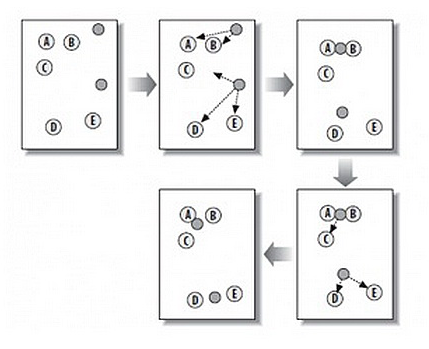
\includegraphics{figure2_1}
\caption{K-MEANS算法原理示意图}
\label{fig:2_1}
\end{figure}
\par DJ-Cluster是Zhou C在2007年提出的一种基于DBSCAN的聚类算法\upcite{zhou2007discovering}。DJ-Cluster算法的基本思想是计算每个点的密度,若密度值小于某给定值$MinPts$,且其所有邻居密度都小于给定值,则该点为异常点;否则,若该点所有邻居都不属于一个存在类别,则新建一个类别;否则与邻居中存在的类别合并。算法原理示意见图\ref{fig:2_2}。密度的定义见公式\ref{equ:chap2:dj-cluster}。 点$p$的密度是$N(p)$中元素的个数,$N(p)$是点$p$所有邻居组成的集合。$dist(p,q)$指$p$和$q$之间的欧氏距离。该算法聚类效果依赖$Eps$和$MinPts$两个常量的设置,且对这两个参数比较敏感。
\begin{equation}
\label{equ:chap2:dj-cluster}
N(p)=\{q \in S|dist(p,q) \leq Eps\}
\end{equation}
\begin{figure}[htp]
\centering
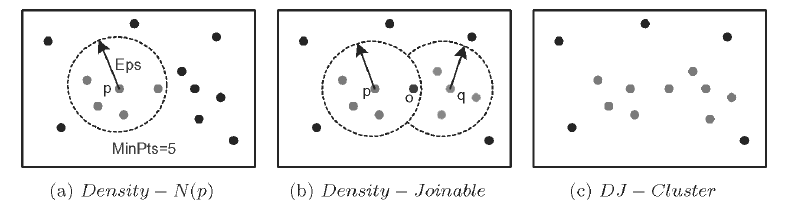
\includegraphics[width=6in]{figure2_2}
\caption{DJ-cluster聚类算法原理示意\upcite{zhou2007discovering}}
\label{fig:2_2}
\end{figure}
\par Rodriguez A等人2014年在Science上发表了一种新的基于密度的聚类算法\upcite{rodriguez2014clustering}。该算法不需要类别个数的先验知识,对参数也不敏感。该算法的基本思想是:计算每个点的密度(定义见公式\ref{equ:chap2:dj-cluster});计算每个点的距离,定义为该点与密度大于该点的所有点中距离最近的点之间的距离,若该点密度最大,则距离为所有点中与该点距离最远的点之间的距离;按距离对所有点排序,取前面若干个点作为聚类中心(若相邻两个点值差别非常大则以较大点作为聚类中心最后一个点);每个点的类别与密度大于自己且距离最近的点的类别一致。算法原理示意见图\ref{fig:2_3}和图\ref{fig:2_4}。
\begin{figure}[htp]
\centering
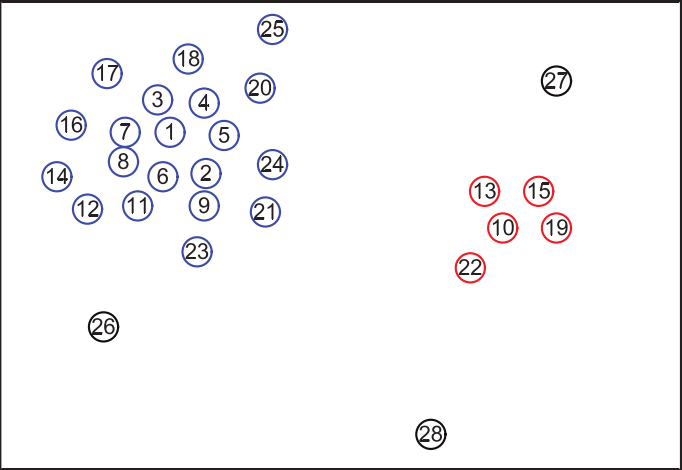
\includegraphics[width=4in]{figure2_3}
\caption{按密度排序\upcite{rodriguez2014clustering}}
\label{fig:2_3}
\end{figure}
\begin{figure}[htp]
\centering
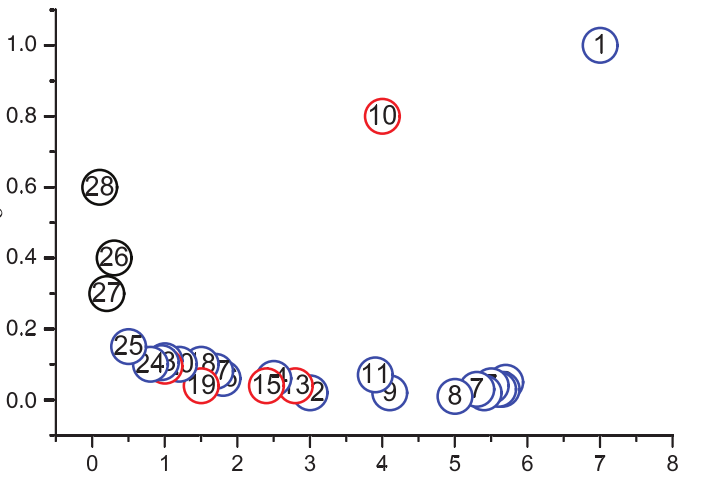
\includegraphics[width=4in]{figure2_4}
\caption{按距离排序,1、10为聚类中心\upcite{rodriguez2014clustering}}
\label{fig:2_4}
\end{figure}
\par 总的来说,上述三种聚类算法通过精心调整参数都能取得非常好的聚类效果。不同的算法拥有不同的优缺点,在第四章我们将通过实验来展示各种算法在不同参数下的聚类结果。
\section{时间序列相似度度量方法及序列熵值}
\label{sec:section2-2}
空间距离能够直观反映用户在物理世界的距离。根据社会心理学的研究成果,文献\upcite{festinger1977leon} 在一个大型住宅区研究了接近性效应(接近性效应指两个人住的越近越可能是朋友),结果表明人们居住得越近,不管这种近是物理距离还是功能性距离,人们越容易称为朋友。文献\upcite{zajonc1968attitudinal}用实验证实了单纯接触效应,即熟悉性能够促进好感,实验结果表明接触频率越高喜欢程度越大。而空间距离非常接近的用户在现实生活中会有更多的面对面的交互,从而增强两个人之间的关系强度。通过日常生活体验我们也很容易发现,如果两个人在晚上等休息时间经常一起出去,则其关系可能更亲密,因而他们之间的轨迹越可能相似。因此,我们可以使用熵值来度量用户每天活动的多样性,若某天活动越多样,则该天轨迹的相似度对总体轨迹的相似度贡献越大,进而对用户之间的关系强度贡献越大。
\par 用户的轨迹序列由带有时间戳的位置数据构成,位置数据可能是GPS 也可能是基站号。因此我们可以将轨迹序列看作时间序列,从而使用一些时间序列相似度度量模型来度量轨迹的相似度,下面依次描述编辑距离和DTW这两种相似度度量方法以及序列熵值的计算方法。
\subsection{编辑距离}
编辑距离是Levenshtein于1965年提出的一种度量两个字符串之间距离大小的方法\upcite{levenshtein1966binary},又称为Levenshtein距离。其定义为一个字符串通过插入,删除,改变这三种操作转变为另一个字符串所需要的最少的操作的步数。插入操作是指在某个位置添加一个字符;删除操作是指删除某位置的字符;改变操作是指把某个字符变成另外一个字符。
\par 若直接计算编辑距离会发现其时间复杂度为指数级别从而使得实际不可计算。通过深入分析发现该问题存在重叠子问题和最优子结构,因此可以用动态规划的思想把算法复杂度降低到多项式级别。其递推公式见公式\ref{equ:chap2:edit_distance},其中$s1$,$s2$ 表示两个字符串,$M[i,j]$表示字符串$s1[0:i]$ 和字符串$s2[0:j]$ 之间的编辑距离。$E[i,j]$指$s1[i]$ 和$s2[j]$ 之间的距离,若两个字符相同,则距离为0,否则距离为1。
\begin{equation}
\label{equ:chap2:edit_distance}
M[i,j] = min(M[i–1,j],M[i,j–1],M[i–1,j–1] + E[i,j])
\end{equation}
\par 编辑距离的计算对象是字符串,因此,经过一些学者的研究,将其扩展到实数域\upcite{chen2005robust},称为EDR(Edit Distance on Real sequence),并对每个操作附加权重\upcite{chen2004marriage},称为ERP(Edit distance with Real Penalty)。在实数域中,若两个实数非常接近,则认为这两个数相等,否则认为不相等。ERP对两个相等的数用这两个数的差作为实数惩罚值,否则用其中一个数与一个常量的差做为实数惩罚值。其计算过程与原始编辑距离计算过程类似。
\subsection{Dynamic Time Warping}
DTW(Dynamic Time Warping)是Itakura于1987年提出的距离度量方法\upcite{itakura1987distance},主要用于识别两个读音是否表示同一个单词,Berndt\upcite{berndt1994using} 使用DTW方法来度量时间序列的相似度,从而发现时间序列中的模式。
\par 假设有两个时间序列,序列$Q$长度为$n$ (见公式\ref{equ:chap2:dtw_01}),序列$C$ 长度为$m$ (见公式\ref{equ:chap2:dtw_02})。为了计算两个序列之间的DTW 距离,需要构造一个$n \ast m$矩阵$d$,其中$d[i,j]$ 表示序列$Q$ 第$i$个元素$q_{i}$ 和序列$C$第$j$ 个元素$c_{j}$之间的距离,通常使用欧氏距离作为两个元素之间的距离度量。构造$n \ast m$ 矩阵$\gamma$。为了寻找这两个序列之间的最佳匹配,需要寻找一条路径使得累积距离$\gamma[i,j]$最小化,可以通过使用动态规划的方法来找到这条路径,$\gamma[n,m]$ 为最终的DTW距离,其递推公式见公式\ref{equ:chap2:dtw_03}。$d[i,j]$指$q_{i}$ 和$c_{j}$ 之间的欧式距离。$\gamma[i,j]$是指当前的累积距离,路径及矩阵可视化见图\ref{fig:2_5}。其中:A)两个异相的相似序列Q 和C;B)为了匹配这两个序列,构造了一个变形矩阵,并搜索最佳的变形路径即红色所示路径,且将搜索局限到一个窗口中;C) 匹配结果
\begin{equation}
\label{equ:chap2:dtw_01}
Q=q_{1},q_{2},…,q_{i},…,q_{n}
\end{equation}
\begin{equation}
\label{equ:chap2:dtw_02}
C=c_{1},c_{2},…,c_{j},…,c_{m}
\end{equation}
\begin{equation}
\label{equ:chap2:dtw_03}
\gamma[i,j]=d[i,j]+min\{\gamma[i-1,j-1],\gamma[i-1,j],\gamma[i,j-1]\}
\end{equation}
\begin{figure}[htp]
\centering
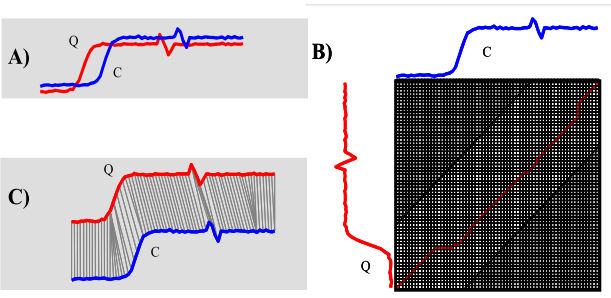
\includegraphics[width=4in]{figure2_5}
\caption{引自文献\cite{ratanamahatana2004everything}DTW原理示意图。}
\label{fig:2_5}
\end{figure}
\par 通过深入分析DTW算法可知,序列的长度越长,则距离可能越大。因此,采用文献\cite{ratanamahatana2004everything} 中的三种归一化方法对DTW的计算结果进行进一步的处理和优化,即DTW结果除以最优变形路径的长度、DTW结果除以两个序列中较短序列的长度以及DTW结果除以两个序列中较长序列的长度等三种方法对DTW计算结果进行归一化,以便获得最优结果。
\subsection{序列熵值}
通过对用户每天产生的轨迹序列的分析,可以将其看作一个由一系列随机变量$X_{n}$构成的随机过程序列$X=\{X_{1},X_{2},…,X_{n}\}$,$X_{n}$表示用户在时刻$n$ 所在的物理位置。熵通常用来度量一个系统的无序程度,熵越大表示该系统越混乱。若用户每天活动单一,则熵值会很小,若活动多样,则熵值会越大。因此,可以用熵值来度量用户每天活动的多样性程度,香农熵的定义见公式如公式\ref{equ:chap2:se_01},其中$P(x_{i})$是$x_{i}=X_{i}$的概率。
\begin{equation}
\label{equ:chap2:se_01}
H=-\sum_{i}p(x_{i})log_{2}p(x_{i})
\end{equation}
\par 对于一个长度为n的随机变量序列,需要考虑该序列的熵值如何随n增长,这个增长率称为熵率,熵率定义见公式\ref{equ:chap2:se_02}。同时,熵率存在一个相关的量,定义见公式\ref{equ:chap2:se_03}。 对于平稳随机过程,这两种定义的极限均存在且相等\upcite{cover2012elements}。
\begin{equation}
\label{equ:chap2:se_02}
H(\aleph)=lim_{n \rightarrow \infty} \frac{1}{n}H(X_{1},X_{2}...,X_{n})
\end{equation}
\begin{equation}
\label{equ:chap2:se_03}
H^{'}(\aleph)=lim_{n \rightarrow \infty} H(X_{n}|X_{n-1},X_{n-2}...,X_{1})
\end{equation}
\par 由于条件熵值(公式\ref{equ:chap2:se_03})难以直接计算,因此通常使用估量值来计算熵率,常用的估量值主要包括LZ (Lempel-Ziv)估量值\upcite{kontoyiannis1998nonparametric}以及实时LZ估量值\upcite{mcinerney2013breaking} 等。LZ估量值的定义见公式\ref{equ:chap2:se_04},其中$\gamma_i$定义为从位置$i$ 开始,不在序列$(X_{1},X_{2},…,X_{i-1})$中出现的最短的子序列的长度。实时LZ 估量值的定义见公式\ref{equ:chap2:se_05} 和公式\ref{equ:chap2:se_06},其中$\delta_i$定义为以位置$i$结尾,不在序列$(X_{1},X_{2},…,X_{i-\delta_i})$ 中出现的最短的子序列的长度。这两种度量实际上是等价的,在本文中我们使用实时LZ 估量值,该估量值只利用当前已知的信息。
\begin{equation}
\label{equ:chap2:se_04}
\hat{H}_{N}=(\frac{1}{N-1}\sum_{i=2}^{N}\frac{\gamma_i}{log_{2}(i)})^{-1}
\end{equation}
\begin{equation}
\label{equ:chap2:se_05}
\tilde{H}_{i}=\frac{log_{2}(i)}{\delta_i}
\end{equation}
\begin{equation}
\label{equ:chap2:se_06}
\hat{H}_{N}=\frac{N}{\sum_{i=2}^{n}\tilde{H}_{i}^{-1}}
\end{equation}
\par 计算轨迹序列的熵值的目的是为了对DTW计算结果进行加权,因为用户每天的轨迹序列的相似度对其总体相似度的贡献是不一样的,如果某一天用户的轨迹序列的熵值越大,则这一天对总的相似度贡献越大,因此,使用用户当天轨迹序列熵值对用户与朋友之间每天的轨迹相似度进行加权,能够更真实地反应用户之间的关系强度(如何使用轨迹序列熵值对DTW 的计算结果进行加权详见第五章第三小节)。
\par 编辑距离和DTW都是非常常用的两种时间序列相似度度量方法,在第六章我们将通过实验展示这两种方法以及用序列熵值加权后的两种方法用来度量用户关系强度的效果
\section{自然语言处理模型}
\label{sec:section2-3}
在日常生活当中,用户之间尤其是好友之间其行为模式之间具有一定的相似性,如经常去某些地方、经常在某些时间段(晚上)去一些地方(餐馆、酒吧)等等。基于位置的用户行为模式一方面能够反映用户在物理层次的相遇,另一方面能够在一定程度上体现用户的相似性,前文已经从社会心理学的角度阐述了相遇次数与用户关系强度的关系,Singelis\upcite{singelis1994measurement}认为人们倾向于喜欢在态度、兴趣、价值观、背景和人格上和其相似的人,因此,在日常生活当中行为相似的人之间更可能成为朋友,而根据社会心理学的研究成果,用户的相似性对用户的关系强度也有一定的影响,为此,在通过基于用户轨迹度量用户之间关系强度的基础上,进一步通过基于位置的用户日常行为来对度量用户之间的关系强度。
\par 通过将位置序列和自然语言中的句子进行类比,能够发现,自然语言处理中的这些方法可以很自然的用来处理位置轨迹数据。位置序列是用户轨迹语义层次的一种表示,例如一个学生一天的位置轨迹可以表示为宿舍、实验室、食堂、宿舍,实验室、食堂、宿舍。通过深入分析,认为自然语言中的每个句子受两方面的约束,即主观约束和客观约束。客观约束指句子的构造受到对应语言语法的约束;主观约束指在句子的构造过程中,部分词的使用和构造者的个人喜好相关。再来分析一下位置序列,位置序列的构成也受主观和客观这两方面的约束,客观约束指用户自身的社会角色限制了用户每天可能的位置序列;主观约束指用户在客观约束下,对于一些位置具有选择性,如用户可以自己决定去什么地方吃饭等。
\par 文献\cite{farrahi2008did}最先使用LDA主题模型发现用户的行为模式,在使用LDA 模型发现用户基于位置的行为模式基础上,本课题进一步使用LDA 主题模型来度量用户之间的关系强度,其核心思想如下:把每个用户每天参观过的位置(物理位置或语义位置)序列视为一个句子,每个用户所有天的位置序列视为一篇文档,对所有用户所有天的位置序列使用LDA主题模型训练得到若干个主题。在计算两个用户之间的关系强度时,将这两个用户同一天的数据按固定长度的时间片划分,对于每个时间片内用户参观过的位置,用训练好的LDA主题模型推断这些位置对应的主题分布,以同一时间片内,两个用户分别参观过的位置对应的主题分布的余弦相似度,作为这两个用户之间的关系强度(详细的计算过程见第五章第三节)。
\par word2vec模型主要通过考虑当前词语的上下文环境来得到当前词语对应的实数值向量表示。而对应向量的相似度从一定程度上反映了两个词语义的相似度。因此在计算出每个语义位置对应的实数值向量后,希望对应向量的相似度能够从一定程度上反应两个语义位置功能的相似性。
\subsection{Latent Dirichlet Allocation}
LDA(Latent Dirichlet Allocation)\upcite{blei2003latent}是Blei等人2003 年提出的一个针对离散数据集合的产生式概率模型。LDA是一个三层的层级贝叶斯模型(其结构如图\ref{fig:2_6} 所示), LDA模型作为一个文本模型,每个文档由多个主题的概率分布来表示,每个主题由多个单词的分布来表示,图\ref{fig:2_6}中每个方框表示执行,外框表示文档,内框表示文档内主题和单词的重复选取。假设有$K$个主题,$W$个不同单词,一个给定词$\omega_{t}$的概率见公式\ref{equ:chap2:lda_01},其中$z_{t}$表示产生第$t$个词的主题对应的隐变量。
\begin{equation}
\label{equ:chap2:lda_01}
p(\omega_{t})=\sum_{k=1}^{K}p(\omega_t|z_{t}=k)p(z_{t}=k)
\end{equation}
\begin{figure}[htp]
\centering
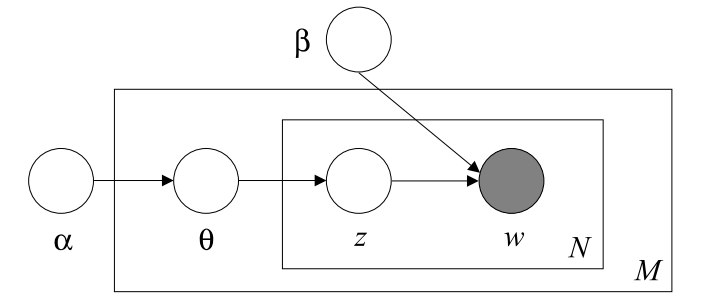
\includegraphics[width=4in]{figure2_6}
\caption{LDA的图模型表示\upcite{blei2003latent}}
\label{fig:2_6}
\end{figure}
\par LDA推断的目的是计算每个主题的词分布$P(w|z=k)=\varphi_{w}^{(k)}$和每个文档的主题分布$P(z=k)=\theta_{k}^{(d)}$。在LDA 中,$P(\theta)$服从$Dirichlet(\alpha)$分布,$p(\varphi)$服从$Dirichlet(\beta)$分布,其中$\alpha$和$\beta$是超参数。LDA模型的估计问题等同于求公式\ref{equ:chap2:lda_02}的最优值问题,但其计算非常复杂,故使用MCMC(Markov Chain Monte Carlo)方法求得近似解,其采样公式见公式\ref{equ:chap2:lda_03},其中$n_{k}^{(\omega)}$和$n_{k}^{(d)}$是单词$\omega$和文档$d$分配给主题$k$的次数。
\begin{equation}
\label{equ:chap2:lda_02}
p(\omega|\varphi,\alpha)=\int p(\omega|\varphi,\theta)p(\theta|\alpha)d\theta
\end{equation}
\begin{equation}
\label{equ:chap2:lda_03}
\varphi_{k}^{(\omega)}=\frac{n_{k}^{(\omega)}+\beta}{n_{k}^{(.)}+W\beta},\theta_{k}^{(d)}=\frac{n_{k}^{(d)} + \alpha}{n_{.}^{(k)}+K\alpha}
\end{equation}
\subsection{word2vec}
随着深度学习的提出,概率语言模型也有了新的发展。当前已经有很多深度学习框架的自然语言处理模型,word2vec\upcite{mikolovword2vec}是应用最广泛的一种。word2vec共有四种模型,主要描述第一种使用Hierarchical Softmax 的CBOW(Continuous Bag-of-Words Model)模型。该模型主要思想是依据已知当前词$w_{t}$的上下文$w_{t-2}$,$w_{t-1}$,$w_{t+1}$,$w_{t+2}$的前提下预测当前词$w_{t}$。该模型包括输入层,投影层和输出层。其网络结构\upcite{peghotyw2v}如图\ref{fig:2_7} 所示。
\begin{figure}[htp]
\centering
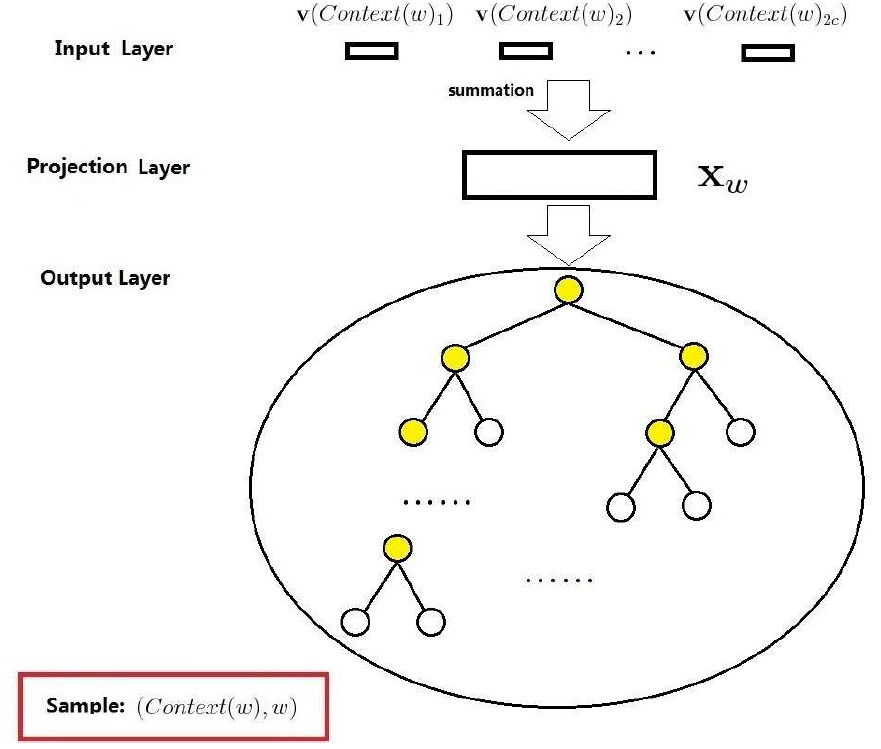
\includegraphics[width=4in]{figure2_7}
\caption{word2vec神经网络结构图\upcite{peghotyw2v}}
\label{fig:2_7}
\end{figure}
\par 输入层:由$Context(w)$中$2c$个词的词向量组成,每个词向量长度为$m$;投影层:对输入层的$2c$个词向量按分量累加求和;输出层:输出层对应一棵二叉树,它以语料中出现过的词作为叶子节点,且以其出现次数为权值构造出来的Huffman树。
\par 对词典$D$中的任意一个词$w$,Huffman树中必存在一条从根节点到词$w$(该词对应一个叶子节点)对应节点的路径(且这条路径是唯一的)。路径上存在大量分支,而每个分支可以看做一次二次分类,每一次分类产生一个概率,将这些概率全部乘起来,就是所需的$p(w|Context(w))$。条件概率的一般公式可以写成公式\ref{equ:chap2:w2v_01} 和\ref{equ:chap2:w2v_02}。
\begin{equation}
\label{equ:chap2:w2v_01}
p(w|Context(w)=\Pi_{j=2}^{1^{w}}p(d_{j}^{w}|x_{w},\theta_{j-1}^{w})
\end{equation}
\begin{equation}
\label{equ:chap2:w2v_02}
p(d_{j}^{w}|x_{w},\theta_{j-1}^{w})=[\sigma(x_{w}^{T}\theta_{j-1}^{w})]^{1-d_{j}^{w}}\ast[1-\sigma(x_{w}^{T}\theta_
{j-1}^{w})]^{d_{j}^{w}}
\end{equation}
\par $1^{w}$表示从根节点到节点$w$路径上所有节点的个数,$d_{j}^{w}$表示路径上第$j$个词,$x_{w}$表示词$w$对应的词向量,$\theta_{j-1}^{w}$表示路径上第$j$个非叶节点对应的向量。$\sigma$表示SIGMOID函数。
\par 故该神经网络的目标函数见公式\ref{equ:chap2:w2v_03}。
\begin{equation}
\label{equ:chap2:w2v_03}
L=\sum_{w\in C}\sum_{j=2}^{1^{w}}\{(1-d_{j}^{w})log[\sigma(x_{w}^{T}\theta_{j-1}^{w})]+d_{j}^{w}log[1-\sigma(x_{w}^{T}\theta_{j-1}^{w})]\}
\end{equation}
\par 使用随机梯度上升法求得该目标函数局部最大值,即可得到每个词对应词向量。
\par LDA和word2vec在自然语言处理相关的应用中都得到了非常好的结果,因此使用这两个算法度量用户之间的关系强度,在第五章详细描述如何使用这两种方法度量用户之间的关系强度,在第六章将通过实验展示这两个模型在不同的参数下对实验结果的影响。
\section{小结}
\label{sec:section2-4}
本章对与课题密切相关的三方面技术进行的详细的描述、分析和研究。2.1节描述了GPS预处理中遇到的两个主要问题降噪和聚类。2.2节描述了度量时间序列相似度的两种常见方法以及序列熵值的计算方法,前两种方法用于计算轨迹序列的相似度,并以此相似度作为用户之间的关系强度,在此基础上用序列熵值对对轨迹序列的相似度加权。2.3节描述了LDA和word2vec两种常见的自然语言处理模型,这两种模型能够从不同的角度反映用户基于轨迹的行为模式。
\chapter{用户关系强度层级投票模型框架}
\label{chap:chapter07}
上一章描述了与本课题密切相关的三方面技术,这一章我们主要描述本课题的整体模型框架。
\section{模型框架描述}
\label{sec:section7-1}
本课题主要目标是利用用户的轨迹数据度量用户之间的关系强度。轨迹数据分为GPS数据和基站数据两种,本课题尝试提出一个通用的关系强度计算模型框架,希望能够使用同一个框架处理GPS数据和基站数据,见图\ref{fig:7_1}。但是GPS数据和基站数据在数据特性上有非常大的区别,GPS是连续实数值,且有实际物理意义,而基站数据只是一个标号,数值本身没有实际物理意义,需要分别对GPS数据和基站数据进行处理,GPS数据相较于基站数据而言,表示的物理位置更加精确,故需要一些额外的方法获取GPS 数据的高层信息,比如物理位置、语义标签等。GPS采样本身仍然存在误差,需要使用一定的方法来降低采样数据的误差。GPS数据相较基站数据而言,需要更多的处理,一方面降低自身的误差,另一方面获取更高层信息。第四章将主要描述如何处理GPS数据以及如何获取更高层信息,对应该模型框架左边的SASLL系统。第五章将主要描述如何使用轨迹数据度量用户之间的关系强度,本课题主要从原始轨迹数据、语义位置、语义标签三个层次来度量用户之间的关系强度,每一层输入数据的准备过程将在第四章第二节详细描述,GPS 数据的准备过程基于第四章提出的相关的处理技术。同样基站数据作为模型三层输入数据的准备过程也将在第四章第二节详细描述,基站数据的处理非常简单,不需要额外的技术,该模型右边相关模块简要说明了基站数据对应的三层模型输入数据的处理过程。
\begin{figure}[htp]
\centering
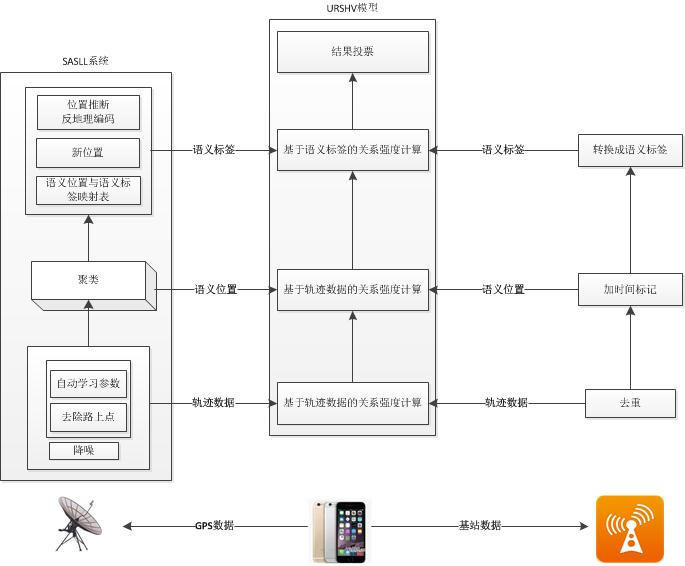
\includegraphics[width=4in]{figure7_1}
\caption{用户关系强度层级投票模型框架图}
\label{fig:7_1}
\end{figure}
\subsection{SASLL系统概述}
SASLL是一个语义标签标注系统,使用传感器数据采集软件记录手机传感器数据,GPS数据模块通过访问本地传感器数据存储文件,读入GPS数据相关的数据文件,并对文件数据进行JSON 解析,得到原始GPS数据记录,每条记录格式为由经度、维度、时间戳组成的三元组(Lat,Lng,timestamp)。预处理模块在本系统第一次执行时自动学习剔除路上点需要的参数,并使用基于密度的方法剔除路上的点,之后对于每天的数据使用分段卡尔曼滤波对原始GPS数据进行滤波,以降低数据的噪声。聚类模块对每天采集的数据使用文献\cite{rodriguez2014clustering}提出的聚类算法对预处理后的数据进行聚类,该算法在第一次运行时需要根据数据的特性设置阈值参数,然后得到每天参观过的位置,并与已标记表进行对比,计算得到新的位置。位置提示模块对新位置使用基于规则的推断方法推断新位置是否是家或办公室,如果都不是则调用地图接口计算反地理编码的方法计算其可能的语义标签,如果无对应反地理编码结果,则由用户手动输入新位置的语义标签。最后由交互模块和用户交互,展示位置提示模块计算的提示以及记录用户的标注。
\subsection{用户关系强度计算模型概述}
要真实全面反映人们之间的关系强度,需要从不同角度和不同层次对人们之间的关系强度进行度量,为此,我们提出了一个层次化的、对用户关系强度进行度量、并对度量结果进行投票的模型URSHV,其框架结构如图\ref{fig:7_1}中间部分所示。URSHV模型是一个三层的、能够对通过GPS 和基站这两种方式采集的数据进行处理的度量模型,从轨迹、语义位置以及语义标签三个层次对人们之间的关系强度进行度量,并使用集成学习的思想对三个层次度量结果进行投票,最终以投票结果作为人们之间的关系强度。第一层度量主要针对用户的轨迹序列数据,考虑真实生活中,用户和用户之间的共同出现情况以及用户和用户之间错时出现情况(用户轨迹序列相似,但相同地方出现时间具有相同的滞后或超前),根据不同用户轨迹序列的相似度来度量用户之间的关系强度;第二层度量主要针对用户的语义位置序列数据,考虑用户个人的基于位置的行为模式如经常在什么时间出现在哪些位置等,根据不同用户行为模式的相似度来度量用户之间的关系强度;第三层度量主要针对用户的语义标签序列数据,物理上不同的位置可能拥有相同的语义标签,“办公室”、“家”等语义概念在每个用户轨迹中都可能出现,而这些语义概念在原始数据中会表现为不同的基站号和区域号或不同的GPS经纬度,因此用户的语义位置数据更能体现用户群体的日常习惯,因此本层考虑的行为模式更倾向于群体的行为模式,从而根据不同用户在群体中表现出的行为模式来度量用户之间的关系强度。
\section{模型完整流程描述}
\label{sec:section7-2}
首先使用采集应用记录手机传感器数据,包括GPS数据和基站数据。
其次,对采集的GPS数据和基站数据分别进行处理。处理GPS数据:对GPS数据使用分段卡尔曼滤波算法进行降噪处理,对每天的GPS 数据进行划分,等时间均分为若干份,对每份数据计算其GPS经纬度均值作为这段时间的GPS数据,通过这样处理以后,可以把每天的GPS序列降到一个比较小的维度,其长度等于按时间均分的份数。处理基站数据:对每天的基站数据进行划分,等时间均分为若干份,对每份数据进行集合操作,使得该份数据内,基站不重复,把每一份数据重新拼成一个基站序列。计算两个用户的关系强度时,对每个用户每天的数据按前文所述进行处理,处理完后,对两个用户每天处理完成的GPS序列或者基站序列计算其DTW 距离,计算处理完成的GPS序列或基站序列对应的序列熵值,用该熵值对前面计算的DTW 距离进行加权,对每天加权后的距离计算加权平\\par 均值,以此作为两个用户关系强度的度量。
再次,对降噪后的GPS数据剔除路上的点,使用聚类算法得到对应的语义位置,将GPS序列转换成对应的语义位置序列,对每个语义位置添加时间标记;对基站数据添加时间标记。训练对应的LDA主题模型。计算两个用户的关系强度时,将前文得到的语义位置序列按等时间间隔划分成若干份,基站数据采用同样的处理,对每一份数据推断其对应的LDA主题分布,得到一个若干维的实数值向量。计算两个用户每天同一时间段的两份数据对应的主题分布的余弦相似度,计算全天的平均相似度,以及全部数据的平均相似度,以此作为两个用户关系强度的度量。
\par 再次,对聚类后得到的语义位置标记其对应的语义标签,将语义位置序列转换成对应的语义标签序列,对每个语义标签添加时间标记;将每个基站转换成对应的语义标签,对每个语义标签添加时间标记。训练对应的LDA主题模型。计算用户关系强度的方法与前文基于语义位置计算关系强度的方法相同。
\par 最后,在前面三层计算结果的基础上,对三层关系强度的计算结果进行投票,将投票结果作为最终的关系强度。
\chapter{GPS数据处理及语义标签标注技术}
\label{chap:chapter03}
上一章主要描述了本课题的整体模型框架。本章描述该整体模型框架的第一部分GPS数据处理及语义标签标注技术,包括SASLL 系统框架、如何计算GPS 数据对应的语义位置以及如何对语义位置标语义标签。
\section{SASLL标注技术}
\label{sec:section3-1}
SASLL(A System Annotating Semantic Label of Location)标注技术原理如图\ref{fig:3_1},GPS数据模块访问本地传感器数据存储文件,对文件数据进行解析,得到GPS原始数据,其格式为由经度、维度、时间戳组成的三元组(Lat,Lng,timestamp)。预处理模块在本系统第一次执行时自动学习剔除路上点需要的参数,并使用基于密度的方法剔除异常点。聚类模块对当天采集的数据使用\upcite{rodriguez2014clustering}提出的算法对预处理后的数据进行聚类,得到当天参观过的位置,并与匹配表进行对比,计算得到新的位置。位置提示模块对新位置使用基于规则的推断方法和调用地图接口计算反地理编码的方法计算其可能的语义标签。最后由交互模块和用户交互,展示位置提示模块计算的提示以及记录用户的标注。
\begin{figure}[htp]
\centering
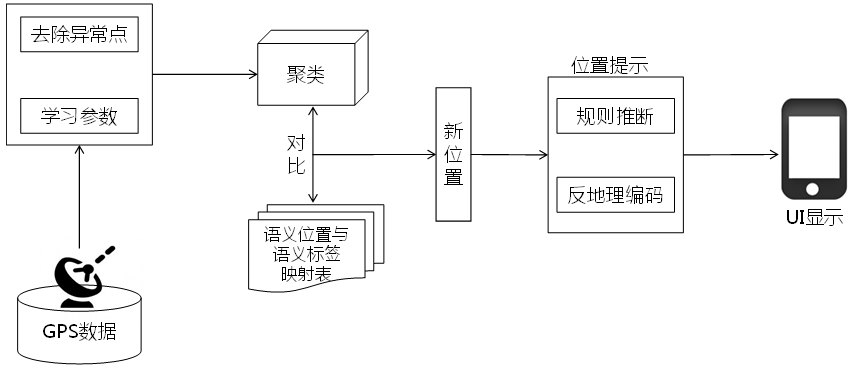
\includegraphics[width=6in]{figure3_1}
\caption{SASLL系统框架图}
\label{fig:3_1}
\end{figure}
\section{计算对应语义位置}
\label{sec:section3-2}
本节主要描述如何通过GPS发现语义位置,包括如何降低数据噪声、如何剔除异常点以及如何通过聚类得到语义位置。
\subsection{降低数据噪声}
根据自己的日常活动发现,用户会经常停留在某一固定位置很长时间,在这段时间内,其实用户本身位置是不变的,但是GPS采样值会包含一些随机误差,从而使得虽然实际上用户一直呆在同一个位置,采样得到的经纬度会在实际经纬度上下震荡。因此需要对GPS数据进行滤波使得采样值经过处理后更加接近实际值。第二章描述了常用的三种降噪方法,即均值滤波、中值滤波和卡尔曼滤波。算法原理不再赘述,这一小节主要通过实验来观察各种滤波算法的效果以及在实验的基础上提出分层卡尔曼滤波的方法。
\par 首先使用自己日常采集的某几天的数据来观察均值滤波的降噪效果,数据采集软件使用\upcite{rawassizadeh2013ubiqlog}。 如图\ref{fig:3_2_1}、\ref{fig:3_2_2}、\ref{fig:3_2_3}所示。
\begin{figure}[htb]
  \centering%
  \subfloat[原始数据]{%
    \label{fig:3_2_1_1}
    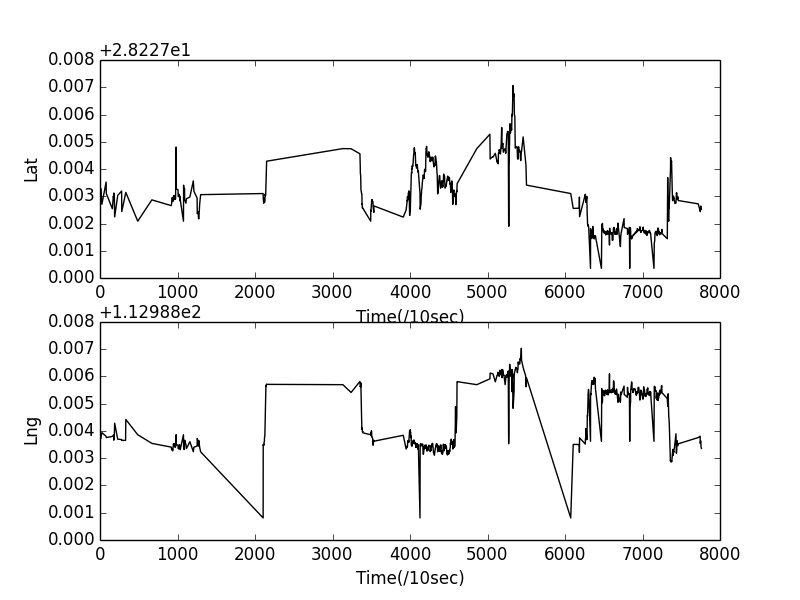
\includegraphics[height=4cm]{figure3_2_1_1}}\hspace{4em}%
  \subfloat[均值滤波]{%
    \label{fig:3_2_2_1}
    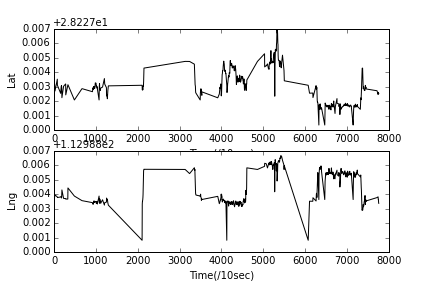
\includegraphics[height=4cm]{figure3_2_1_2}}
  \caption{均值滤波实验结果3-1}
  \label{fig:3_2_1}
\end{figure}
\begin{figure}[htb]
  \centering%
  \subfloat[原始数据]{%
    \label{fig:3_2_2_1}
    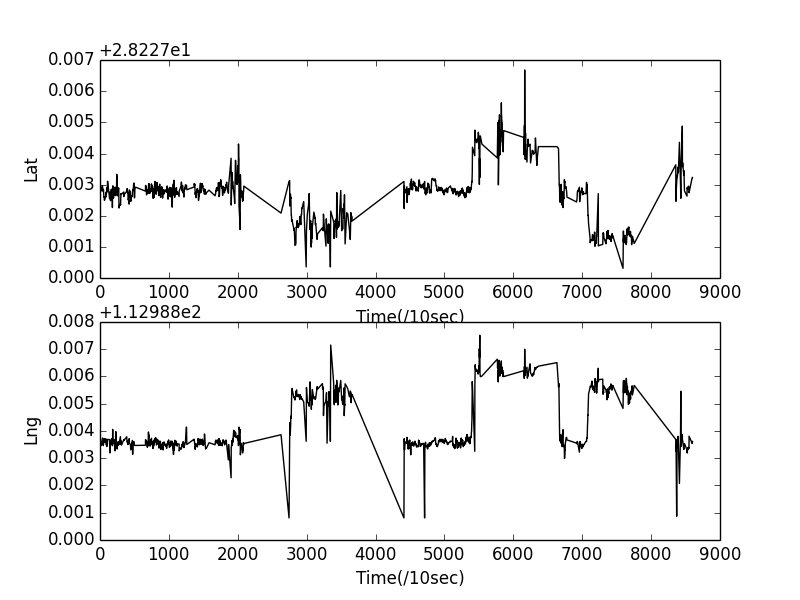
\includegraphics[height=4cm]{figure3_2_2_1}}\hspace{4em}%
  \subfloat[均值滤波]{%
    \label{fig:3_2_2_2}
    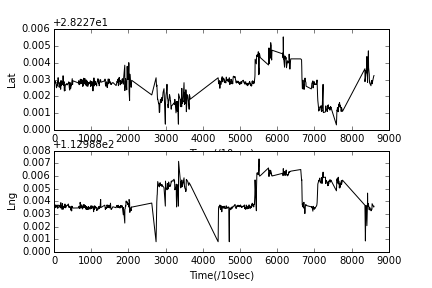
\includegraphics[height=4cm]{figure3_2_2_2}}
  \caption{均值滤波实验结果3-2}
  \label{fig:3_2_2}
\end{figure}
\begin{figure}[htb]
  \centering%
  \subfloat[原始数据]{%
    \label{fig:3_2_3_1}
    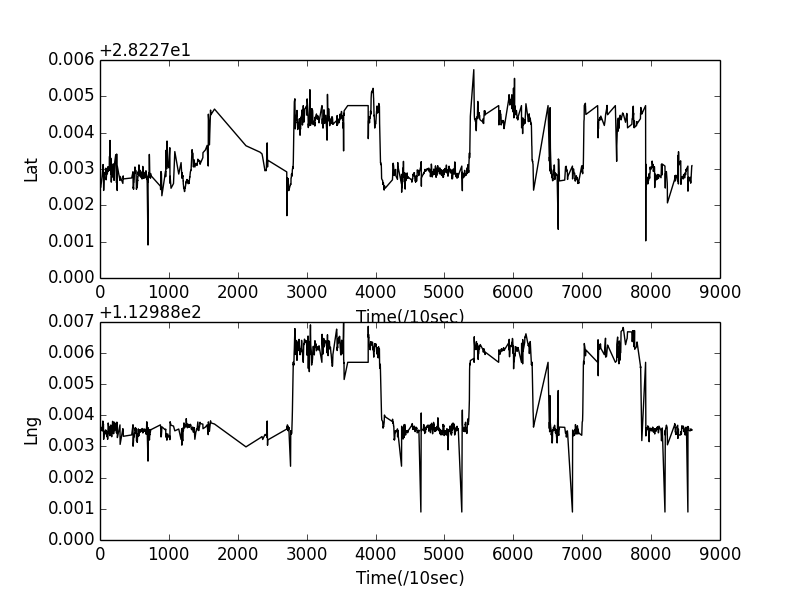
\includegraphics[height=4cm]{figure3_2_3_1}}\hspace{4em}%
  \subfloat[均值滤波]{%
    \label{fig:3_2_3_2}
    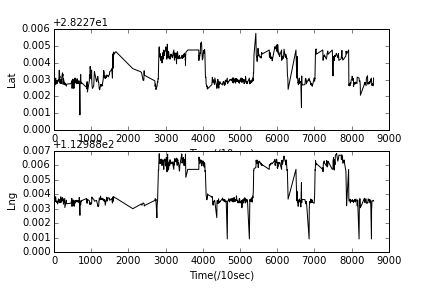
\includegraphics[height=4cm]{figure3_2_3_2}}
  \caption{均值滤波实验结果3-3}
  \label{fig:3_2_3}
\end{figure}
\par 仔细分析实验结果发现,虽然滤掉一少部分跳变点,但是对于非常明显的几个跳变点,均值滤波并没有滤掉。
\par 下文展示中值滤波的实验结果。实验结果见图\ref{fig:3_3_1}、\ref{fig:3_3_2}、\ref{fig:3_3_3}。
\begin{figure}[htb]
  \centering%
  \subfloat[原始数据]{%
    \label{fig:3_2_1_1}
    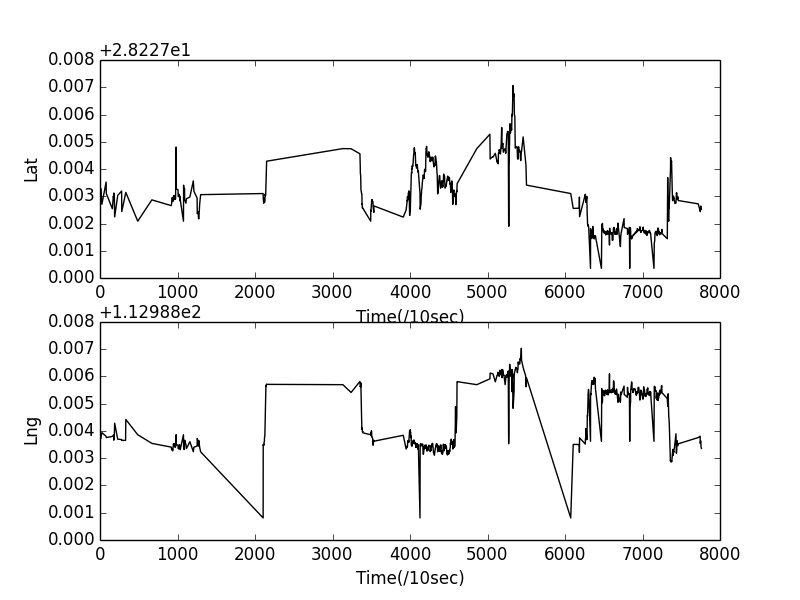
\includegraphics[height=4cm]{figure3_2_1_1}}\hspace{4em}%
  \subfloat[中值滤波]{%
    \label{fig:3_2_2_1}
    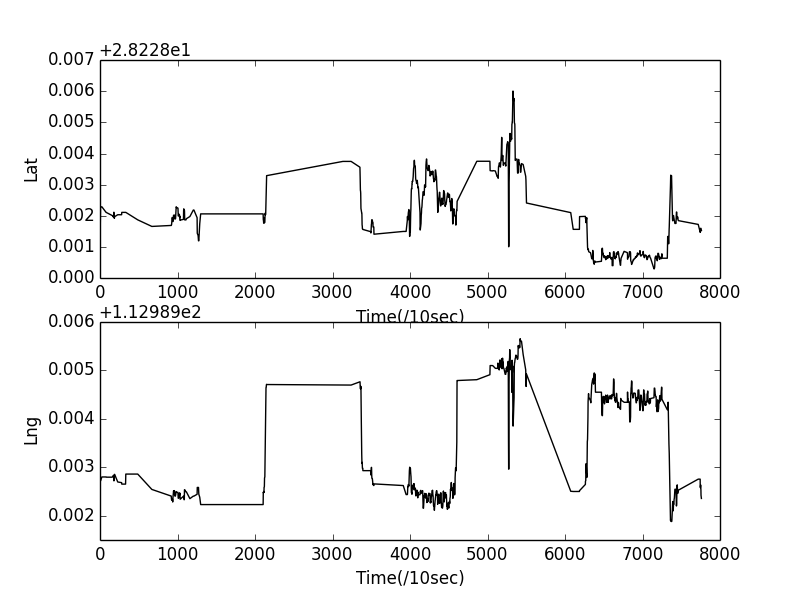
\includegraphics[height=4cm]{figure3_3_1_2}}
  \caption{中值滤波实验结果3-1}
  \label{fig:3_3_1}
\end{figure}
\begin{figure}[htb]
  \centering%
  \subfloat[原始数据]{%
    \label{fig:3_2_2_1}
    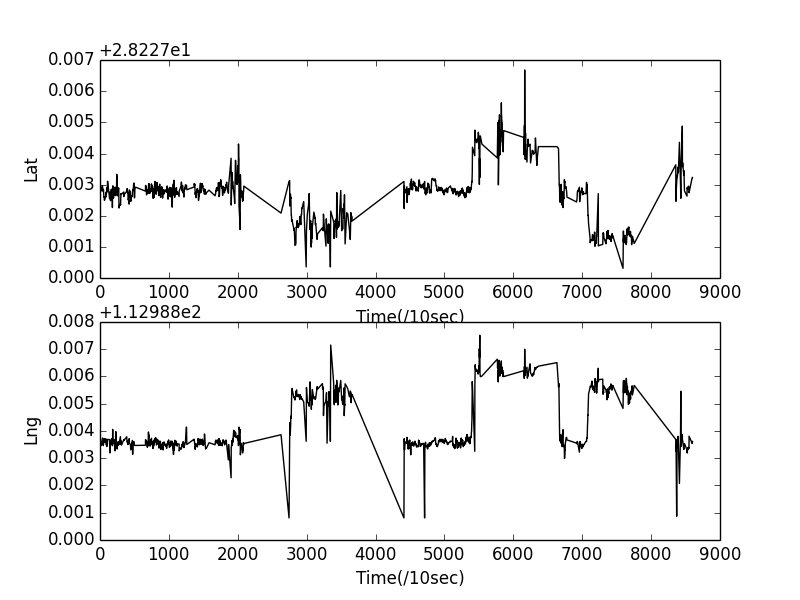
\includegraphics[height=4cm]{figure3_2_2_1}}\hspace{4em}%
  \subfloat[中值滤波]{%
    \label{fig:3_2_2_2}
    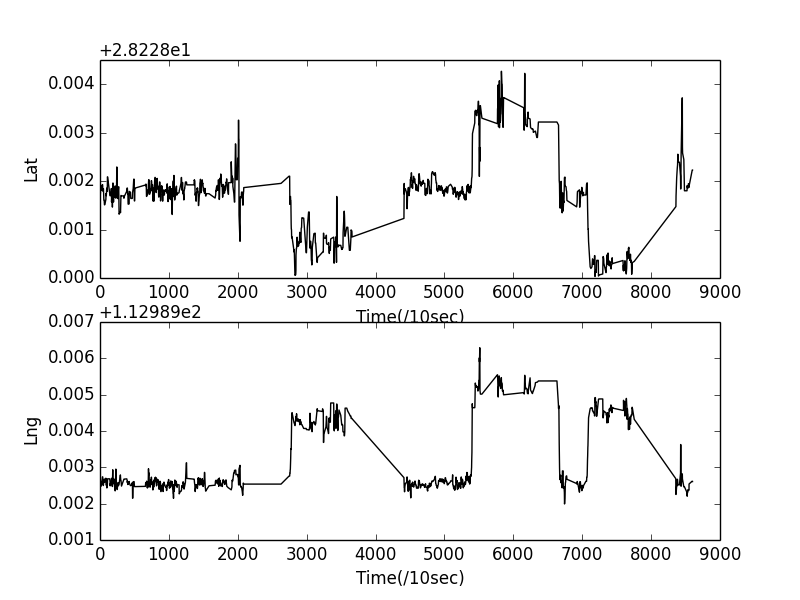
\includegraphics[height=4cm]{figure3_3_2_2}}
  \caption{中值滤波实验结果3-2}
  \label{fig:3_3_2}
\end{figure}
\begin{figure}[htb]
  \centering%
  \subfloat[原始数据]{%
    \label{fig:3_2_3_1}
    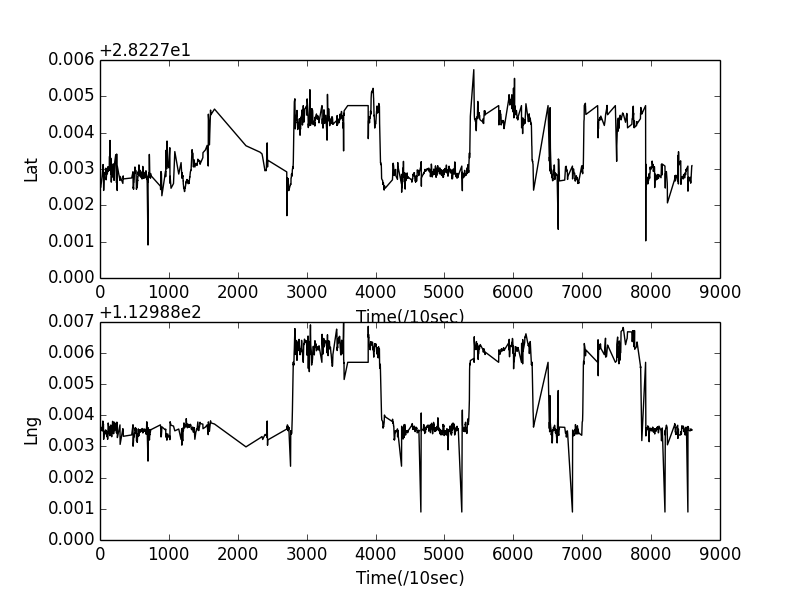
\includegraphics[height=4cm]{figure3_2_3_1}}\hspace{4em}%
  \subfloat[中值滤波]{%
    \label{fig:3_2_3_2}
    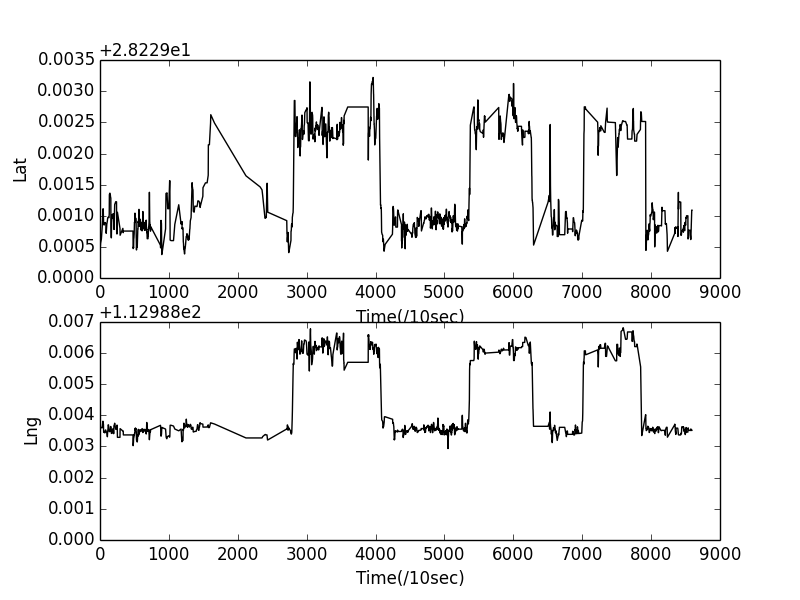
\includegraphics[height=4cm]{figure3_3_3_2}}
  \caption{中值滤波实验结果3-3}
  \label{fig:3_3_3}
\end{figure}
\par 仔细分析实验结果,中值滤波的结果明显好于均值滤波,滤除掉了大部分跳跃点。
\par 下文展示卡尔曼滤波的实验结果,实验结果见图\ref{fig:3_4_1}、\ref{fig:3_4_2}、\ref{fig:3_4_3}。
\begin{figure}[htb]
  \centering%
  \subfloat[原始数据]{%
    \label{fig:3_2_1_1}
    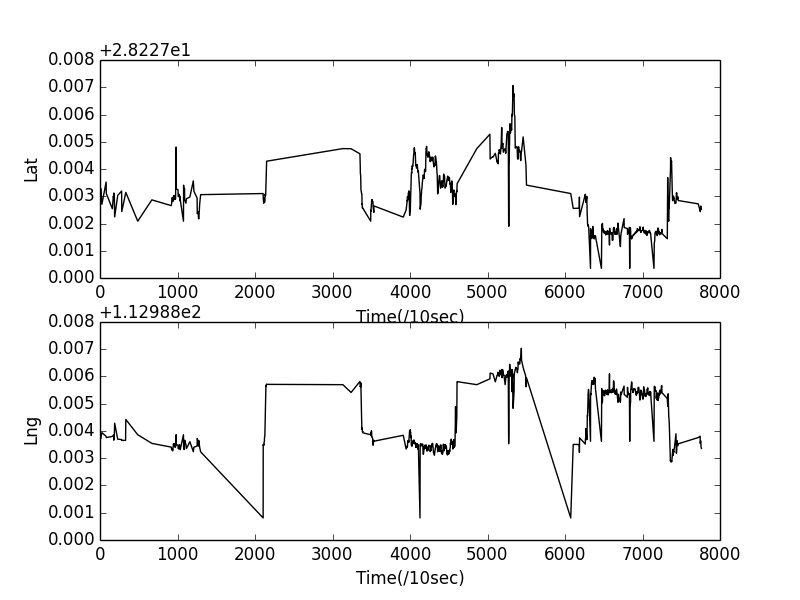
\includegraphics[height=4cm]{figure3_2_1_1}}\hspace{4em}%
  \subfloat[卡尔曼滤波]{%
    \label{fig:3_2_2_1}
    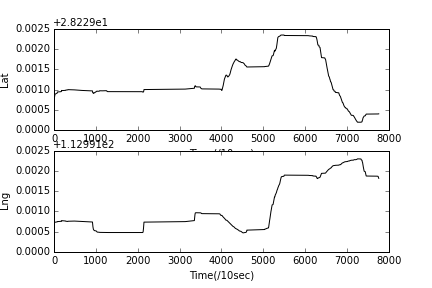
\includegraphics[height=4cm]{figure3_4_1_2}}
  \caption{卡尔曼滤波实验结果3-1}
  \label{fig:3_4_1}
\end{figure}
\begin{figure}[htb]
  \centering%
  \subfloat[原始数据]{%
    \label{fig:3_2_2_1}
    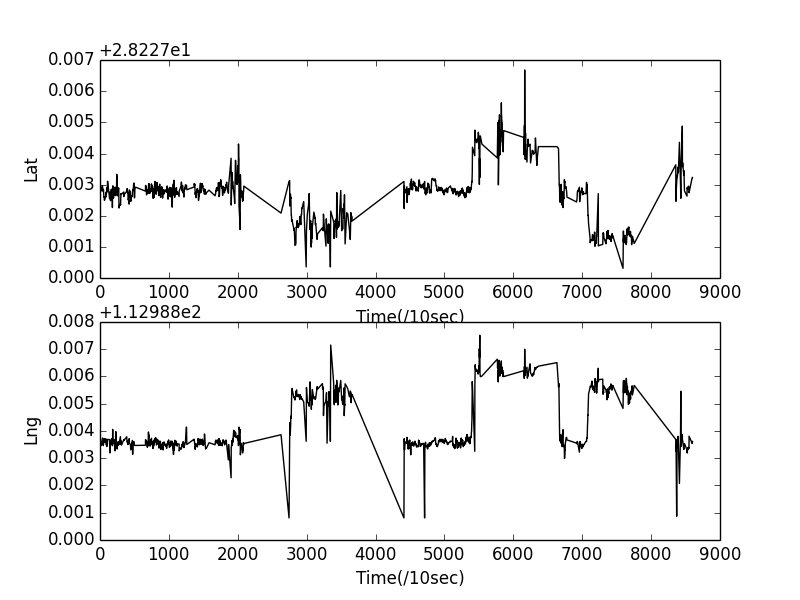
\includegraphics[height=4cm]{figure3_2_2_1}}\hspace{4em}%
  \subfloat[卡尔曼滤波]{%
    \label{fig:3_2_2_2}
    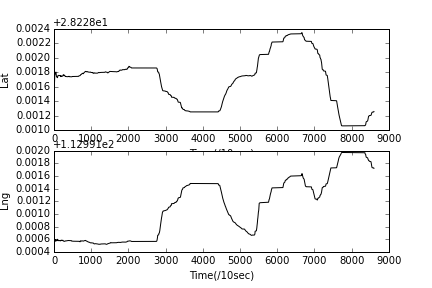
\includegraphics[height=4cm]{figure3_4_2_2}}
  \caption{卡尔曼滤波实验结果3-2}
  \label{fig:3_4_2}
\end{figure}
\begin{figure}[htb]
  \centering%
  \subfloat[原始数据]{%
    \label{fig:3_2_3_1}
    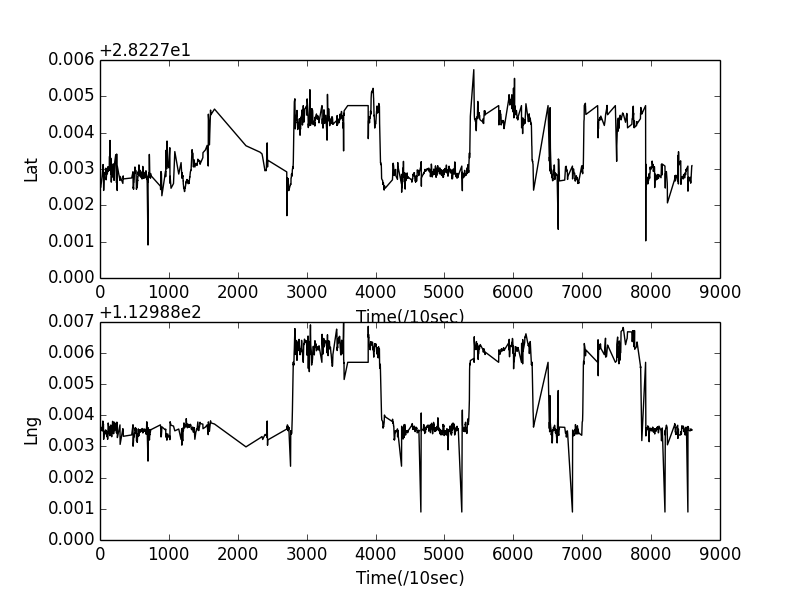
\includegraphics[height=4cm]{figure3_2_3_1}}\hspace{4em}%
  \subfloat[卡尔曼滤波]{%
    \label{fig:3_2_3_2}
    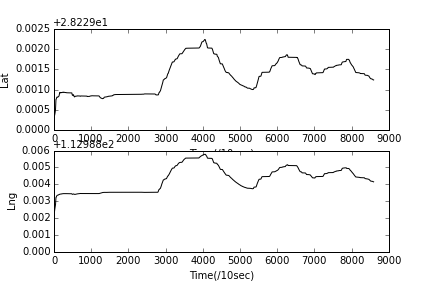
\includegraphics[height=4cm]{figure3_4_3_2}}
  \caption{卡尔曼滤波实验结果3-3}
  \label{fig:3_4_3}
\end{figure}
\par 卡尔曼滤波的结果虽然更加平滑,但是通过分析实验结果发现,滤波结果严重损坏了原来的信息,使得整个轨迹曲线趋于常数值。经过更深一步的分析发现,用户每天的轨迹只有在某些固定位置(即后文所说的语义位置)时会在一段时间内保持不变,因此采用一些简单的方法对每天的轨迹进行划分,尽可能使每段轨迹中的点都采样自某一个固定位置,然后对这一段轨迹进行卡尔曼滤波,肯定能够得到一个更好的滤波结果。
\par 本课题采用一些非常简单且容易实现的方法对轨迹进行分段。如果在一段时间内,任意相邻两个采样点之间时间间隔不超过十分钟(超过十分钟用户位置就很可能发生变化,十分钟是一个参数值,也可以根据实际情况进行调节),任意两个采样点之间真实距离不超过20米,则认为这段时间内所有的采样点属于一个片段。采用贪心的思想寻找满足上述两个条件的序列,即如果加入下一个点,不破坏上述两个条件,则当前序列应该包含下一个点,如果加入下一个点后,上述两个条件之一或全部被破坏,则当前序列为当天轨迹的一个片段,且不包含下一个点。下文展示分段处理后卡尔曼滤波的结果,见图\ref{fig:3_5_1}、\ref{fig:3_5_2}、\ref{fig:3_5_3}。
\begin{figure}[htb]
  \centering%
  \subfloat[原始数据]{%
    \label{fig:3_2_1_1}
    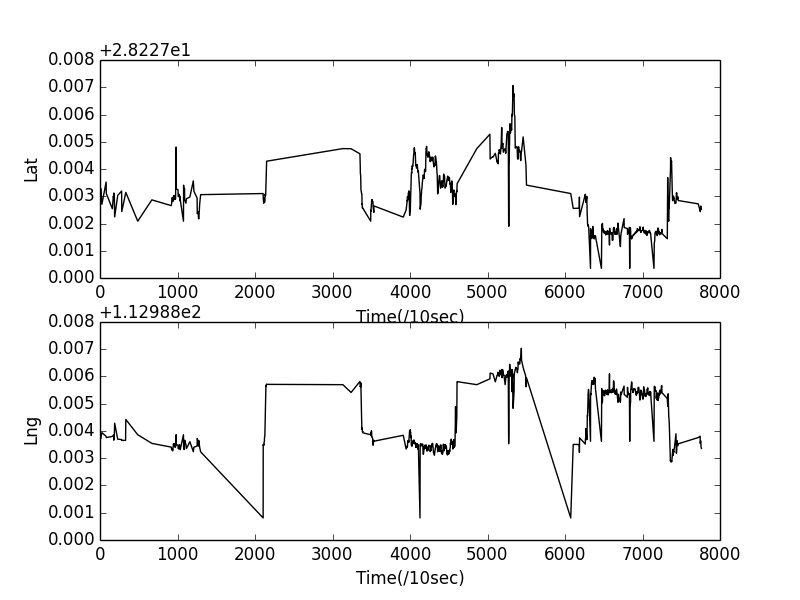
\includegraphics[height=4cm]{figure3_2_1_1}}\hspace{4em}%
  \subfloat[分段卡尔曼滤波]{%
    \label{fig:3_2_2_1}
    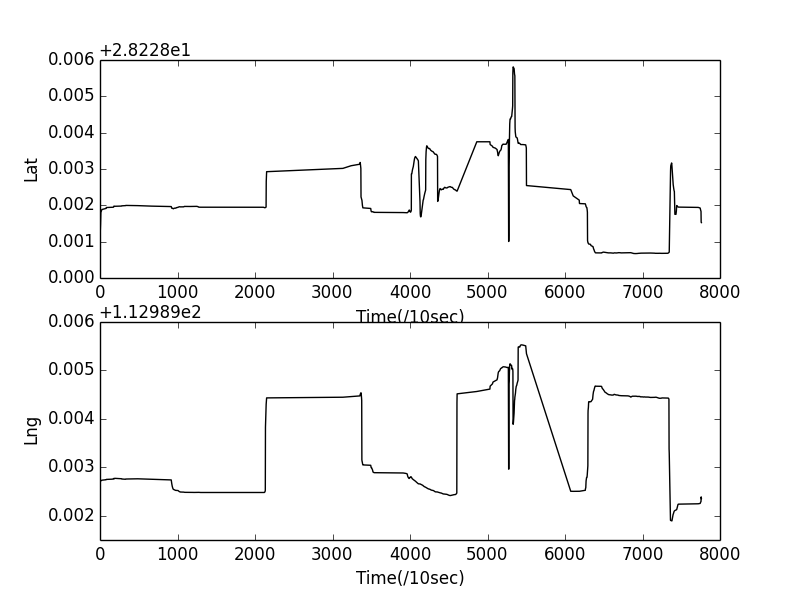
\includegraphics[height=4cm]{figure3_5_1_2}}
  \caption{分段卡尔曼滤波实验结果3-1}
  \label{fig:3_5_1}
\end{figure}
\begin{figure}[htb]
  \centering%
  \subfloat[原始数据]{%
    \label{fig:3_2_2_1}
    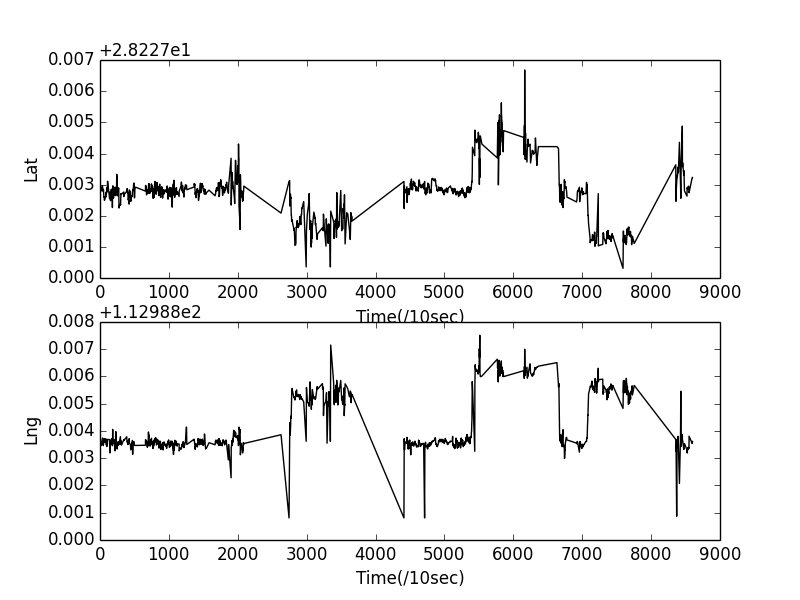
\includegraphics[height=4cm]{figure3_2_2_1}}\hspace{4em}%
  \subfloat[分段卡尔曼滤波]{%
    \label{fig:3_2_2_2}
    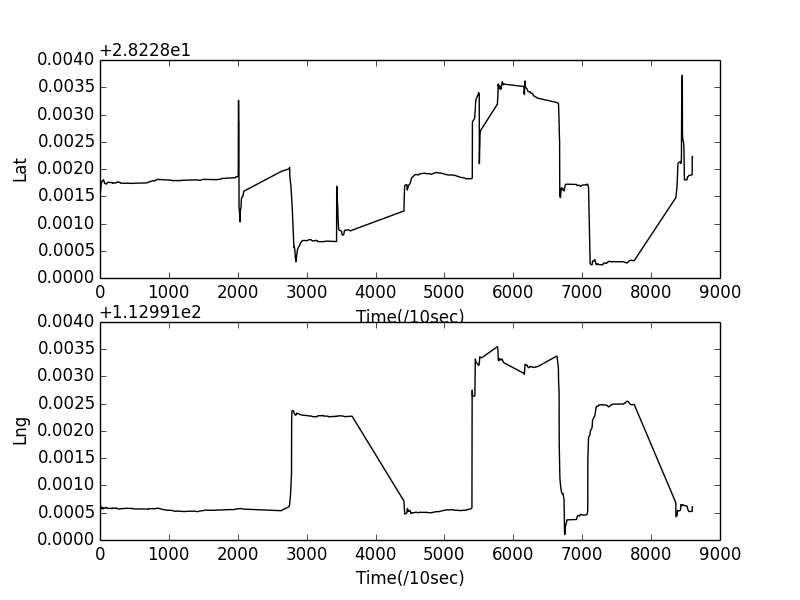
\includegraphics[height=4cm]{figure3_5_2_2}}
  \caption{分段卡尔曼滤波实验结果3-2}
  \label{fig:3_5_2}
\end{figure}
\begin{figure}[htb]
  \centering%
  \subfloat[原始数据]{%
    \label{fig:3_2_3_1}
    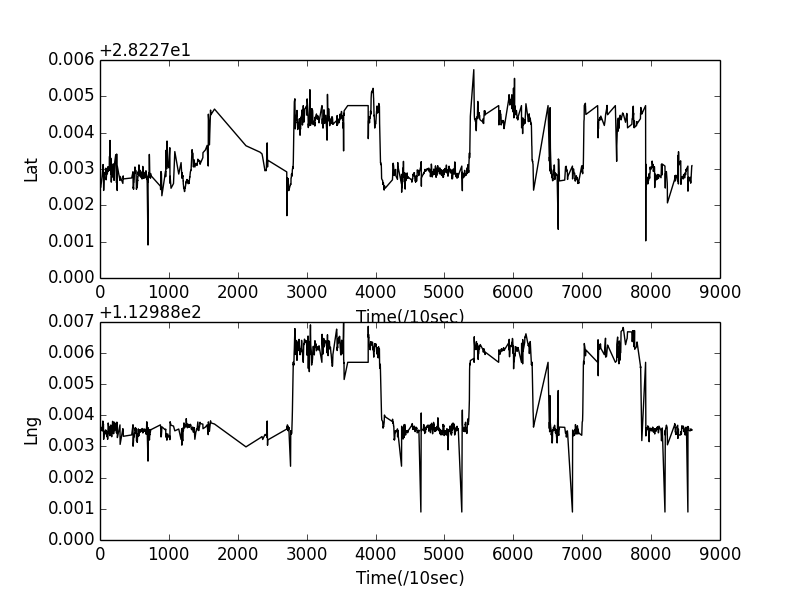
\includegraphics[height=4cm]{figure3_2_3_1}}\hspace{4em}%
  \subfloat[分段卡尔曼滤波]{%
    \label{fig:3_2_3_2}
    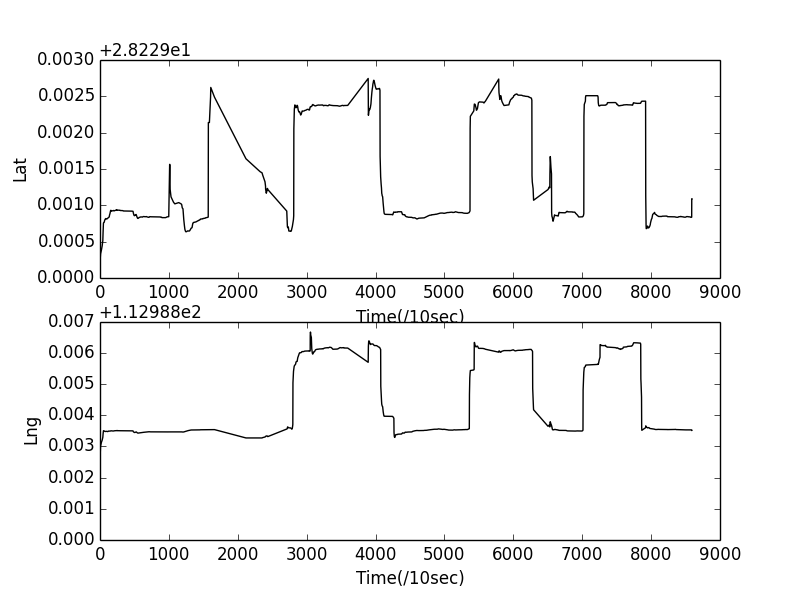
\includegraphics[height=4cm]{figure3_5_3_2}}
  \caption{分段卡尔曼滤波实验结果3-3}
  \label{fig:3_5_3}
\end{figure}
\par 这一小节主要描述了均值滤波,中值滤波、卡尔曼滤波以及分段卡尔曼滤波的实验结果,通过实验发现分段卡尔曼滤波的结果更加平滑,更符合实际情况。下一小节将描述如何剔除路上的点。
\subsection{剔除路上的点}
在现实生活中,人们从一个位置行进到另一个位置是连续的,即采集的数据必然存在很多路上的点。而这些路上的点不属于任何一个语义位置。且在分析关系强度时,如果两个人同时来到同一个语义位置,但是一个从某一个方向过来,而另一个从相反方向过来,虽然这两个人其实在这段时间内待在同一个地方,如果不剔除路上的点,则这两个人的物理位置会受到路上的点的影响,从而使得这两个人轨迹的空间距离反而比较大。在上文讨论的降噪过程中,已经处理了误差比较大的点,因此本节主要讨论如何剔除路上的点。
\par 仔细分析路上的点的特性,发现人们通常在语义位置停留时间比较长,而在路上一直处于移动状态,所以路上点密度通常远远小于语义位置的点的密度。密度定义见公式\ref{equ:chap2:dj-cluster}。且在实际生活中,在路上时通常处于移动状态,设速度为$v$,且每条路每天走的次数也存在上限,设每条路每天最多走$N$ 次,计算密度时采用的半径参数为$R$,设GPS采样频率为$f$。 因为半径参数很小,故可视为在该半径对应圆形区域中行走路线为直线。路上点的密度D存在最大值,计算方法见公式\ref{equ:chap3:density_01}。因此本文采用基于密度的方法剔除异常点。该方法的基本思想为若某个点的密度小于给定阈值,则该点为异常点。通过对日常数据的分析发现,路上点的密度确实远远小于处于语义位置点的密度,见图\ref{figure3_6}。
\begin{equation}
\label{equ:chap3:density_01}
D=N \ast \frac{2R}{v} \ast f
\end{equation}
\begin{figure}[htp]
\centering
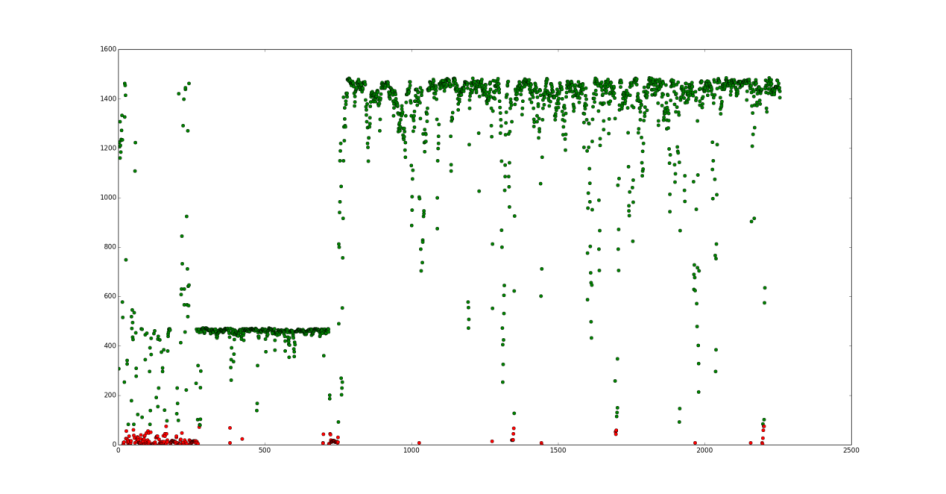
\includegraphics[width=6in]{figure3_6}
\caption{绿色表示正常点,红色表示路上的点}
\label{fig:3_6}
\end{figure}
\par 根据上下文的分析,可以计算出密度的上限值,假设计算密度时的半径设为10米,每天经过这条路4次,步行速度约为80 米每分钟,这样每个点的密度的上限值大概是60。同时本课题研究发现有一种方法可以自动学习参数,后文将会对比学习到的密度上限值和计算值的异同。
\par 假设对于某一天的数据,已经聚好类,即我们知道哪一个点属于哪一个类别,仔细分析每个路上的点对类别中心的影响,假设用户在某个地方时处于某一个固定的位置,GPS采样因为采样误差服从高斯分布,因此大多数点都处在该固定位置对应实际点(可能是类别中心,非常有可能在类别中心附近)的周围。而路上的点会距离实际点比较远,因此,该类别所有点到类别中心的距离的平均值会被路上的点拉大,如果逐渐提高密度的上限值,从而有更多的点因为密度小而被删除,讨论一种理想情况,如果路上的点完全被剔除,剩下的点都是实际点加高斯误差,因为实际点大量存在,使得即使我们剔除一小部分实际点,对该类别所有点到类别中心的距离的平均值也不会产生太大的影响。所以可以从一个很小的密度上限值逐渐增加,剔除小于该密度的点之后计算对应的平均距离,若平均距离收敛,则认为这个密度值是路上的点的密度的上限值。平均距离的定义见公式\ref{equ:chap3:avgdis_01},其中$p_{ij}$为第$i$类第$j$个点,$c_{i}$为第$i$类的类别中心,$dis(a,b)$表示$a$和$b$之间的距离,$n_{i}$为第$i$类点的个数,$k$为类别的个数,$N$为所有点的个数。使用连续四天采集的数据做了实验,计算其平均距离,见图\ref{fig:3_7}。
\begin{equation}
\label{equ:chap3:avgdis_01}
AvgDis=\frac{\sum_{i=1}^{k}\sum_{j=1}^{n_{i}}dis(p_{ij},c_{i})}{N}
\end{equation}
\begin{figure}[htb]
  \centering%
  \subfloat[第一天数据]{%
    \label{fig:3_7_1}
    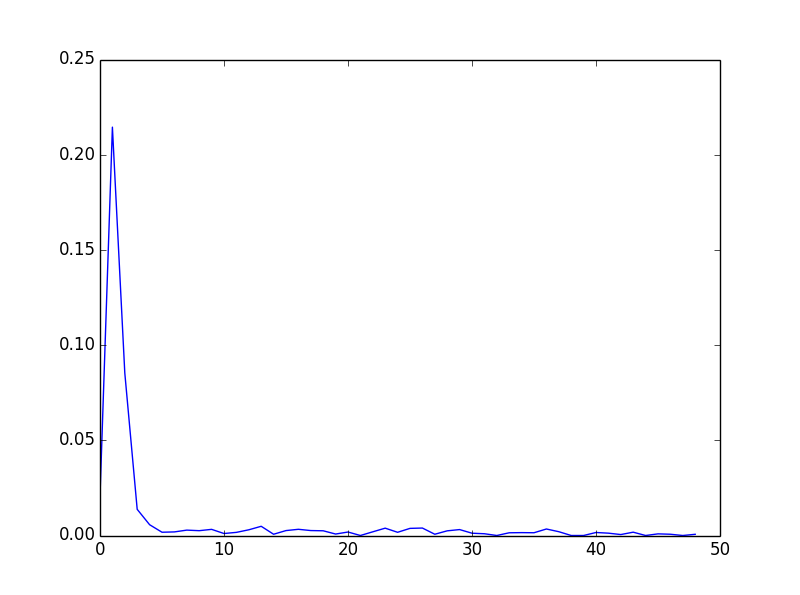
\includegraphics[height=5cm]{figure3_7_1}}%\hspace{4em}
  \subfloat[第二天数据]{%
    \label{fig:3_7_2}
    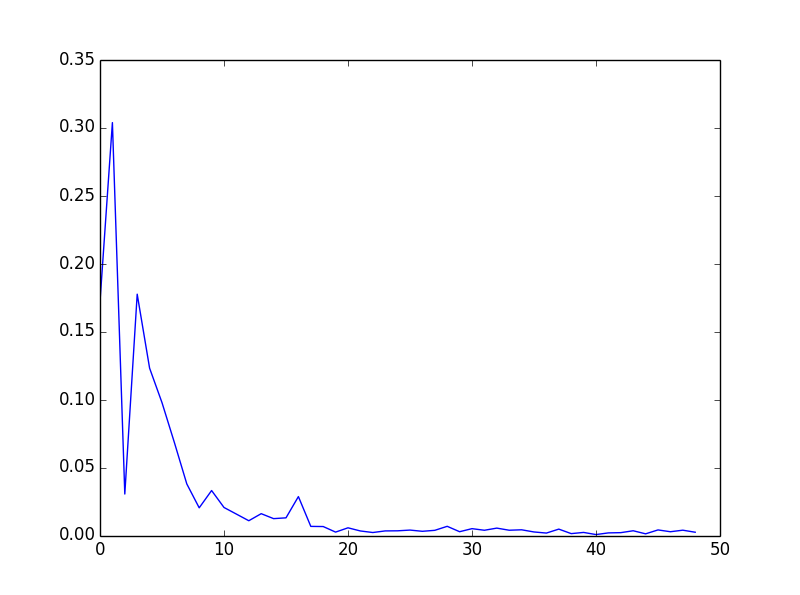
\includegraphics[height=5cm]{figure3_7_2}}\\
  \subfloat[第三天数据]{%
    \label{fig:3_7_3}
    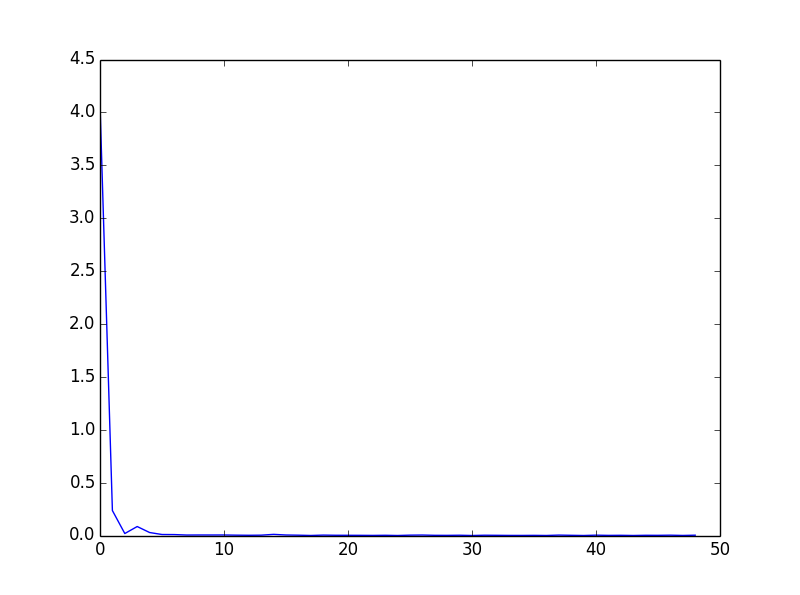
\includegraphics[height=5cm]{figure3_7_3}}
  \subfloat[第四天数据]{%
    \label{fig:3_7_4}
    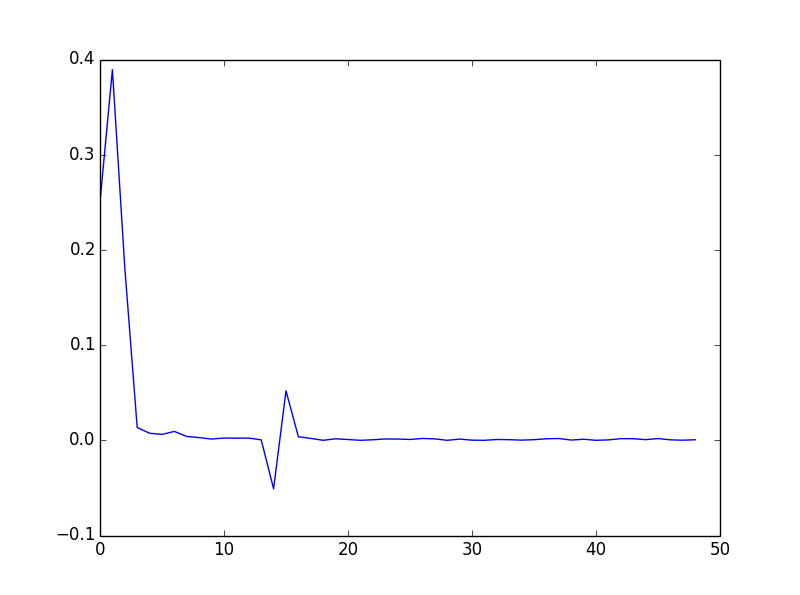
\includegraphics[height=5cm]{figure3_7_4}}
  \caption{平均距离收敛}
  \label{fig:3_7}
\end{figure}
\par 通过观察图\ref{fig:3_7},发现密度上限值大概是40到50之间,前文计算的密度上限值是60左右,一方面因为两种计算方法都存在一定的误差,另一方面是在实际过程中,手机并不是持续高频采样,经常会因为各种各样的原因而丢失一些采样点。在实际应用中,可以先手动处理某一天的数据,然后使用该自动学习的算法学习到密度的上限值,从而用作其他天数据处理的参数。
\par 这一小节主要讨论了如何剔除路上的点,以及如何学习路上点的密度的上限值,下一小节将通过实验讨论K-MEANS、DJ-cluster、以及Science上发表算法三种聚类算法的优缺点,以及在实际数据上应用的效果。
\subsection{聚类得到语义位置}
这一小节将重点描述使用聚类算法得到语义位置时,不同算法以及不同参数对结果产生的影响。K-MEANS、DJ-Cluster以及Science 上发表的三个算法算法原理在第二章已经描述过了,下文将通过实验依次展示三个算法对相同数据聚类得到的结果。数据使用文献\cite{rawassizadeh2013ubiqlog}中的采集工具采集。
\par 首先展示K-MEANS聚类算法的实验结果,K-MEANS聚类算法的主要缺点有两个:一个是需要预知类别的个数;另一个是同一类别的数据最好是团状或簇状。对于本课题研究的问题而言,通常遇到的建筑都是每栋楼占单独的一块地方,相邻建筑一般都会有一定的间隔,因此K-MEANS聚类算法的第二个缺点因为本课题研究的具体问题而不复存在,故主要考虑不同类别个数对实验结果的影响。图\ref{fig:3_8_1}、\ref{fig:3_8_2}、\ref{fig:3_8_3} 主要展示了不同参数对K-MEANS聚类结果的影响。图\ref{fig:3_9_1}、\ref{fig:3_9_2}、\ref{fig:3_9_3}在地图上标记了不同参数聚类得到的聚类中心。
\begin{figure}[htb]
  \centering%
  \subfloat[原始数据]{%
    \label{fig:3_8_1_1}
    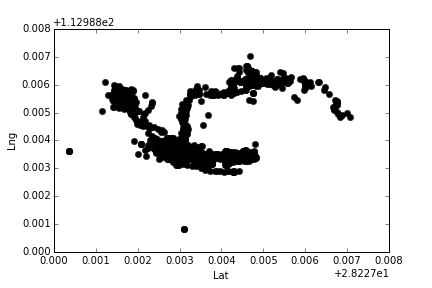
\includegraphics[height=5cm]{figure3_8_1_1}}%\hspace{4em}
  \subfloat[k=3]{%
    \label{fig:3_8_1_2}
    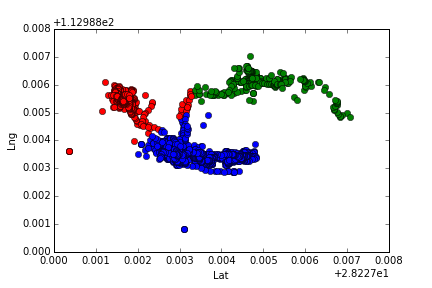
\includegraphics[height=5cm]{figure3_8_1_2}}\\
  \subfloat[k=4]{%
    \label{fig:3_8_1_3}
    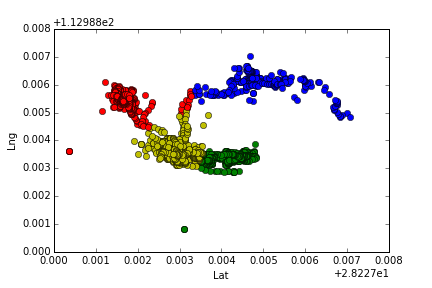
\includegraphics[height=5cm]{figure3_8_1_3}}
  \subfloat[k=5]{%
    \label{fig:3_8_1_4}
    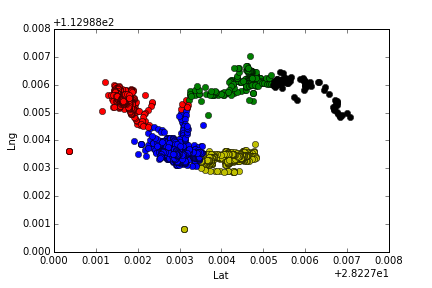
\includegraphics[height=5cm]{figure3_8_1_4}}
  \caption{K-MEANS聚类实验结果3-1}
  \label{fig:3_8_1}
\end{figure}
\begin{figure}[htb]
  \centering%
  \subfloat[原始数据]{%
    \label{fig:3_9_1_1}
    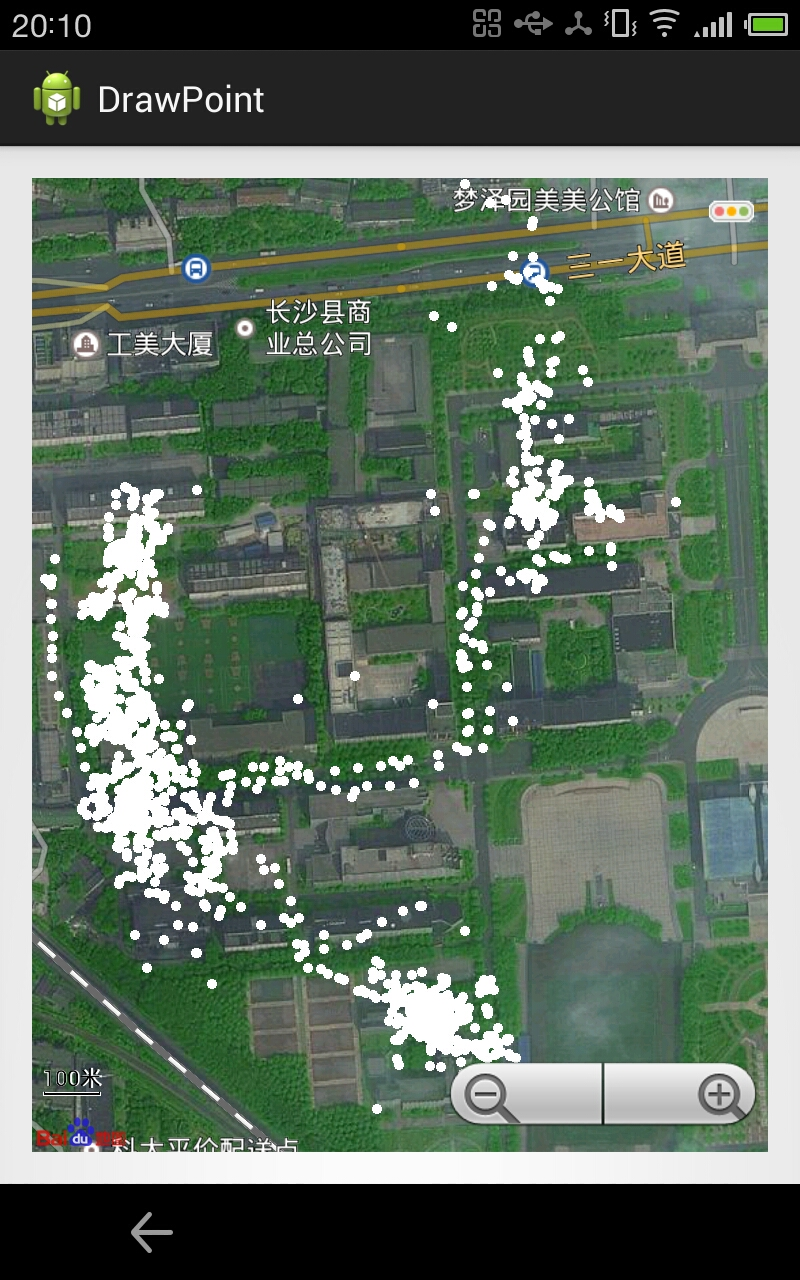
\includegraphics[height=6cm]{figure3_9_1_1}}%\hspace{4em}
  \subfloat[k=3]{%
    \label{fig:3_9_1_2}
    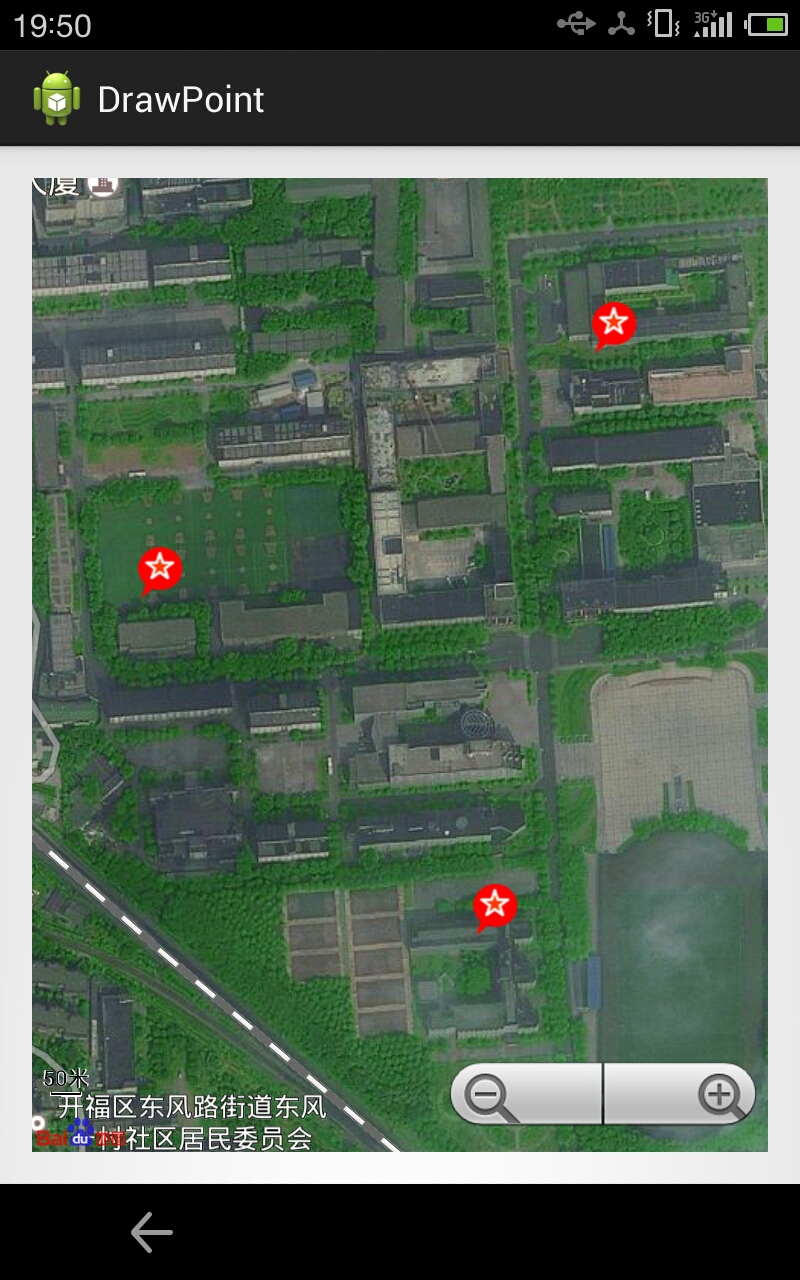
\includegraphics[height=6cm]{figure3_9_1_2}}
  \subfloat[k=4]{%
    \label{fig:3_9_1_3}
    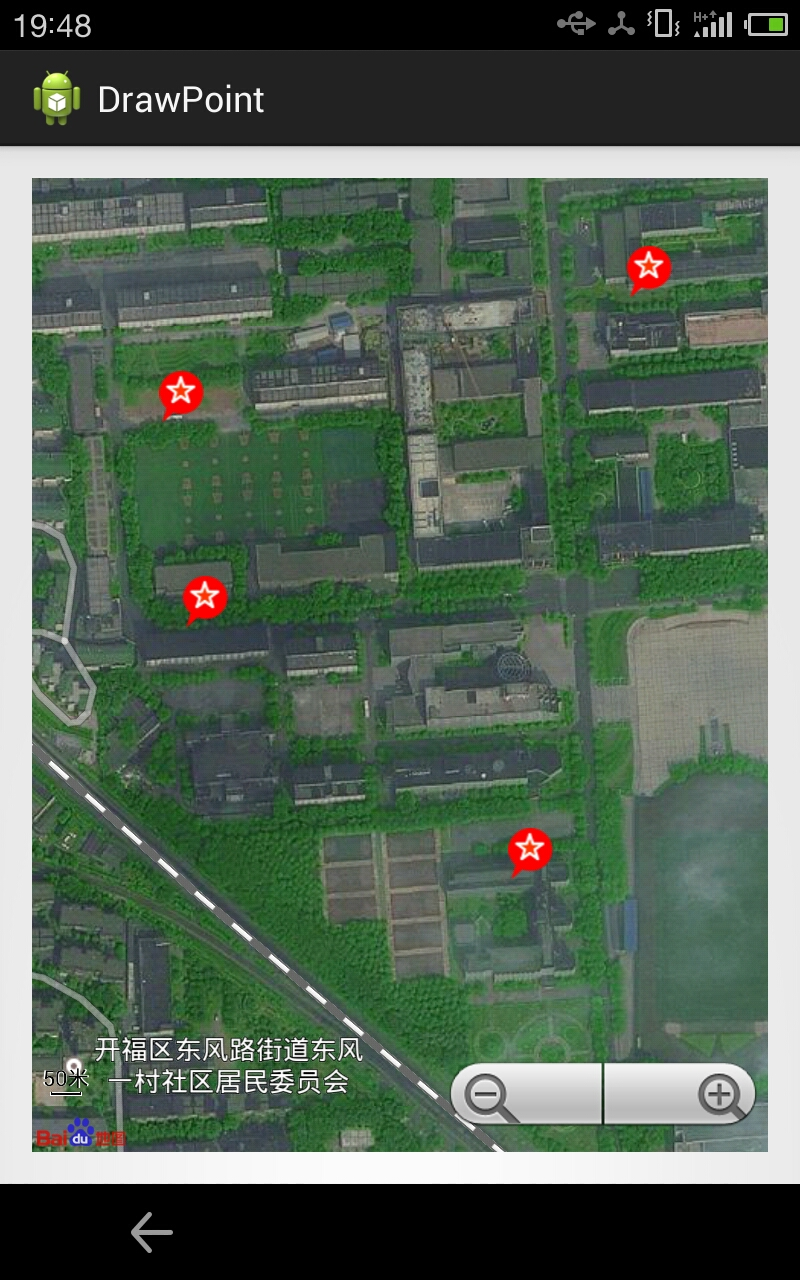
\includegraphics[height=6cm]{figure3_9_1_3}}
  \subfloat[k=5]{%
    \label{fig:3_9_1_4}
    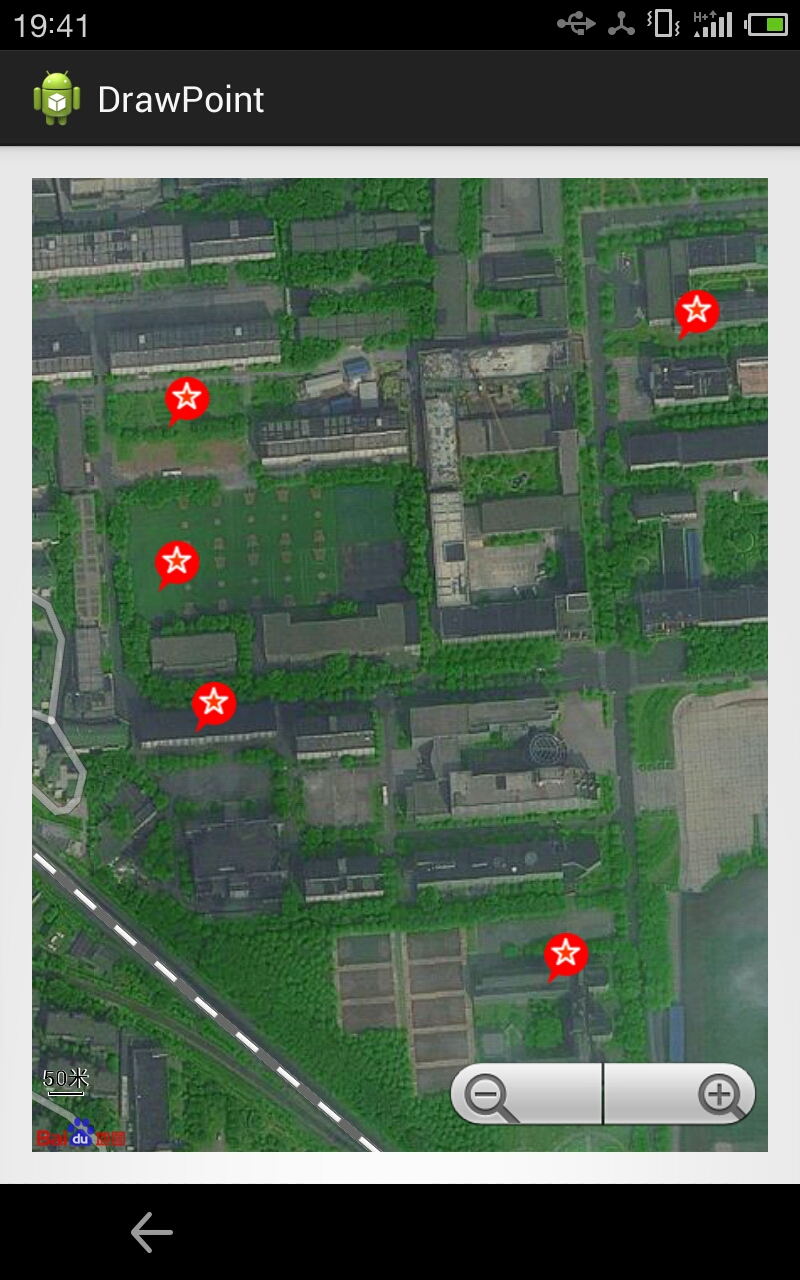
\includegraphics[height=6cm]{figure3_9_1_4}}
  \caption{K-MEANS聚类实验结果地图展示3-1}
  \label{fig:3_9_1}
\end{figure}
\begin{figure}[htb]
  \centering%
  \subfloat[原始数据]{%
    \label{fig:3_8_2_1}
    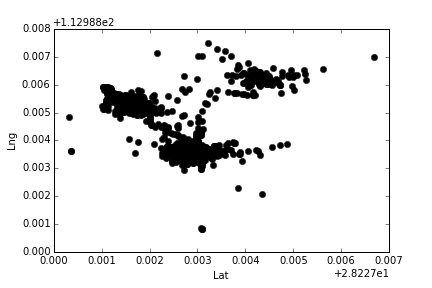
\includegraphics[height=5cm]{figure3_8_2_1}}%\hspace{4em}
  \subfloat[k=3]{%
    \label{fig:3_8_2_2}
    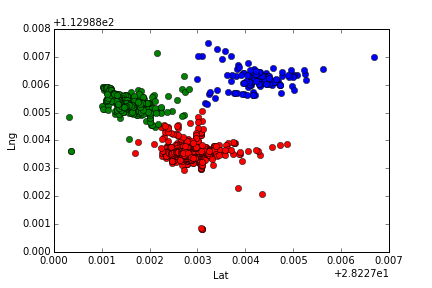
\includegraphics[height=5cm]{figure3_8_2_2}}\\
  \subfloat[k=4]{%
    \label{fig:3_8_2_3}
    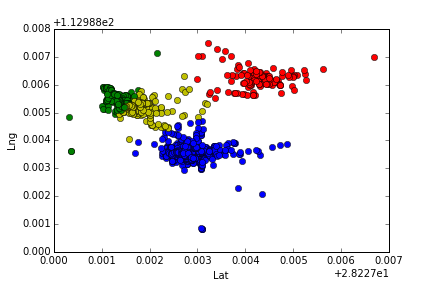
\includegraphics[height=5cm]{figure3_8_2_3}}
  \subfloat[k=5]{%
    \label{fig:3_8_2_4}
    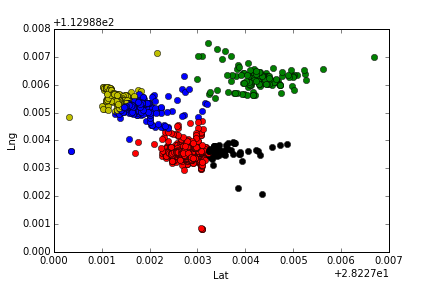
\includegraphics[height=5cm]{figure3_8_2_4}}
  \caption{K-MEANS聚类实验结果3-2}
  \label{fig:3_8_2}
\end{figure}
\begin{figure}[htb]
  \centering%
  \subfloat[原始数据]{%
    \label{fig:3_9_2_1}
    \includegraphics[height=6cm]{figure3_9_2_1}}%\hspace{4em}
  \subfloat[k=3]{%
    \label{fig:3_9_2_2}
    \includegraphics[height=6cm]{figure3_9_2_2}}
  \subfloat[k=4]{%
    \label{fig:3_9_2_3}
    \includegraphics[height=6cm]{figure3_9_2_3}}
  \subfloat[k=5]{%
    \label{fig:3_9_2_4}
    \includegraphics[height=6cm]{figure3_9_2_4}}
  \caption{K-MEANS聚类实验结果地图展示3-2}
  \label{fig:3_9_2}
\end{figure}
\begin{figure}[htb]
  \centering%
  \subfloat[原始数据]{%
    \label{fig:3_8_3_1}
    \includegraphics[height=5cm]{figure3_8_3_1}}%\hspace{4em}
  \subfloat[k=3]{%
    \label{fig:3_8_3_2}
    \includegraphics[height=5cm]{figure3_8_3_2}}\\
  \subfloat[k=4]{%
    \label{fig:3_8_3_3}
    \includegraphics[height=5cm]{figure3_8_3_3}}
  \subfloat[k=5]{%
    \label{fig:3_8_3_4}
    \includegraphics[height=5cm]{figure3_8_3_4}}
  \caption{K-MEANS聚类实验结果3-3}
  \label{fig:3_8_3}
\end{figure}
\begin{figure}[htb]
  \centering%
  \subfloat[原始数据]{%
    \label{fig:3_9_3_1}
    \includegraphics[height=6cm]{figure3_9_3_1}}%\hspace{4em}
  \subfloat[k=2]{%
    \label{fig:3_9_3_2}
    \includegraphics[height=6cm]{figure3_9_3_2}}
  \subfloat[k=3]{%
    \label{fig:3_9_3_3}
    \includegraphics[height=6cm]{figure3_9_3_3}}
  \subfloat[k=4]{%
    \label{fig:3_9_3_4}
    \includegraphics[height=6cm]{figure3_9_3_4}}
  \caption{K-MEANS聚类实验结果地图展示3-3}
  \label{fig:3_9_3}
\end{figure}
\par 仔细分析这三组数据的实验结果发现,如果能够预先知道类别的个数,K-MEANS算法确实能够得到一个非常好的结果,特别对于图\ref{fig:3_9_2},仔细观察(a)对应的原始数据,地图右下角白色点群表明其实去了两个教学楼,但是两个教学楼距离太近以及GPS本身存在的采样误差使得采样点混合在一起。如果假设去了三个地方时,该聚类算法将两个教学楼识别成了一个位置,如果假设去了四个地方时,聚类算法成功的区分了这两个实验楼,在另外两个算法的实验中将发现,另外两个算法无法区分这两个实验楼。对于图\ref{fig:3_9_1},其实只参观了三个地方,但是如果假设去了四个地方,该聚类算法也能将数据分成四类,仔细观察得到第四个类别其实是两条路的交叉点,从另一个角度证明前文论述应该剔除路上的点是非常合理的,而后文的实验也证明剔除路上的点之后,聚类算法就不会再把路上的点识别成聚类中心。
\par 下文将展示DJ-Cluster算法的实验结果,DJ-Cluster是基于DBSCAN算法的一种基于密度的聚类算法,通过边界点将相邻类别合并从而使得算法对参数更加鲁棒。但是算法本身仍然严重依赖半径值和密度值这两个参数,在实际应用过程中,仍然需要仔细调节参数,在参数设置理想的情况下,仍然能够得到非常理想的结果,见图\ref{fig:3_10_1}、\ref{fig:3_10_2}、\ref{fig:3_10_3},其地图表示见图\ref{fig:3_11_1}、\ref{fig:3_11_2}、\ref{fig:3_11_3}。
\begin{figure}[htb]
  \centering%
  \subfloat[原始数据]{%
    \label{fig:3_10_1_1}
    \includegraphics[height=4cm]{figure3_8_1_1}}\hspace{4em}%
  \subfloat[聚类结果]{%
    \label{fig:3_10_1_2}
    \includegraphics[height=4cm]{figure3_10_1_2}}
  \caption{DJ-Cluster实验结果3-1}
  \label{fig:3_10_1}
\end{figure}
\begin{figure}[htb]
  \centering%
  \subfloat[原始数据]{%
    \label{fig:3_11_1_1}
    \includegraphics[height=6cm]{figure3_9_1_1}}\hspace{4em}%
  \subfloat[聚类结果]{%
    \label{fig:3_11_1_2}
    \includegraphics[height=6cm]{figure3_11_1_2}}
  \caption{DJ-Cluster实验结果地图表示3-1}
  \label{fig:3_11_1}
\end{figure}
\begin{figure}[htb]
  \centering%
  \subfloat[原始数据]{%
    \label{fig:3_10_2_1}
    \includegraphics[height=4cm]{figure3_8_2_1}}\hspace{4em}%
  \subfloat[聚类结果]{%
    \label{fig:3_10_2_2}
    \includegraphics[height=4cm]{figure3_10_2_2}}
  \caption{DJ-Cluster实验结果3-2}
  \label{fig:3_10_2}
\end{figure}
\begin{figure}[htb]
  \centering%
  \subfloat[原始数据]{%
    \label{fig:3_11_2_1}
    \includegraphics[height=6cm]{figure3_9_2_1}}\hspace{4em}%
  \subfloat[聚类结果]{%
    \label{fig:3_11_2_2}
    \includegraphics[height=6cm]{figure3_11_2_2}}
  \caption{DJ-Cluster实验结果地图表示3-2}
  \label{fig:3_11_2}
\end{figure}
\begin{figure}[htb]
  \centering%
  \subfloat[原始数据]{%
    \label{fig:3_10_3_1}
    \includegraphics[height=4cm]{figure3_8_3_1}}\hspace{4em}%
  \subfloat[聚类结果]{%
    \label{fig:3_10_3_2}
    \includegraphics[height=4cm]{figure3_10_3_2}}
  \caption{DJ-Cluster实验结果3-3}
  \label{fig:3_10_3}
\end{figure}
\begin{figure}[htb]
  \centering%
  \subfloat[原始数据]{%
    \label{fig:3_11_3_1}
    \includegraphics[height=6cm]{figure3_9_3_1}}\hspace{4em}%
  \subfloat[聚类结果]{%
    \label{fig:3_11_3_2}
    \includegraphics[height=6cm]{figure3_11_3_2}}
  \caption{DJ-Cluster实验结果地图表示3-3}
  \label{fig:3_11_3}
\end{figure}
\par 通过对实验结果的分析能够发现,DJ-Cluster基本上能够得到一个令人满意的结果,在仔细调节参数后,基本上识别出了所有的位置,但是图\ref{fig:3_11_2}右下角其实是两个教学楼,前文已经论述过,DJ-Cluster将其识别为一个位置,主要是因为这两个教学楼本身距离太小,且GPS采样误差比较大使得本来分属于两栋楼的采样点有重合,从而使得基于密度的方法无法区分。除此情况外,对于另外两天的数据,该算法都表现出了非常好的识别结果。该算法最大的缺陷还是对参数比较敏感,下文将介绍Science 发表的聚类算法的实验结果,同时会从算法原理上简要论述其对参数的鲁棒性确实优于DJ-Cluster。
\par 下文描述Science发表的聚类算法对应的实验结果,在描述具体实验之前,首先分析该算法的原理:该算法对每个点计算对应的密度(密度定义见前文),对所有点按密度排序;然后计算每个点的距离,再对每个点按距离和密度的乘积排序得到最终的聚类结果。DJ-Cluster算法之所以对参数敏感是因为不同的半径值就需要对应不同的密度值(半径大了,此半径对应的圆形区域内其他点的数目肯定会更多),而Science发表的算法会对所有点按密度排序,这样在很大程度上降低了半径值对算法本身的影响,通常情况下半径越大点密度越大,如果随着半径的增长,密度的相对顺序保持不变,则半径对该算法基本没有影响,本课题收集的GPS 采样点基本满足这一条件,若某个点在小半径时密度小,则在大半径是其密度依然相对较小。所以Science发表的算法对当前问题而言有非常好的鲁棒性。具体的实验结果见图\ref{fig:3_12_1}、\ref{fig:3_12_2}、\ref{fig:3_12_3}。实验结果地图表示见图\ref{fig:3_13_1}、\ref{fig:3_13_2}、\ref{fig:3_13_3}。
\begin{figure}[htb]
  \centering%
  \subfloat[原始数据]{%
    \label{fig:3_12_1_1}
    \includegraphics[height=4cm]{figure3_8_1_1}}\hspace{4em}%
  \subfloat[聚类结果]{%
    \label{fig:3_12_1_2}
    \includegraphics[height=4cm]{figure3_12_1_2}}
  \caption{Science发表算法实验结果3-1}
  \label{fig:3_12_1}
\end{figure}
\begin{figure}[htb]
  \centering%
  \subfloat[原始数据]{%
    \label{fig:3_13_1_1}
    \includegraphics[height=6cm]{figure3_9_1_1}}\hspace{4em}%
  \subfloat[聚类结果]{%
    \label{fig:3_13_1_2}
    \includegraphics[height=6cm]{figure3_13_1_2}}
  \caption{Science发表算法实验结果地图表示3-1}
  \label{fig:3_13_1}
\end{figure}
\begin{figure}[htb]
  \centering%
  \subfloat[原始数据]{%
    \label{fig:3_12_2_1}
    \includegraphics[height=4cm]{figure3_8_2_1}}\hspace{4em}%
  \subfloat[聚类结果]{%
    \label{fig:3_12_2_2}
    \includegraphics[height=4cm]{figure3_12_2_2}}
  \caption{Science发表算法实验结果3-2}
  \label{fig:3_12_2}
\end{figure}
\begin{figure}[htb]
  \centering%
  \subfloat[原始数据]{%
    \label{fig:3_13_2_1}
    \includegraphics[height=6cm]{figure3_9_2_1}}\hspace{4em}%
  \subfloat[聚类结果]{%
    \label{fig:3_13_2_2}
    \includegraphics[height=6cm]{figure3_13_2_2}}
  \caption{Science发表算法实验结果地图表示3-2}
  \label{fig:3_13_2}
\end{figure}
\begin{figure}[htb]
  \centering%
  \subfloat[原始数据]{%
    \label{fig:3_12_3_1}
    \includegraphics[height=4cm]{figure3_8_3_1}}\hspace{4em}%
  \subfloat[聚类结果]{%
    \label{fig:3_12_3_2}
    \includegraphics[height=4cm]{figure3_12_3_2}}
  \caption{Science发表算法实验结果3-3}
  \label{fig:3_12_3}
\end{figure}
\begin{figure}[htb]
  \centering%
  \subfloat[原始数据]{%
    \label{fig:3_13_3_1}
    \includegraphics[height=6cm]{figure3_9_3_1}}\hspace{4em}%
  \subfloat[聚类结果]{%
    \label{fig:3_13_3_2}
    \includegraphics[height=6cm]{figure3_13_3_2}}
  \caption{Science发表算法实验结果地图表示3-3}
  \label{fig:3_13_3}
\end{figure}
\par 仔细分析由Science发表算法对应的实验结果发现,其结果和DJ-Cluster的结果基本完全一致,图\ref{fig:3_13_2}、其实有四个地方,该算法也只识别出来三个,未能正确识别的原因如前文所述,其对另外两天的数据都能全部识别出来。其算法的鲁棒性在前文已经论述过了,在此讨论与该算法相关的另外一个参数,即密度和距离乘积的阈值。原论文中声明他们的算法不需要任何手动设置任何参数,但是经过实验发现该阈值仍然需要通过观察具体数据集的特性来确定。虽然不能完全不需要人的参与,通过实验发现对于特定的数据集,比如采集的校园内的GPS数据,通过对第一天数据的分析,能够得到一个密度和距离乘积的阈值,通过实验发现该阈值对后面采集的数据依然有效,即只需要在刚开始使用该算法时确定该参数,就可以使用该参数处理其他剩余的数据。这样在很大程度上减少了人与机器的交互,使得该算法更加实用。
\par 这一小节主要讨论了三种聚类算法以及不同的参数对实验结果的影响。最后讨论对每天数据进行聚类的优缺点。以前的工作都是采集一段时间的数据,把所有数据合并到一起,然后用这些聚类算法来计算对应的语义位置。最明显的一个问题是如果聚类结果表明这些数据总共产生了1000个位置(如果是K-MEANS 算法需要预先设定类别的个数),那么这些数据是否恰好对应1000个语义位置。这样做的优点是处理方便,只需要一次交互,缺点是计算结果无法验证。当然,主要是因为移动感知这个领域目前对结果精度要求也不是很高,但是有没有什么办法在不明显增加处理复杂度的同时使得结果更加精确?因此本课题决定对每天的数据进行聚类,一方面小数据更容易精确识别,如果用户总共去了三个地方,可能识别出来两个,则只有一个没有识别出来,而没事别出来的那个可能因为下文论述的原因被重新发现,如果把所有数据一起处理,假设总共参观了100个地方,可能只识别出来70几个,另外20 多个无法被识别;另一方面如果每个地方因为当天采集数据太少而未被识别,用户下一次去这个地方且采集数据较多时就会被重新识别出来,对最终结果来说,仍然正确识别了这个地方。而且小数据量使得在移动端计算成为可能,可以将整个过程全部放在手机上,而不影响用户体验。在识别出这些位置后下一步需要标记其语义标签,将大量的数据分散到每天,且通过识别新的位置以及对新位置计算可能的语义标签在很大程度上降低了用户与手机的交互,下一节将详细讨论如何在发现语义位置后对其标记对应的语义标签。
\section{对语义位置标语义标签}
\label{sec:section3-3}
在上一节主要描述了如何对GPS数据进行滤波以达到降噪的目的、如何剔除路上的点以及如何使用聚类算法得到语义位置。仅仅得到语义位置的信息是不够的,如果只是知道这个用户在什么时候去了一个地方,但是并不知道这个地方是什么(一般指该地方的功名称)。如果能够得到这个地方的语义信息,则能够解决更多的问题。如果知道一个人从早到晚一整天都在实验室,只使用这些信息就可以确定,这个人很大可能是博士。而且根据用户经常停留的位置也可以从健康角度提一些建议,如果某用户整天在室内办公,就可以提醒他应该抽出一定的时间去室外锻炼。因此,确定语义位置对应的语义标签是非常重要的一个问题。本节主要介绍如何确定语义位置对应的语义标签。
\subsection{发现新位置}
一般通过两种方法来得到语义位置对应的语义标签。一种方法是预先定义几种语义标签,使用监督学习的方法学习出一个分类器模型,然后对未知标签的数据通过用分类器分类得到其对应的语义标签。该方法的优点是结果比较准确,有坚实的理论基础做支撑,而且只有在收集数据时需要用户参与;缺点是需要大量的数据来训练模型,训练模型需要大量的时间,且只能识别预定义的几种语义标签,对新的语义标签无能为力。另外一种方法是首先通过聚类算法识别出用户参观过的所有的语义位置,然后在地图上标记出来,人工标记语义位置对应的语义标签。该方法的优点是可以不断处理新的位置;缺点是需要用户的参与,影响用户体验。
\par 无法预先确定全部的语义标签,只能采用第二种方法来获取可能的语义标签。但是在处理过程中仍然采取了很多措施来降低用户和手机的交互。前文已经论述了对每天采集数据进行处理的原因。在每天用户睡觉前(这种情况下通常手机充电且已连接WIFI)对当天采集的数据进行处理,聚类得到当天去过的语义位置,为了减少用户和手机的交互,在得到语义位置之后会判断今天有没有新的位置,用户只需要对新去过的位置标记语义标签,这一小节将主要描述如何发现新的语义位置。在得到新的语义位置后会通过一定的方法来计算可能的语义标签以减少用户与手机的交互,下一小节将重点描述如何计算可能的语义标签。
\par 为了减少用户与手机的交互,在用户标记语义标签时,只标记新位置的语义标签,如果某个位置已经标记了对应的语义标签,则当该位置再次出现时,将直接忽略该位置。
\par 发现新位置最重要的问题在于,即使对于同一个语义位置,因为采样的误差使得计算得到的聚类中心不一定完全相同。首先设计一个已标记表,记录用户已经参观过的语义位置及其对应的语义标签,以及该位置参观过的次数。每次计算得到一个语义位置时,计算该位置与已标记表中每一个位置之间的距离,若该位置和与其最近的位置之间的距离小于某一个给定阈值比如说20米,则认为该位置和与其最近的位置是一个位置。虽然这两个位置是同一个位置,但是这两个位置在数值上并非完全相同,因此尝试通过一定的方法来修正该实际位置的数值。把与该实际位置是同一个位置的所有已经参观过的位置的平均值作为该实际位置新的数值表示,见公式\ref{equ:chap3:avggps_01}。这也是在已标记表中需要记录参观该位置次数的原因。
\begin{equation}
\label{equ:chap3:avggps_01}
avgLat = (avgLat\ast n+newLat)/(n+1),avgLng = (avgLng\ast n+newLng)/(n+1)
\end{equation}
\par 然而并未完全解决该问题,最主要问题是一个位置和另一个位置到底距离多近才可以将其视为一个位置。发现新位置的实验会在下一节和计算可能的语义标签一起展示,在实际应用过程中,对于小数据量,相对来说还是可以得到一个比较精确的结果,但是对于大数据量,可靠性很难得到保证。而且该方法非常依赖聚类算法的结果,而聚类算法的结果又非常依赖实际采集到的数据,实际采数据的过程无法控制,因此聚类算法的结果也很难控制。猜想每天同一个位置采集的数据聚类得到的聚类中心是不是也服从一定的分布,如果通过实验数据能够确定该分布,通过参数估计就可以得到实际位置一个更可靠的估计值。这也是下一步的工作之一。
\subsection{新位置语义标签提示}
上一小节讨论了如何发现新位置,这一节将详细讨论如何计算新位置可能的语义标签。本课题主要通过三种方式来减少用户和手机之间的交互:第一种方法是采用简单的推断方法来推断该新位置可能的语义标签;第二种方法是利用当前电子地图提供的获取反地理编码的接口来获取当前位置对应的反地理编码作为当前位置的语义标签;第三种方法是在用户输入时提供自动补全功能,减少用户的参与。
\par 首先描述简单推断方法。综合考虑手机的计算能力以及算法的可靠性,决定采用基于规则的方法来推断新位置可能的语义标签,这也意味着只能得到一些比较简单的结果,而不能像常用的分类算法那样可以处理很多种语义标签的情况,可以视为性能和精确度之间的一个权衡。
\par 考虑最简单的两种语义标签家和办公室(实验室)。之所以称其为最简单的语义标签是因为这两个语义标签对应的语义位置有着非常明显的特点,比如家通常是夜间停留一整晚的地方,而办公室通常是白天停留一整天的地方,这些特点使得这两个地方和其他地方有非常大的区别,从而可以使用一些很简单的规则把他们和其他地方区分开。具体处理方法如下。
\par 先描述如何推断家这个语义标签。对零点到早上七点这段时间内出现的语义位置分别计算在其对应的地方停留的时间,并计算该时间相对于七个小时占的百分比。若这段时间内只有一个语义位置,且其时间占到了总时间93\% 以上(之所以不是100\% 是因为采样存在误差,若误差比较大会被视为异常点从而使得对停留时间的统计出现偏差,选择93\%是因为可以有半个小时的偏差)则认为这个语义位置对应的语义标签是家,否则就把这个语义位置当做一个新的位置用剩下的方法去猜测可能的语义标签。
\par 然后描述如何推断办公室这个语义标签。按照一般情况下朝九晚五的规定,对早上九点到中午十二点,下午一点到下午五点这七个小时内出现的语义位置分别计算在其对应的地方停留的时间,并计算该时间相对于七个小时所占的百分比。中间有一个小时被忽略掉是因为猜测通常情况下这一个小时大家应该是出去吃午饭。剩下处理步骤与推断家这个语义标签的处理完全相同。这样就能够很简单的得到新位置是不是家或者实验室。该方法一般情况下都能取得比较理想的结果,见图\ref{fig:3_14}。该方法可能存在的一个问题是,第一天的数据中,用户晚上并未睡在自己家里,这样就可能导致一个误判,但是仔细分析我们的处理过程,这一步只是计算可能的语义标签,最后仍然需要用户的确认,所以即使推断错了也不会影响最终的语义标签。
\begin{figure}[htb]
  \centering%
  \subfloat[推断宿舍]{%
    \label{fig:3_14_1}
    \includegraphics[height=6cm]{figure3_14_1}}%\hspace{4em}%
  \subfloat[推断实验室]{%
    \label{fig:3_14_2}
    \includegraphics[height=6cm]{figure3_14_2}}
  \subfloat[语义标签地图示意]{%
    \label{fig:3_14_3}
    \includegraphics[height=6cm]{figure3_14_3}}
  \caption{语义标签推断结果示意}
  \label{fig:3_14}
\end{figure}
\par 下面主要描述通过反地理编码获取语义位置对应的语义标签。在此之前需要先描述一下诸如百度地图、高德地图之类的电子地图以及这些地图提供的接口。百度地图是百度提供的一项网络地图搜索服务,覆盖了国内近400个城市、数千个区县。同时百度地图提供编程接口,我们可以通过对地图接口的调用得到全景图展现,热力图展示,定制个性地图,地图2D、3D、卫星图的展示,本地检索,周边检索,区域检索,公交检索,驾车检索、覆盖物,反\/地理编码,实时交通等功能。本课题主要使用反地理编码功能。反地理编码实现地址解析服务,具体是指从已知的经纬度坐标到对应的地址描述(如省市、街区、楼层、房间等)的转换服务。
\par 反地理编码只能返回一些比较大的地方的语义标签,对于实验室、教学楼、图书馆这种地方依然无能为力,这时候就需要用户手动输入来标记这些地方的语义标签。手动输入时为了减少用户的交互采用了安卓自己提供的文本框输入自动补全功能。见图\ref{fig:3_15}。
\begin{figure}[htb]
  \centering%
  \subfloat[推断宿舍]{%
    \label{fig:3_15_1}
    \includegraphics[height=6cm]{figure3_15_1}}%\hspace{4em}%
  \subfloat[推断实验室]{%
    \label{fig:3_15_2}
    \includegraphics[height=6cm]{figure3_15_2}}
  \subfloat[语义标签地图示意]{%
    \label{fig:3_15_3}
    \includegraphics[height=6cm]{figure3_15_3}}
  \caption{语义标签推断结果示意}
  \label{fig:3_15}
\end{figure}
\par 到目前为止展示了计算可能语义标签的三种方法,也得到了一个相对理想的结果,但是这个处理过程仍然太简单,还有很多问题需要解决,这也是下一步的工作。
\section{小结}
\label{sec:section3-4}
本章主要描述了一些对GPS数据额外的处理,这些处理方法在第五章准备轨迹数据时有用。本章首先描述了使用均值滤波、中值滤波、卡尔曼滤波以及分段卡尔曼滤波的实验结果,发现分段卡尔曼滤波能够获得一个更理想的结果;之后描述了使用K-MEANS、DJ-Cluster以及Science发表聚类算法三种聚类算法发现语义位置的实验结果以及分析了各种算法的优缺点;在获得语义位置的基础上描述了如何对语义位置标记对应的语义标签,先计算新的位置,然后计算新位置可能的语义标签,并且展示了实验结果。下一章将描述提出的度量用户关系强度的URSHV计算方法以及实验验证。
\chapter{用户关系强度计算方法}
\label{chap:chapter04}
在上一章详细描述了面向GPS数据的语义标签标注技术,这一章重点描述我们自己提出的URSHV用户关系强度计算方法。将从计算方法概述、输入数据准备以及关系强度计算三方面来描述URSHV计算方法。
\section{用户关系强度计算方法概述}
\label{sec:section4-1}
层级用户关系度量计算方法URSHV从三个不同的抽象层次,从不同角度采用不同的方法来度量用户之间的关系强度。第一层基于用户日常的原始轨迹数据度量用户日常轨迹之间的相似度;第二层度量的是基于语义位置的用户行为模式之间的相似度,其抽象层次比第一层更高,其含义比第一层更加丰富;第三层度量的是基于语义标签的用户行为模式之间的相似度,其抽象层次比第二层更高,语义更加精确。URSHV模型从轨迹、物理位置以及语义位置等三个由低到高的抽象层次,从三个反映人们日常活动和行为模式的方面来度量人们之间的关系强度,并基于这三个层次的度量结果,采用集成学习的思想进行投票,以投票结果作为人们之间的关系强度,因而能够全面真实地反映日常生活当中人们之间的关系强度。
\begin{figure}[htp]
\centering
\includegraphics[height=6cm]{figure4_1}
\caption{URSHV模型框架}
\label{fig:4_1}
\end{figure}

\section{输入数据准备}
\label{sec:section4-2}
上一节概述了计算方法,这一节将具体描述如何对GPS数据和基站数据进行预处理以得到需要的输入,下一节将具体描述如何计算用户之间的关系强度。
\par 在日常生活中,用户的位置既可以通过智能手机内嵌的GPS传感器获取其位置信息,又可以通过用户所处区域内的通信基站进行定位。通过GPS获取的位置信息相对与通过基站获取的位置信息要精确,但是长时间通过GPS传感器采集用户的位置信息将消耗大量的电量,会对用户手机的日常使用造成一定的影响。虽然基于基站的定位方式相对于GPS定位方式获取的位置信息精度要低,但其更有利于用户隐私的保护。因此,为了满足不同用户的不同需求,URSHV模型既能够对GPS位置数据进行处理,同时又能够对基站位置数据进行处理。但是,无论是基于GPS的位置数据还是基于通信基站的位置数据都包含着大量的噪音,因此,为了更加精确地度量用户之间的关系强度,我们首先对这些数据进行去噪处理,而后采用不同方法来计算用户之间的关系强度。
\par 设用户集合为$U$,$U=\{u_{1},u_{2},...,u_{n}\}$,其中$n$表示用户个数,$D_{i}$表示用户$u_{i}$采集数据的日期的集合,表示为$D_{i}=\{d_{1},d_{2},...,d_{m_{i}}\}$,其中$m_{i}$表示用户$u_{i}$采集数据的总天数。$F_{i}$表示用户$u_{i}$ 的全部朋友组成的集合,表示为$F_{i}=\{u_{k_{1}},u_{k_{2}},...,u_{k_{f_{i}}}\}$,其中$f_{i}$表示用户$u_{i}$ 的好友的个数。$Trace$ 表示所有用户所有天的轨迹数据的集合,表示$Trace=\{Trace_{1},Trace_{2},...,Trace_{n}\}$,其中$Trace_{i}$ 表示用户$u_{i}$所有天采集的轨迹序列的集合,表示为$Trace_{i}=\{Trace_{i,k}|k\in D_{i}\}$。$Trace_{i,k}$ 表示用户$u_{i}$ 在$k$这一天的轨迹序列,表示为$Trace_{i,k}=\{l_{1},l_{2},...,l_{n_{i,k}}\}$,其中$n_{i,k}$表示用户$u_i$在$k$ 这一天采集的轨迹数据的条数,$l_b$表示$b$时刻采集的位置数据记录,可以为GPS经纬度,也可以是基站号。
\par 对于GPS数据和基站数据表示的用户轨迹序列进行预处理时,我们在下面三小节中分别依次描述模型的三层输入。
\subsection{轨迹数据的处理与准备}
处理GPS数据:对每个用户每天的数据$Trace_{i,k}$进行滤波,目的是减少数据噪声;对每个用户每天的数据按半个小时进行切割,即将用户$u_{i}$的每天数据$Trace_{i,k}$按时间均分为$48$份,表示为$Sep\_trace_{i,k}=\{Sep\_trace_{i,k,1},...,Sep\_trace_{i,k,48}\}$,其中每一份数据表示为$Sep\_trace_{i,k,s}=\{l_{a_i}|l_{a_i}\in Trace_{i,k} \bigwedge a_{i} \in s\}$;对$Sep\_trace_{i,k,s}$ 按经纬度计算平均值,并将新的轨迹序列表示为$Ntrace_{i,k}$,$Ntrace_{i,k}=\{Ntrace_{i,k,1},...,\\
Ntrace_{i,k,48}\}$,其中$Ntrace_{i,k,s}=\frac{sum(Sep\_trace_{i,k,s})}{len(Sep\_trace_{i,k,s})}$;其中$sum(A)$表示对序列A中的元素求和,$len(A)$表示序列$A$的长度。将$Ntrace_{i}$作为用户$u_{i}$使用第一层算法计算其与全部好友关系强度的输入。
\par 处理基站数据: 对每个用户每天的数据按半个小时进行切割,即将用户$u_{i}$在$k$这一天的数据$Trace_{i,k}$按时间均分为$48$份,表示为$Sep\_trace_{i,k}=\{Sep\_trace_{i,k,1},...,Sep\_trace_{i,k,48}\}$,其中每一份数据表示为$Sep\_trace_{i,k,s}=\{l_{a_i}|l_{a_i}\in Trace_{i,k}\bigwedge a_{i}\in s\}$;对每半个小时内数据计算依次不重复的基站号序列,即对每一份数据计算其对应的集合$set(Sep\_trace_{i,k,s})$,确保基站号不重复;再将每天$48$份数据重新拼成一个序列,目的是对每天轨迹序列降维,否则计算量太大而实际无法计算,新序列记为$Ntrace_{i,k}$。其中$Ntrace_(i,k)=\bigcup_{s=1}^{48}set(Sep\_trace_{i,k,s})$;将$Ntrace_{i}$作为用户$u_{i}$使用第一层算法的输入。
\subsection{语义位置数据的处理与准备}
GPS数据准备:采用上一章中讨论的聚类方法对所有用户的轨迹数据进行聚类,得到全部语义位置表示为$Loc=\{pl_{1},...,pl_{g}\}$,其中$g$表示总共的语义位置的个数。通过聚类得到用户$u_{i}$在$k$这一天的语义位置序列表示为$Ltrace_{i,k}=\{loc(l_{1}),loc(l_{2}),...,loc(l_{n_{i,k}})\}$,其中$loc(l_{j})$表示位置数据记录$l_{j}$对应的语义位置标号。所有用户的所有语义位置序列表示为$Ltrace=\{Ltrace_{1},...,Ltrace_{n}\}$,其中用户$u_{i}$的全部语义位置序列表示$Ltrace_{i}=\{Ltrace_{i,k}|k\in D_{i}\}$。对每个用户每天的数据按半个小时进行切割,即将用户$u_{i}$的每天数据$Ltrace_{i,k}$按时间均分为$48$份,表示为$Sep\_ltrace_{i,k}=\{Sep\_ltrace_{i,k,1},...,Sep\_ltrace_{i,k,48}\}$,其中每一份数据表示为$Sep\_ltrace_{i,k,s}=\{loc(l_{a_{i}})|l_{a_{i}}\in Trace_{i,k}\bigwedge a_{i}\in s\}$。在准备word2vec 模型的输入数据以及对应的模型输入数据时:我们需要首先计算每份数据不重复的语义位置序列,即$Lsep\_ltrace_{i,k,s}=set(Sep\_ltrace_{i,k,s})$,然后将每天的$48$分数据合并成一个序列得到$LLtrace$,$LLtrace_{i,k}=\bigcup_{s=1}^{48}Lsep\_ltrace_{i,k,s}$。将$LLtrace$作为word2vec模型的输入,训练得到对应模型$LW2V(M)$,$M$表示每个语义位置对应的实数值向量的长度。将$Lsep\_ltrace_{i}$作为用户$u_{i}$在第二层使用word2vec 模型计算关系强度时的输入。其中$Lsep\_ltrace_{i,k}=\{Lsep\_ltrace_{i,k,1},...,Lsep\_ltrace_{i,k,48}\}$。在准备LDA 模型的输入数据以及对应的模型输入数据时:在已得到$Sep\_ltrace$的基础上,对每份数据计算不重复出现的语义位置,并对每个位置加上时间标记。用户$u_{i}$在$k$这一天第$s$时间段语义位置序列表示为$Tltrace_{i,k,s}=\{TT(sl_{b})|sl_b\in set(Sep\_ltrace_{i,k,s})\}$,其中$TT(sl_{b})$表示对$sl_{b}$添加时间标记,表示该语义位置在该时间段出现。$set(A)$表示计算序列$A$对应的集合,即$A$中无重复元素。将$Tltrace_{i}$作为用户$u_{i}$在第二层算法使用LDA模型计算关系强度时的输入。将$Tltrace_{i,k}$中的$48$份数据合并成一个序列$LTltrace$,其中$LTltrace_{i,k}=\bigcup_{s=1}^{48}Tltrace_{i,k,s}$ 。将$LTltrace$ 作为LDA模型的输入,训练得到对应的LDA主题模型$LLDA(K)$,$K$表示主题的个数。
\par 基站数据准备:将每一个基站视为一个物理位置,即Ltrace=Trace。其余处理与GPS处理完全相同。
\subsection{语义标签数据的处理与准备}
GPS数据准备:对前文得到的$Loc$中每一个语义位置采用上一章中讨论的方法标记其语义标签,标语义标签后用户$u_{i}$第$k$天的语义标签序列表示为$Strace_{i,k}=\{Label(ll_{b})|ll_{b}\in ltrace_{i,k}$,其中$Label(ll_{b})$表示$ll_{b}$对应的语义标签。所有用户的所有语义标签序列表示为$Strace=\{Strace_{1},...,Strace_{n}\}$,其中用户$u_{i}$的全部语义位置序列表示$Strace_{i}=\{Strace_{i,k}|k\in D_{i}\}$。 对每个用户每天的数据按半个小时进行切割,即将用户$u_{i}$的每天数据$Strace_{i,k}$按时间均分为$48$份,表示为$Sep\_strace_{i,k}=\{Sep\_strace_{i,k,1},...,Sep\_strace_{i,k,48}\}$,其中每一份数据表示为$Sep\_strace_{i,k,s}=\{Label(l_{a_{i}})|l_{a_{i}}\in Ltrace_{i,k} \bigwedge a_{i}\in s\}$。在准备word2vec 模型的输入数据以及对应的模型输入数据时:我们需要首先计算每份数据不重复的语义标签序列,即$Ssep\_strace_{i,k,s}=set(Sep\_strace_{i,k,s})$,然后将每天的$48$份数据合并成一个序列得到$SLtrace$,$SLtrace_{i,k}=\bigcup_{s=1}^{48}Ssep\_strace_{i,k,s}$。将$SLtrace$作为word2vec模型的输入,训练得到对应模型$SW2V(M)$,$M$表示每个语义位置对应的实数值向量的长度。将$Ssep\_strace_{i}$作为用户$u_{i}$在第三层使用word2vec 模型计算关系强度时的输入。其中$Ssep\_strace_{i,k}=\{Ssep\_strace_{i,k,1},...,Ssep\_strace_{i,k,48}\}$。在准备LDA 模型的输入数据以及对应的模型输入数据时:在已得到$Sep\_strace$的基础上,对每份数据计算不重复出现的语义位置,并对每个位置加上时间标记。用户$u_{i}$在$k$这一天第$s$时间段物理位置序列表示为$Tstrace_{i,k,s}=\{TT(sl_{b})|sl_{b}\in set(Sep\_strace_{i,k,s})\}$,其中$TT(sl_{b})$表示对$sl_{b}$ 添加时间标记,表示该语义位置在该时间段出现。$set(A)$表示计算序列$A$对应的集合,即$A$中无重复元素。将$Tstrace_{i}$作为用户$u_{i}$在第三层算法使用LDA模型计算关系强度时的输入。将$Tstrace_{i,k}$中的$48$份数据合并成一个序列$STstrace$,其中$STstrace_{i,k}=\bigcup_{s=1}^{48}Tstrace_{i,k,s}$ 。将$STstrace$ 作为LDA模型的输入,训练得到对应的LDA主题模型$SLDA(K)$,$K$表示主题的个数。
\par 基站数据准备:计算每一个基站对应的语义标签,其余处理与GPS数据处理完全相同。
\par 准备好模型各个层次的输入数据后,在下一节我们将详细描述如何使用输入数据计算用户之间的关系强度。
\section{关系强度计算}
\label{sec:section4-3}
上一节我们描述了如何准备模型对应的三层输入数据,这一节我们将分别描述基于轨迹数据的关系强度计算方法和基于主题模型的关系强度计算方法。
\subsection{基于原始轨迹数据的关系强度计算}
我们计算每一个用户$u_{i}$与其每一个朋友$u_{k}(u_{k}\in F_{i})$之间的关系强度,并对$F_{i}$中的每一个朋友,按照其与$u_{i}$的关系强度大小按降序排列,使此序列中任意两个朋友与$u_{i}$的关系强弱顺序尽可能与实际情况一致。
\par 基于DTW及序列熵值加权计算用户之间的关系强度。对用户$u_{i}$的每一个好友$u_{k}$,利用上一小节得到的$Ntrace_{i}$ 和$Ntrace_{k}$计算其轨迹序列相似度。$Ntrace_{i,a}$表示用户$i$在$a$这一天的数据,其中$a\in D_{i}$,$Ntrace_{k,b}$表示用户$k$在$b$这一天的数据,其中$b\in D_{k}$。$S(i,j)$表示若$a=b$则取值为1,否则取值为0。$DTW(Ntrace_{i,a},Ntrace_{k,b})$表示用户$u_{i}$在$a$这一天的轨迹和用户$u_{k}$在$b$ 这一天的轨迹的相似度, $Entropy(Ntrace_{i,a})$表示用户$u_{i}$在$a$这一天的轨迹序列的熵值。则用户$u_{i}$和用户$u_{k}$的基于轨迹序列的关系强度计算方法见公式\ref{equ:chap4:dtw}。DTW计算的是距离,距离越小相似度越大,即该公式值越小,两个用户关系强度越强。
\begin{equation}
\label{equ:chap4:dtw}
Ent_Dtw(u_{i},u_{k})=\frac{1}{\sum_{a\in D_{i},b\in D_{k}}S(a,b)}\sum_{a\in D_{i},b\in D_{k}}S(a,b)\frac{DTW(Ntrace_{i,a},Ntrace_{k,b})}{Entropy(Ntrace_{i,a})}
\end{equation}
\subsection{基于主题模型的关系强度计算}
LDA模型对应的关系强度计算方法:$Tltrace_{i}$表示用户$u_{i}$根据上一小节得到的语义位置序列,$Tltrace_{k}$表示用户$u_{k}$根据上一小节得到的语义位置序列。$T(a,p,b,q)$表示若用户$u_{i}$在$a$这一天第$p$个时间段和用户$u_{k}$在$b$这一天第$q$个时间段数据均存在则为1,否则为0。$LLDA(K).inf(Tltrace_{i,a,p})$表示对$Tltrace_{i,a,p}$推断得到的主题分布,通常表示为$K$维的向量,其中$K$表示主题的个数。基于用户语义位置的行为模式的关系强度计算方法见公式\ref{equ:chap4:llda},其中$cos$表示余弦相似度。
\begin{equation}
\label{equ:chap4:llda}
\begin{split}
&LocLDA(u_{i},u_{k})=\frac{1}{\sum_{a\in D_{i},b\in D_{k}}S(a,b)}\sum_{a\in D_{i},b\in D_{k}}S(a,b)\frac{1}{\sum_{p=q=1}^{48}T(a,p,b,q)}\\
&\sum_{p=q=1}^{48}T(a,p,b,q)\ast cos⁡(LLDA(K).inf(Tltrace_{i,a,p} ),LLDA(K).inf(Tltrace_{k,b,q}))\\
\end{split}
\end{equation}
\par 基于用户语义标签的行为模式的关系强度计算公式与基于语义位置的关系强度计算公式相似,见公式\ref{equ:chap4:slda}。
\begin{equation}
\label{equ:chap4:slda}
\begin{split}
&SemLDA(u_{i},u_{k})=\frac{1}{\sum_{a\in D_{i},b\in D_{k}}S(a,b)}\sum_{a\in D_{i},b\in D_{k}}S(a,b)\frac{1}{\sum_{p=q=1}^{48}T(a,p,b,q)}\\
&\sum_{p=q=1}^{48}T(a,p,b,q)\ast cos⁡(SLDA(K).inf(Tstrace_{i,a,p}),SLDA(K).inf(Tstrace_{k,b,q}))\\
\end{split}
\end{equation}
\par word2vec模型对应的关系强度计算方法:$Lsep\_strace_{i}$表示用户$u_{i}$根据上一小节得到的语义位置序列,$Lsep\_strace_{k}$表示用户$u_{k}$根据上一小节得到的语义位置序列。$T(a,p,b,q)$表示若用户$u_{i}$ 在$a$这一天第$p$个时间段和用户$u_{k}$在$b$这一天第$q$个时间段数据均存在则为1,否则为0。$DTW(Lsep\_strace_{i,a,p},Lsep\_strace_{k,b,q})$表示$Lsep\_strace_{i,a,p}$和$Lsep\_strace_{k,b,q}$之间的DTW距离。计算DTW距离时需要知道两个语义位置之间的距离,我们用这两个语义位置对应的实数值向量之间的余弦距离作为这两个语义位置之间的距离。即由用户语义位置的行为模式得到的关系强度计算方法见公式\ref{equ:chap4:lw2v}。
\begin{equation}
\label{equ:chap4:lw2v}
\begin{split}
&LocW2V(u_{i},u_{k})=\frac{1}{\sum_{a\in D_{i},b\in D_{k}}S(a,b)}\sum_{a\in D_{i},b\in D_{k}}S(a,b)\frac{1}{\sum_{p=q=1}^{48}T(a,p,b,q)}\\
&\sum_{p=q=1}^{48}T(a,p,b,q)\ast DTW(Lsep\_strace_{i,a,p},Lsep\_strace_{k,b,q})\\
\end{split}
\end{equation}
\par 基于用户语义标签的行为模式的关系强度计算公式与基于语义位置的关系强度计算公式相似,见公式\ref{equ:chap4:sw2v}。
\begin{equation}
\label{equ:chap4:sw2v}
\begin{split}
&SemW2V(u_{i},u_{k})=\frac{1}{\sum_{a\in D_{i},b\in D_{k}}S(a,b)}\sum_{a\in D_{i},b\in D_{k}}S(a,b)\frac{1}{\sum_{p=q=1}^{48}T(a,p,b,q)}\\
&\sum_{p=q=1}^{48}T(a,p,b,q)\ast DTW(Ssep\_strace_{i,a,p},Ssep\_strace_{k,b,q})\\
\end{split}
\end{equation}
\par 我们更关注的是用户和好友A的关系强度大于或小于用户与好友B的关系强度。因此我们实际计算结果为用户与其全部好友按关系强度降序排列得到的好友序列。
\subsection{结果投票}
对于用户$u_{i}$,我们对其全部好友$F_{i}$中的每一个朋友$u_{k}$使用$Ent_DTW(u_{i},u_{k})$计算用户$u_{i}$和用户$u_{k}$之间的关系强度,并对$F_{i}$中的每一个朋友按照计算得到的关系强度降序排列得到$E_{i}=\{u_{d_{1}},...,u_{d_{f_{i}}}\}$,其中$Ent_DTW(u_{i},u_{d_{a}})>Ent_DTW(u_{i},u_{d_{b}})$如果$a<b$。在此基础上,我们使用$LocLDA(u_{i},u_{k})$或者$LocW2V(u_{i},u_{k})$计算用户$u_{i}$和用户$u_{k}$ 之间的关系强度,并对$F_{i}$中的每一个朋友按照计算得到的关系强度降序排列得到$L_{i}=\{u_{l_{1}},...,u_{l_{f_{i}}}\}$,其中$LocLDA(u_{i},u_{l_{a}})>LocLDA(u_{i},u_{l_{b}})$或者$LocW2V(u_{i},u_{l_{a}})>LocW2V(u_{i},u_{l_{b}})$如果$a<b$。 最后我们使用$SemLDA(u_{i},u_{k})$或者$SemW2V(u_{i},u_{k})$计算用户$u_{i}$ 和用户$u_{k}$之间的关系强度,并对$F_{i}$ 中的每一个朋友按照计算得到的关系强度降序排列得到$S_{i}=\{u_{s_{1}},...,u_{s_{f_{i}}}\}$,其中$SemLDA(u_{i},u_{l_{a}})>SemLDA(u_{i},u_{l_{b}})$或者$SemW2V(u_{i},u_{l_{a}})>SemW2V(u_{i},u_{l_{b}})$如果$a<b$。 我们采用集成学习的思想对三个层次的计算结果$E_{i}$、$L_{i}$、$S_{i}$进行投票,投票规则为:对于与用户$u_{i}$关系第$k$强的好友$u_{v_{k}}$($k\leq 1$且$k\ll f_{i}$),我们使用三个层次对应的方法分别计算得到$u_{d_{k}}$、$u_{l_{k}}$ 和$u_{s_{k}}$,若这三个用户都不相同,则我们认为$u_{v_{k}}=u_{d_{k}}$,若某个用户比如$u_{l_{k}}=u_{s_{k}}$出现两次及以上,我们认为$u_{v_{k}}=u_{l_{k}}$。以$V_{i}=\{u_{v_{1}},...,u_{v_{f_{1}}}\}$作为投票的最终结果。
\section{小结}
\label{sec:section4-4}
本章就如何使用轨迹数据度量用户之间的关系强度进行了深入讨论,首先描述了URSHV的计算方法,该方法能同时处理GPS数据和基站数据,并使用轨迹数据计算用户之间的关系强度;其次我们从GPS数据和基站数据两方面描述了如何准备URSHV的输入数据;最后我们从基于轨迹数据计算用户关系强度和基于用户行为模式计算用户关系强度两方面详细描述了我们如何使用轨迹数据度量用户之间的关系强度。下一章我们将主要描述实验用到的数据集,评估方法以及在数据集上的实验结果。
\chapter{数据集、评估方法及实验结果}
\label{chap:chapter03}
上一章我们首先概括描述了URSHV层级模型;然后描述了如何准备数据作为模型的输入;最后从基于原始轨迹数据的用户关系强度计算、基于主题模型的用户关系强度计算以及结果投票三方面重点描述了基于轨迹数据的用户关系强度度量模型。本章我们将描述如何在真实数据集上对第四章提出的模型进行验证以及对实验结果进行分析。
\section{数据集}
\label{sec:section5-1}
我们采用真实场景下采集的数据作为验证数据集。数据集由MIT媒体实验室在2004-2005年主持的RealityMining项目收集整理得到。RealityMining项目追踪了94个使用安装预装软件的手机的用户,这些预装软件能够记录并发送用户数据,比如:通话记录、近似5米范围内的蓝牙设备、基站塔编号、应用使用以及手机状态。该项目追踪观察了包括学生和来自同一个研究机构的两个课题组的职员总共九个月对手机的使用情况。与此同时,该项目收集了每个志愿者提供的关系数据比如谁和谁是朋友等。
\par 每个志愿者使用Nokia6600在后台运行一个称为ContextLog的程序采集数据。在该项目中期,研究者组织了一次在线调查问卷,106 个志愿者中共有94 个人完成了该调查问卷。调查问卷内容见表\ref{tab:questionnaire}。 除此调查问卷外,采集的数据有每个志愿者手机的蓝牙MAC地址、每个志愿者开始参与该项目的日期、每个志愿者隶属的机构、每个志愿者隶属的研究小组、每个志愿者收集的IMEI、 每个志愿者的邻居、每个志愿者自己告知的工作时间、每个志愿者是否有一个规律的工作计划、每个志愿者自己告知的常去的聚集地、每个志愿者是否有一个可预言的日程安排、每个志愿者是不是把手机忘在家里或工作的地方、每个志愿者手机电量是不是经常耗光、每个志愿者生病频率、每个志愿者最近是否生病、每个志愿者是否经常出去旅游、给每个志愿者提供通话服务的运营商、每个用户每个月购买东西花费的时间、每个志愿者发短信的频率、每个志愿者是否经常被描述给其他人、每个治愈者对他所处团体的评价、每个志愿者的通信时间记录、每个志愿者收集充电记录、每个志愿者收集使用日期记录、每个志愿者手机采集数据的记录时间、每个志愿者开机关机时间记录、每个志愿者的轨迹数据记录(由基站号、区域号以及时间戳构成)、用户经过的唯一的位置(由基站号和区域号表示)、每个志愿者周围的蓝牙设备名称、每个志愿者周围的蓝牙设备的MAC地址、每个志愿者扫描周围蓝牙设备的时间、基站号及区域号对应的位置语义标签、每个志愿者使用应用的开始时间及使用时长、每个志愿者手机每天记录数据的时长、每个志愿者家对应的基站号和区域号扥等。基站号及区域号与对应的语义标签见表\ref{tab:baseSemantic}。
\begin{longtable}[l]{l*{1}{l}}
\caption{调查问卷\upcite{eagle2006reality}}\label{tab:questionnaire}\\
\toprule[1.5pt]
 问题及答案选项
%\midrule[1pt]%
\endfirsthead%

\multicolumn{1}{l}{续表-调查问卷}\\
\toprule[1.5pt]
 问题及答案选项
%\midrule[1pt]%
\endhead%
\hline%

\multicolumn{1}{l}{续下页}%

\endfoot%
\endlastfoot%
(1)Have you travelled recently? \\
1 Very often - more than a week/month 2 Often - week/month 3 Sometimes - \\
several days/month 4 Rarely - several days/term 5 Never \\
(2)Do you own a car? \\
1 Yes 2 No \\
(3)How many miles to you live from MIT? \\
1. less than 1 2. 1-3 3. 4-10 4. more than 10 \\
(4)How do you daily commute to MIT? \\
1. By foot 2. By bike 3. By T/bus 4. By car \\
(5)How much has your social network evolved since the start of Fall term? \\
1. A lot 2. Somewhat 3. Slightly 4. None \\
(6)Have you been sick recently? \\
1. Yes, in the last week 2. Yes, in the last two weeks 3. Yes, in the last \\
month 4. No \\
(7)How long into the term did it take for your social circle to become what \\
it is today? \\
1. Still evolving 2. 2 months into term 3. 1 month into term 4. Several weeks\\
into term 5. First couple of days here \\
(8)I use my phone: \\
1. exclusively for work/school related matters 2. primarily for work/school \\
related matters,but occasionally for personal/social use \\
3. equally for work/school and for personal/social use 4. primarily for personal\\
/social use 5.exclusively for personal/social use \\
(9)How often do you send text messages? \\
1. Several times / day 2. once / day 3. once / week 4. once / month 5. never \\
(10)The majority of my daily work communication is done through: (you can select\\
more than one) face-face discussion \\
1. Yes NaN. No \\
(11)The majority of my daily work communication is done through: (you can select\\
more than one) email \\
2. Yes NaN. No \\
(12)The majority of my daily work communication is done through: (you can select\\
more than one) phone \\
3. Yes NaN. No \\
(13)The majority of my daily work communication is done through: (you can select\\
more than one) text-messaging \\
4. Yes NaN. No \\
(14)The majority of my daily personal communication is done through: (you can \\
select more than one) face-face discussion \\
1. Yes NaN. No \\
(15)The majority of my daily personal communication is done through: (you can \\
select more than one) email \\
2. Yes NaN. No \\
(16)The majority of my daily personal communication is done through: (you can \\
select more than one) phone \\
3. Yes NaN. No \\
(17)The majority of my daily personal communication is done through: (you can \\
select more than one) text-messaging \\
4. Yes NaN. No \\
(18)I am satisfied with my experience at MIT thus far I am satisfied with my\\
current social circle  \\
1 – Strongly Agree 2, 3, 4, 5,6, 7 – Strongly Disagree \\
(19)I am satisfied with my current social circle \\
1 – Strongly Agree 2, 3, 4, 5,6, 7 – Strongly Disagree \\
(20)I feel I have learned a lot this semester \\
1 – Strongly Agree 2, 3, 4, 5,6, 7 – Strongly Disagree \\
(21)I am satisfied with the content and direction of my classes and research \\
this semester \\
1 – Strongly Agree 2, 3, 4, 5,6, 7 – Strongly Disagree \\
(22)I am satisfied with the support I received from my circle of friends \\
1 – Strongly Agree 2, 3, 4, 5,6, 7 – Strongly Disagree \\
(23)I am satisfied with the level of support I have received from the other \\
members in my Media Lab research group/Sloan core team. \\
1 – Strongly Agree 2, 3, 4, 5,6, 7 – Strongly Disagree \\
(24)I am satisfied with the quality of our group meetings \\
1 – Strongly Agree 2, 3, 4, 5,6, 7 – Strongly Disagree \\
(25)I am satisfied with how my research group interacts on a personal level \\
1 – Strongly Agree 2, 3, 4, 5,6, 7 – Strongly Disagree \\
\bottomrule[1.5pt]
\end{longtable}

\begin{table}[htbp]
  \centering
%  \begin{minipage}[t]{0.8\linewidth} % 如果想在表格中使用脚注,minipage是个不错的办法
  \caption[基站区域号与对应的语义标签]{基站区域号与对应的语义标签}
  \label{tab:baseSemantic}
    \begin{tabular}{ccl}%{0.8\linewidth}%{lp{10cm}}
      \toprule[1.5pt]
      基站号 & 区域号 & 语义标签\\
      \midrule[1pt]
      5119 & 40811 & T-Mobile Media lab 1\\
      5119 & 40332 & TMO Tech sq 2\\
      5123 & 40763 & TMO MIT / Ashdown 3\\
      5119 & 40342 & TMO Ashdown 4\\
      5119 & 40801 & T-Mobile East campus / hyatt 5\\
      5119 & 40342 & T-Mobile Inf corr 6\\
      5119 & 40802 & T-Mobile Tang 7\\
      5131 & 43861 & T-Mobile Tang 8\\
      5119 & 40793 & T-Mobile Mit 9\\
      24127 & 132 & AT\&T Wirel 1-115\\
      24127 & 131 & AT\&T Wirel 1-115\\
      24127 & 2421 & AT\&T Wirel 2-103/ ML / End Inf cor\\
      24127 & 2353 & AT\&T Wirel Build 3\\
      24127 & 2833 & AT\&T Wirel Student center\\
      24127 & 111 & AT\&T Wirel ML / Mass Ave/ Infinite\\
      24127 & 182 & AT\&T Wirel Mass ave bridge 310 smoots \/ New house\\
      24127 & 2832 & AT\&T Wirel ML\\
      24127 & 113 & AT\&T Wirel Ml\\
      24127 & 2422 & AT\&T Wirel Ml\\
      24127 & 2833 & AT\&T Wirel Ml\\
      24127 & 112 & AT\&T Wirel Ml\\
      24127 & 2413 & AT\&T Wirel Ml\\
      24127 & 133 & AT\&T Wirel Ml\\
      24127 & 2433 & AT\&T Wirel Ml\\
      24123 & 261 & AT\&T Wirel Ml\\
      24127 & 2832 & AT\&T Wirel Medical\\
      24127 & 182 & AT\&T Wirel Mass ave bridge 310 smoots\\
      \bottomrule[1.5pt]
    \end{tabular}
%  \end{minipage}
\end{table}
\par 我们对每个志愿者每天采集的基站编号的个数进行统计,发现所有志愿者总共在连续374天采集了数据,采集了基站数据的志愿者共有88人。图\ref{fig:5_1}是一个88*374的图像,每一个像素点表示一个志愿者在某一天采集数据,颜色越黑表明用户采集的基站数据条数越多。
\begin{figure}[htp]
\centering
\includegraphics{figure5_1}
\caption{志愿者采集基站数据可视化}
\label{fig:5_1}
\end{figure}
\par 该数据集提供了志愿者之间的朋友关系,提供朋友关系的志愿者共94人,其中有6个人没有轨迹数据,我们剔除掉这6个人后,对剩余86人的关系进行可视化。图\ref{fig:5_2}是一个172*172的图像,每相邻4个像素点若全部为黑色表示一个志愿者和另一个志愿者是朋友关系,否则不是。
\begin{figure}[htp]
\centering
\includegraphics{figure5_2}
\caption{朋友关系可视化}
\label{fig:5_2}
\end{figure}
\par 在对数据集的分析过程中,我们发现朋友关系信息表中存在如下问题:1)部分用户自己和自己是好朋友,另外一部分用户自己和自己不是好朋友;2)某用户和另一个用户是好朋友,另一个用户和该用户不是好朋友。我们认为用户之间的好友关系应该满足反自反和对称,即自己和自己不是好友,如果用户A和用户B是好朋友,则用户B和用户A是好朋友。经过这样处理后,我们得到好友数大于1的用户共有34个,若用户好友数为1,则使用模型计算得到的关系强弱顺序与实际必定一致,故剔除这部分用户。为此,在后面的实验中,我们使用这34个用户及其全部朋友的数据来对URSHV模型进行验证。
\par 该数据集中采集的位置信息是基站信息,虽然基站定位方式的精确度比GPS定位方式低,但更有利于用户隐私的保护,这也是我们选择该数据集进行实验的主要原因之一。
\section{评估方法}
\label{sec:section5-2}
上一节我们主要描述了验证我们算法需要用到的真实数据集,但是数据集中并未给出志愿者之间关系强度的数值或者大小关系,因此需要我们自己构造志愿者之间的关系强度作为真实结果,且目前信息检索方面的评估方法不太适合本课题,我们自己提出了一种评估方法作为对我们自己提出的模型的性能的评价。
\subsection{构造真实结果}
根据上文提到的社会心理学一些研究成果,态度、兴趣、价值观、背景和人格等方面更相似的人关系更亲密,尤其是对生活在一起的一个群体来说,如果在这些方面类似并且对某些问题的看法相似,则其关系可能就更加紧密。在现实生活当中,通常通过问卷调查方式来获得这这些方面的信息,问卷调查结果是这些方面的一种真实体现和反映,因此,我们可以认为问卷调查结果越相似的用户关系越亲密,为此,我们根据上一节描述数据集中问卷调查回答结果的相似性作为朋友之间真实的关系强度。
\par 经过对上一节描述的数据集中的问卷调查的仔细分析,我们发现问卷调查中的所有问题基本上可以分为两类:第一类问题可以用“是”或“否”来回答,另一类问题答案多选,但是每个选项按顺序呈现强度增强、次数增加或者次数减少。为了计算朋友之间的真实的关系强度,针对这两类问题,我们采用不同的评分方法。针对第一类问题当中的每一个问题,如果两个朋友的答案相同,则评分为1,否则评分为0;针对第二类问题当中的每一个问题,如果两个朋友的答案越接近,则评分越高,并且将评分归一化到0-1 之间,使得每个问题在总的关系强度评分中占有相同的权重。在完成对所有问题评分基础上,对所有评分进行累加求和,以此作为两个朋友之间的关系强度。依次对每个用户及其所有朋友按上述方法计算其与每个朋友之间的关系强度,并对其所有朋友的评分按降序排列,得到一个用户与其所有朋友之间的关系强度序列,以此序列作为该用户与其朋友之间真实的关系强度。真实结果见表\ref{tab:truthresult}。在此基础上,使用URSHV 模型计算出来的用户之间关系强度序列与真实的关系强度序列进行对比,从而验证URSHV模型的有效性。
\begin{table}[htb]
  \centering
  \begin{minipage}[t]{0.8\linewidth} % 如果想在表格中使用脚注,minipage是个不错的办法
  \caption[真实结果]{志愿者和其全部好友(按关系强度递减排列)}
  \label{tab:truthresult}
    \begin{tabular*}{\linewidth}{cp{10cm}}
      \toprule[1.5pt]
      {志愿者} & {朋友(按关系强度递减排列)} \\
      \midrule[1pt]
      1 & 9, 19, 85, 71, 10, 4, 5\\
      2 & 77, 19\\
      3 & 18, 12, 7, 73\\
      4 & 71, 1, 56\\
      7 & 12, 22, 9, 3, 56\\
      9 & 1, 85, 7, 73\\
      11 & 48, 36\\
      12 & 22, 7, 3\\
      18 & 3, 30\\
      19 & 1, 47, 2, 5\\
      20 & 77, 50, 78\\
      22 & 12, 7\\
      30 & 18, 56\\
      35 & 79, 55, 78, 36\\
      36 & 55, 79, 35, 48, 78, 11\\
      38 & 67, 45\\
      40 & 64, 55\\
      48 & 11, 36\\
      50 & 77, 20\\
      52 & 25, 24\\
      53 & 31, 14\\
      55 & 79, 36, 35, 78, 40\\
      56 & 74, 77, 7, 66, 30, 4, 24\\
      58 & 60, 64\\
      60 & 58, 64\\
      64 & 40, 60, 58\\
      67 & 38, 76\\
      71 & 1, 4, 5\\
      73 & 82, 3, 9\\
      77 & 2, 50, 20, 56\\
      78 & 43, 35, 79, 55, 20, 36\\
      79 & 35, 55, 36, 78\\
      82 & 73, 72\\
      85 & 1, 9\\
      \bottomrule[1.5pt]
    \end{tabular*}
  \end{minipage}
\end{table}
\subsection{评估方法}
通过前面的描述,我们可以知道,经过投票之后得到的用户之间的关系强度是该用户的全部好友按照与该用户的关系强度由强到弱排列的一个用户序列,而我们上一小节计算得到的用户之间的真实强度也是该用户的全部好友按照与该用户的实际关系强度由强到弱排列的一个用户序列,所以我们度量方法最关键的问题是如何度量两个有完全相同元素组成的有序序列,而这两个序列仅有的差别在于所有元素的排列可能不同。我们这个问题看起来很像一个信息检索问题,就是一个结果的排序问题,但是主要区别在于,信息检索对应的问题有很多无关的结果,这样我们只需要计算排在前面的正确的结果就可以得到准确率;而对本课题而言,所有结果都是准确的,只是应该按照一定的顺序。这个原因使得我们通过深入分析发现信息检索相关的一些度量方法不满足我们度量的要求,我们通过查阅相关资料和文献,发现逆序对数是度量两个有序序列是否一致很合理的一个指标,因此下面将主要描述如果使用逆序对数度量两个有序序列的一致性。
\par 为了度量使用URSHV模型计算出来的用户与朋友之间关系强度序列$V_{i}$与真实的关系强度序列$G_{i}$的一致性,我们参考文献\cite{wikiInversion},提出一种基于逆序对数的有序序列一致性度量方法。设$A$为一个有$N$个数字的有序集($N>1$),且所有数字均不相同,如果存在正整数$i$,$j$,使得$1\leq i<j\leq N$,而$A[i]>A[j]$,则称$<A[i],A[j]>$为$A$的一个逆序对。$A$ 中全部的逆序对的个数称为逆序对数。我们把序列$G_{i}$作为有序集,来计算序列$V_{i}$的逆序对数。设该用户共有$f_{i}$个好友,若逆序对数为0,说明实验结果与实际结果完全一致,若逆序对数为$\frac{f_{i}*(f_{i}-1)}{2}$,则说明实验结果恰好是实际结果的逆序。因此,我们提出的有序序列一致性度量公式见公式\ref{equ:chap5:conScore}。 其中$f_{i}$为用户$u_{i}$的全部好友的个数,$k_{i}$为$V_{i}$相对于$G_{i}$的逆序对数。根据该公式我们可以发现,若实验结果序列的逆序对数为0,则评分为1,若实验结果与实际结果完全相反,则评分为0。对每个用户可计算得到一个一致性评分,在此基础上,对所有用户的一致性评分取平均值,以此作为对模型对朋友关系强度度量好坏程度的度量,见公式\ref{equ:chap5:score}。
\begin{equation}
\label{equ:chap5:conScore}
score(u_{i})=1-\frac{K_{i}}{f_{i}\ast(f_{i}-1)/2}
\end{equation}
\begin{equation}
\label{equ:chap5:score}
Score=\frac{1}{n}\sum_{i=1}^{n}score(u_{i})
\end{equation}
\section{实验结果与分析}
\label{sec:section5-3}
实验环境为windows 7 64位,4核,3.2GHz主频,8G内存,使用Python编码实现。
\par 为了使用第三章提到的基于原始轨迹的用户关系强度度量方法,即对基站数据使用DTW方法时,首先要确定任意基站之间的距离,在此基础上使用扩展DTW方法计算用户之间的物理距离。欧式距离是最常见的一种度量方法,对于GPS形式的轨迹数据我们就可以使用欧式距离来度量,但是基站号只是不同基站之间为了区分生成的一个标号,并无实际物理意义,因此无法直接使用欧式距离,所以我们需要采用一些方法使用基站号来定义两个基站之间的距离。
\par 我们采取如下方法来定义基站之间的距离,我们把每天用户手机连接过的基站视为一条基站序列,对于基站A和B,我们从所有用户所有天的基站序列中找到同时出现A和B的序列,计算每个序列中A和B中间不同的基站号的个数,取最小值加一作为基站A和基站B之间的距离。例如,假设找到全部同时出现A和B的序列有ACDEEB、ADCCB 以及AECFDEB,则第一个序列计算得到A 和B 的距离为4,第二个序列计算得到A 和B 的距离为3,第三个序列计算得到A 和B之间的距离5,A和B之间的距离取所有距离的最小值,即A 和B之间的距离为3。若通过上述方法能够计算出两个基站之间的距离,则称为这两个基站之间的距离存在。若A和B从未在同一个基站序列中出现过,则定义A和B之间的距离为所有两个基站距离存在且最大的距离的K 倍,K为一个正实数参数,在后面实验中我们能够看到该参数对实验结果的影响。
如果对任意两个基站都从所有用户所有天的基站序列中找出同时出现这两个基站的序列,然后按照上文所述的方法计算这两个基站之间的距离,则其时间复杂度非常大,因此,我们通过对每个基站号建立倒排索引来减少计算量。倒排索引是指对每个基站号,我们可以找到它在哪个用户那一天的轨迹数据中哪个位置出现。这样对于计算两个基站号之间的距离,我们可以依次通过查找是否有相同用户,是否在同一天,以及同一天的位置来计算距离,最后取最小值。使用倒排索引,整个数据集只需要遍历一遍。如果不使用倒排索引,本文使用数据集中不同的基站区域号总共有30991个,则需要计算的基站距离共有480205545个,若对全部数据遍历四亿多次,可以想象时间复杂度将会特别大。
\par 实验1:基于轨迹相似性计算用户之间的关系强度
通过上面的处理方法,可以计算出任意两个基站之间的距离,因而就可以使用DTW方法来计算每一个用户$u_{i}$与其所有朋友$F_{i}$中每个人之间的关系强度,进而得到每个用户与其所有朋友之间的关系强度序列,记为$W_{0,i}$。将该序列与$G_{i}$进行对比,并按公式\ref{equ:chap5:conScore}对两者的一致性进行评分,进而对所有用户使用公式\ref{equ:chap5:score}计算最终的一致性评分,验证结果的有效性。
与此同时,一方面,第二章描述DTW算法时指出可以使用三种正则化方法对DTW计算结果进行优化处理来提升算法的效果,为此,我们使用这三种方法对DTW计算结果进行优化来获得每一个用户与其所有朋友之间的关系强度,进而得到优化后的每个用户与其所有朋友之间的关系强度序列,记为$W_{1,i}$、$W_{2,i}$以及$W_{3,i}$。将$W_{1,i}$、$W_{2,i}$以及$W_{3,i}$与$G_{i}$进行对比,并按公式\ref{equ:chap5:conScore}对两者的一致性进行评分,进而对所有用户使用公式\ref{equ:chap5:score}计算最终的一致性评分。另一方面,前面提到,如果两个基站A和B从未在同一个基站序列中出现过,则定义A和B之间的距离为所有两个基站之间距离最大值的$K$倍,$K$为一个正实数参数,$K$的设置对两个关系强度序列的一致性评分具有一定的影响,图\ref{fig:5_3}描述了参数$K$ 的不同设置对$W_{1,i}$、$W_{2,i}$以及$W_{3,i}$分别和$G_{i}$一致性评分的影响情况。观察\ref{fig:5_3}可以发现,当$K$ 为2.5 时,通过DTW 计算方法得到的$W_{0,i}$与$G_{i}$更加接近一致。通过对比经过三种正则化方法优化后的DTW计算结果,可以发现,通过使用DTW结果除以最优序列长度这种优化方法,得到的$W_{3,i}$与$G_{i}$更加接近一致。不进行任何优化的DTW方法计算得到的用户好友序列见表\ref{tab:dtwResult},使用最优序列长度归一化DTW距离并使用序列熵值加权得到的用户好友列表见表\ref{tab:dtwEntResult}。
\par 在使用DTW及其经三种优化方法获得$W_{0,i}$、$W_{1,i}$、$W_{2,i}$及$W_{3,i}$的基础上,我们对每个用户每天的轨迹序列进行熵值加权,进而得到每个用户与其所有朋友之间的关系强度序列$E_{i}$,再使用公式\ref{equ:chap5:conScore}对$E_{i}$ 与$G_{i}$的一致性进行评分,进而对所有用户使用公式\ref{equ:chap5:score}计算最终的一致性评分,验证其有效性。图\ref{fig:5_4}描述了加权前后计算得到的$E_{i}$与$G_{i}$对应的全部用户的一致性评分结果。经验证,对于不同的$K$值,使用熵值加权后得到的一致性评分均好于不加权得到的一致性评分,图\ref{fig:5_4}中仅列出当$K=2.5$的实验结果。通过对实验结果的进一步分析,我们发现对于编辑距离,使用熵值加权后计算得到的用户与其所有朋友关系强度序列与$G_{i}$更加一致,因此我们可以认为使用熵值加权的确能够更好的度量用户之间的关系强度。
\begin{figure}[htp]
\centering
\includegraphics{figure5_3}
\caption{DTW实验结果}
\label{fig:5_3}
\end{figure}
\begin{figure}[htp]
\centering
\includegraphics{figure5_4}
\caption{加权前后实验结果对比}
\label{fig:5_4}
\end{figure}
\begin{table}[htbp]
  \centering
%  \begin{minipage}[t]{0.8\linewidth} % 如果想在表格中使用脚注,minipage是个不错的办法
  \caption[无优化DTW方法得到好友列表]{无优化DTW方法得到好友列表}
  \label{tab:dtwResult}
    \begin{tabular}{cll}%{0.8\linewidth}%{lp{10cm}}
      \toprule[1.5pt]
      用户编号 & 真实关系强度对应好友列表 & DTW关系强度对应好友列表\\
      \midrule[1pt]
      1 & 9, 19, 85, 71, 10, 4, 5 & 4, 85, 71, 19, 5, 9, 10\\
      2 & 77, 19 & 77, 19\\
      3 & 18, 12, 7, 73 & 12, 7, 73, 18\\
      4 & 71, 1, 56 & 1, 56, 71\\
      7 & 12, 22, 9, 3, 56 & 12, 56, 22, 3, 9\\
      9 & 1, 85, 7, 73 & 1, 7, 73, 85\\
      11 & 48, 36 & 36, 48\\
      12 & 22, 7, 3 & 7, 22, 3\\
      18 & 3, 30 & 30, 3\\
      19 & 1, 47, 2, 5 & 47, 1, 5, 2\\
      20 & 77, 50, 78 & 77, 78, 50\\
      22 & 12, 7 & 12, 7\\
      30 & 18, 56 & 56, 18\\
      35 & 79, 55, 78, 36 & 79, 36, 55, 78\\
      36 & 55, 79, 35, 48, 78, 11 & 55, 79, 11, 78, 48, 35\\
      38 & 67, 45 & 67, 45\\
      40 & 64, 55 & 55, 64\\
      48 & 11, 36 & 36, 11\\
      50 & 77, 20 & 77, 20\\
      52 & 25, 24 & 25, 24\\
      53 & 31, 14 & 14, 31\\
      55 & 79, 36, 35, 78, 40 & 79, 36, 78, 35, 40\\
      56 & 74, 77, 7, 66, 30, 4, 24 & 74, 66, 7, 30, 77, 4, 24\\
      58 & 60, 64 & 60, 64\\
      60 & 58, 64 & 58, 64\\
      64 & 40, 60, 58 & 60, 58, 40\\
      67 & 38, 76 & 76, 38\\
      71 & 1, 4, 5 & 1, 5, 4\\
      73 & 82, 3, 9 & 3, 82, 9\\
      77 & 2, 50, 20, 56 & 2, 20, 50, 56\\
      78 & 43, 35, 79, 55, 20, 36 & 20, 36, 55, 79, 35, 43\\
      79 & 35, 55, 36, 78 & 35, 55, 36, 78\\
      82 & 73, 72 & 73, 72\\
      85 & 1, 9 & 1, 9\\
      \bottomrule[1.5pt]
    \end{tabular}
%  \end{minipage}
\end{table}
\begin{table}[htbp]
  \centering
%  \begin{minipage}[t]{0.8\linewidth} % 如果想在表格中使用脚注,minipage是个不错的办法
  \caption[优化DTW方法得到好友列表]{熵值加权最优序列长度归一化DTW方法得到好友列表}
  \label{tab:dtwEntResult}
    \begin{tabular}{cll}%{0.8\linewidth}%{lp{10cm}}
      \toprule[1.5pt]
      用户编号 & 真实关系强度对应好友列表 & 优化DTW关系强度对应好友列表\\
      \midrule[1pt]
      1 & 9, 19, 85, 71, 10, 4, 5 & 4, 71, 85, 19, 5, 9, 10\\
      2 & 77, 19 & 77, 19\\
      3 & 18, 12, 7, 73 & 12, 18, 7, 73\\
      4 & 71, 1, 56 & 1, 56, 71\\
      7 & 12, 22, 9, 3, 56 & 12, 22, 56, 3, 9\\
      9 & 1, 85, 7, 73 & 1, 7, 85, 73\\
      11 & 48, 36 & 36, 48\\
      12 & 22, 7, 3 & 7, 22, 3\\
      18 & 3, 30 & 30, 3\\
      19 & 1, 47, 2, 5 & 47, 1, 2, 5\\
      20 & 77, 50, 78 & 77, 78, 50\\
      22 & 12, 7 & 12, 7\\
      30 & 18, 56 & 18, 56\\
      35 & 79, 55, 78, 36 & 79, 36, 55, 78\\
      36 & 55, 79, 35, 48, 78, 11 & 48, 55, 79, 35, 11, 78\\
      38 & 67, 45 & 67, 45\\
      40 & 64, 55 & 55, 64\\
      48 & 11, 36 & 36, 11\\
      50 & 77, 20 & 77, 20\\
      52 & 25, 24 & 25, 24\\
      53 & 31, 14 & 14, 31\\
      55 & 79, 36, 35, 78, 40 & 79, 36, 78, 35, 40\\
      56 & 74, 77, 7, 66, 30, 4, 24 & 74, 66, 7, 30, 77, 4, 24\\
      58 & 60, 64 & 60, 64\\
      60 & 58, 64 & 58, 64\\
      64 & 40, 60, 58 & 60, 58, 40\\
      67 & 38, 76 & 76, 38\\
      71 & 1, 4, 5 & 1, 5, 4\\
      73 & 82, 3, 9 & 3, 82, 9\\
      77 & 2, 50, 20, 56 & 20, 2, 50, 56\\
      78 & 43, 35, 79, 55, 20, 36 & 20, 79, 36, 55, 43, 35\\
      79 & 35, 55, 36, 78 & 35, 55, 36, 78\\
      82 & 73, 72 & 73, 72\\
      85 & 1, 9 & 1, 9\\
      \bottomrule[1.5pt]
    \end{tabular}
%  \end{minipage}
\end{table}
\par 实验2:基于语义位置用户行为模式相似性计算用户之间的关系强度
\par 为了进一步基于语义位置的相似性来度量用户与其所有朋友之间的关系强度,我们将每天每个用户其手机连接的所有基站号加上时间标记,例如\'5119.40332\_24\'表示用户在11:30到12:00期间(最后2位表示时间段)连接过基站5119.40332。在此基础上,我们将每个经过这种方法处理后的基站号视为一个单词,用户每天连接过的基站号序列视为一个句子,每个用户连接过的全部基站号序列视为文档,使用所有用户的全部文档对LDA模型进行训练。在进行LDA模型训练时,首先需要确定主题的个数,主题个数是LDA 模型的一个参数,主题个数不同,实验结果亦不相同。在计算关系强度的过程中,我们使用LDA模型进行推断,因为推断过程进行随机初始化,从而使得LDA模型的每次执行结果不一定完全相同,因此,在实验中,针对每个不同的参数值(即主题个数)执行10 次,并将每次计算获得的$L_{i}$与$G_{i}$进行一致性评分,对所有用户按公式\ref{equ:chap5:score}计算最终的一致性评分。进而取这10个一致性评分的中位数作为该参数对应的一致性评分,如图\ref{fig:5_5}所示。
\begin{figure}[htp]
\centering
\includegraphics{figure5_5}
\caption{基于语义位置实验结果}
\label{fig:5_5}
\end{figure}
\par 对图\ref{fig:5_5}进行分析,可以发现对于不同的主题个数有两个峰值:当主题个数为50时,一致性评分为65.6\%;当主题个数为90时,一致性评分为66.2\%。若主题个数太少,则区别能力太小,两个用户不管是非常相似还是比较相似都拥有相同的行为模式,则因为行为模式完全相同,因而无法区分这两个用户是非常相似还是比较相似。若主题个数太多,区别能力也将降低,每个用户分别对应不同的行为模式,即使两个用户实际上非常相似,当时因为行为模式不同,导致计算结果表明两个用户不相似。有两个峰值有可能是因为主题其实是一个层级概念,在某个抽象层次上可能主题数在50个左右,在另一个抽象层次上,主题数可能在90个左右。50个主题对应的LDA模型计算得到的好友序列见表\ref{tab:locldaResult}。
\begin{table}[htbp]
  \centering
%  \begin{minipage}[t]{0.8\linewidth} % 如果想在表格中使用脚注,minipage是个不错的办法
  \caption[基于语义位置行为模式相似度得到好友列表]{基于语义位置行为模式关系强度度量方法得到好友列表}
  \label{tab:locldaResult}
    \begin{tabular}{cll}%{0.8\linewidth}%{lp{10cm}}
      \toprule[1.5pt]
      用户编号 & 真实关系强度对应好友列表 & 基于语义位置行为模式相似度得到好友列表\\
      \midrule[1pt]
      1 & 9, 19, 85, 71, 10, 4, 5 & 85, 5, 19, 9, 10, 71, 4\\
      2 & 77, 19 & 77, 19\\
      3 & 18, 12, 7, 73 & 12, 18, 7, 73\\
      4 & 71, 1, 56 & 1, 71, 56\\
      7 & 12, 22, 9, 3, 56 & 12, 22, 56, 3, 9\\
      9 & 1, 85, 7, 73 & 1, 85, 7, 73\\
      11 & 48, 36 & 36, 48\\
      12 & 22, 7, 3 & 7, 22, 3\\
      18 & 3, 30 & 30, 3\\
      19 & 1, 47, 2, 5 & 5, 1, 2, 47\\
      20 & 77, 50, 78 & 77, 78, 50\\
      22 & 12, 7 & 12, 7\\
      30 & 18, 56 & 56, 18\\
      35 & 79, 55, 78, 36 & 36, 78, 55, 79\\
      36 & 55, 79, 35, 48, 78, 11 & 79, 55, 11, 78, 35, 48\\
      38 & 67, 45 & 67, 45\\
      40 & 64, 55 & 64, 55\\
      48 & 11, 36 & 11, 36\\
      50 & 77, 20 & 77, 20\\
      52 & 25, 24 & 25, 24\\
      53 & 31, 14 & 31, 14\\
      55 & 79, 36, 35, 78, 40 & 79, 36, 78, 40, 35\\
      56 & 74, 77, 7, 66, 30, 4, 24 & 66, 30, 74, 77, 7, 24, 4\\
      58 & 60, 64 & 60, 64\\
      60 & 58, 64 & 64, 58\\
      64 & 40, 60, 58 & 60, 40, 58\\
      67 & 38, 76 & 76, 38\\
      71 & 1, 4, 5 & 1, 5, 4\\
      73 & 82, 3, 9 & 82, 3, 9\\
      77 & 2, 50, 20, 56 & 2, 20, 56, 50\\
      78 & 43, 35, 79, 55, 20, 36 & 20, 79, 43, 55, 36, 35\\
      79 & 35, 55, 36, 78 & 36, 55, 78, 35\\
      82 & 73, 72 & 73, 72\\
      85 & 1, 9 & 1, 9\\
      \bottomrule[1.5pt]
    \end{tabular}
%  \end{minipage}
\end{table}
\par 实验3:基于语义标签用户行为模式相似性计算用户之间的关系强度
\par 本章第一节我们描述数据集时说到该数据集提供了基站号和区域号对应的位置的语义标签,包括实验室以及每个用户的家庭住址对应的基站号和区域号,例如5123.40811对应Media lab。为了进一步基于语义位置的相似性来度量用户与其所有朋友之间的关系强度,我们将基站号转换成对应的语义标签,形成一个基站号与语义标签相对应的映射表,如果一个基站号没有对应的语义标签,则其映射Unknown。 在此基础上,对每个语义标签加上时间标记,例如'Media lab\_27'表示用户在下午2:00到2:30期间(最后2位表示时间段)在Media lab 出现过。对所有语义标签加上时间标记后,我们将每个带时间标记的语义标签视为单词,每天的语义标签序列视为句子,每个用户所有语义标签序列视为文档,使用所有用户的全部文档对LDA模型进行训练,其实验过程与上面的基于物理位置的实验过程一样,并将每次计算获得的$S_{i}$与$G_{i}$进行一致性评分,对所有用户按公式\ref{equ:chap5:score}计算最终的一致性评分。图\ref{fig:5_6}描述了在主题个数取不同值时所对应的一致性评分结果。
\begin{figure}[htp]
\centering
\includegraphics{figure5_6}
\caption{基于语义标签实验结果}
\label{fig:5_6}
\end{figure}
\par 对图\ref{fig:5_6}进行分析,不同的参数值(主题个数)对结果影响不大,原因可能是实验的对象主要是学校教员和学生,大家在日常生活当中的基于语义位置的行为模式非常类似,因而对不同的参数值(主题个数)不敏感。
\par 语义标签有实际含义,以主题个数75为例,通过观察LDA模型学习到的主题,发现该模型学到了3个主题,如表\ref{tab:ldatopics}所示,主题1表示的是晚上在实验室或教室,主题2表示早上和晚上在家,主题3表示的上午在实验室。60个主题对应的LDA模型计算得到的好友序列见表\ref{tab:semldaResult}。
\begin{table}[htbp]
  \centering
%  \begin{minipage}[t]{0.8\linewidth} % 如果想在表格中使用脚注,minipage是个不错的办法
  \caption[LDA模型学习到的主题]{LDA模型学习到的主题}
  \label{tab:ldatopics}
    \begin{tabular}{ccc}%{0.8\linewidth}%{lp{10cm}}
      \toprule[1.5pt]
      主题1 & 主题2 & 主题3\\
      \midrule[1pt]
      Tech sq\_47,Tech sq\_46 & home\_14,home\_15 & Media lab\_17,Media lab\_16\\
      Tech sq\_40,Tech sq\_38 & home\_8,home\_6 & Media lab\_20,Media lab\_18\\
      Tech sq\_39,Tech sq\_42 & home\_0,home\_44 & Media lab\_19,Tech sq\_17\\
      \bottomrule[1.5pt]
    \end{tabular}
%  \end{minipage}
\end{table}
\begin{table}[htbp]
  \centering
%  \begin{minipage}[t]{0.8\linewidth} % 如果想在表格中使用脚注,minipage是个不错的办法
  \caption[基于语义标签行为模式相似度得到好友列表]{基于语义标签行为模式关系强度度量方法得到好友列表}
  \label{tab:semldaResult}
    \begin{tabular}{cll}%{0.8\linewidth}%{lp{10cm}}
      \toprule[1.5pt]
      用户编号 & 真实关系强度对应好友列表 & 基于语义标签行为模式相似度得到好友列表\\
      \midrule[1pt]
      1 & 9, 19, 85, 71, 10, 4, 5 & 5, 9, 85, 19, 10, 71, 4\\
      2 & 77, 19 & 19, 77\\
      3 & 18, 12, 7, 73 & 18, 12, 7, 73\\
      4 & 71, 1, 56 & 1, 71, 56\\
      7 & 12, 22, 9, 3, 56 & 3, 56, 12, 22, 9\\
      9 & 1, 85, 7, 73 & 73, 1, 85, 7\\
      11 & 48, 36 & 48, 36\\
      12 & 22, 7, 3 & 22, 3, 7\\
      18 & 3, 30 & 3, 30\\
      19 & 1, 47, 2, 5 & 5, 47, 1, 2\\
      20 & 77, 50, 78 & 78, 77, 50\\
      22 & 12, 7 & 12, 7\\
      30 & 18, 56 & 18, 56\\
      35 & 79, 55, 78, 36 & 78, 36, 55, 79\\
      36 & 55, 79, 35, 48, 78, 11 & 55, 79, 11, 35, 48, 78\\
      38 & 67, 45 & 67, 45\\
      40 & 64, 55 & 64, 55\\
      48 & 11, 36 & 11, 36\\
      50 & 77, 20 & 20, 77\\
      52 & 25, 24 & 25, 24\\
      53 & 31, 14 & 31, 14\\
      55 & 79, 36, 35, 78, 40 & 36, 79, 78, 40, 35\\
      56 & 74, 77, 7, 66, 30, 4, 24 & 77, 66, 7, 30, 74, 24, 4\\
      58 & 60, 64 & 64, 60\\
      60 & 58, 64 & 64, 58\\
      64 & 40, 60, 58 & 60, 58, 40\\
      67 & 38, 76 & 76, 38\\
      71 & 1, 4, 5 & 1, 5, 4\\
      73 & 82, 3, 9 & 9, 82, 3\\
      77 & 2, 50, 20, 56 & 20, 56, 2, 50\\
      78 & 43, 35, 79, 55, 20, 36 & 35, 20, 43, 55, 79, 36\\
      79 & 35, 55, 36, 78 & 36, 55, 78, 35\\
      82 & 73, 72 & 73, 72\\
      85 & 1, 9 & 1, 9\\
      \bottomrule[1.5pt]
    \end{tabular}
%  \end{minipage}
\end{table}
\par 实验4:对计算结果进行投票
\par 实验1、实验2和实验3分别描述了层级模型URSHV每一层的实验结果,在此基础上,我们使用前面描述的投票规则对三层实验结果进行投票,得到$V_{i}$,对三层结果投票的实验结果见图\ref{fig:5_7}。通过实验结果我们可以发现,使用投票方法后,我们可以更好的度量用户之间的关系强度,投票后得到的用户好友列表见表\ref{tab:voteResult}。
\begin{figure}[htp]
\centering
\includegraphics{figure5_7}
\caption{投票结果}
\label{fig:5_7}
\end{figure}
\begin{table}[htbp]
  \centering
%  \begin{minipage}[t]{0.8\linewidth} % 如果想在表格中使用脚注,minipage是个不错的办法
  \caption[三层结果投票得到好友列表]{三层结果投票得到好友列表}
  \label{tab:voteResult}
    \begin{tabular}{cll}%{0.8\linewidth}%{lp{10cm}}
      \toprule[1.5pt]
      用户编号 & 真实关系强度对应好友列表 & 三层结果投票得到好友列表\\
      \midrule[1pt]
      1 & 9, 19, 85, 71, 10, 4, 5 & 71, 85, 19, 10, 9, 5, 4\\
      2 & 77, 19 & 19, 77\\
      3 & 18, 12, 7, 73 & 18, 12, 7, 73\\
      4 & 71, 1, 56 & 1, 71, 56\\
      7 & 12, 22, 9, 3, 56 & 12, 22, 56, 3, 9\\
      9 & 1, 85, 7, 73 & 1, 7, 85, 73\\
      11 & 48, 36 & 48, 36\\
      12 & 22, 7, 3 & 7, 22, 3\\
      18 & 3, 30 & 3, 30\\
      19 & 1, 47, 2, 5 & 5, 1, 2, 47\\
      20 & 77, 50, 78 & 77, 78, 50\\
      22 & 12, 7 & 12, 7\\
      30 & 18, 56 & 18, 56\\
      35 & 79, 55, 78, 36 & 79, 36, 55, 78\\
      36 & 55, 79, 35, 48, 78, 11 & 79, 55, 11, 35, 48, 78\\
      38 & 67, 45 & 67, 45\\
      40 & 64, 55 & 55, 64\\
      48 & 11, 36 & 11, 36\\
      50 & 77, 20 & 20, 77\\
      52 & 25, 24 & 25, 24\\
      53 & 31, 14 & 31, 14\\
      55 & 79, 36, 35, 78, 40 & 79, 36, 78, 40, 35\\
      56 & 74, 77, 7, 66, 30, 4, 24 & 74, 77, 7, 30, 66, 24, 4\\
      58 & 60, 64 & 64, 60\\
      60 & 58, 64 & 64, 58\\
      64 & 40, 60, 58 & 60, 58, 40\\
      67 & 38, 76 & 76, 38\\
      71 & 1, 4, 5 & 1, 5, 4\\
      73 & 82, 3, 9 & 3, 82, 9\\
      77 & 2, 50, 20, 56 & 20, 2, 50, 56\\
      78 & 43, 35, 79, 55, 20, 36 & 20, 79, 36, 55, 43, 35\\
      79 & 35, 55, 36, 78 & 36, 55, 78, 35\\
      82 & 73, 72 & 73, 72\\
      85 & 1, 9 & 1, 9\\
      \bottomrule[1.5pt]
    \end{tabular}
%  \end{minipage}
\end{table}
\section{小结}
\label{sec:section5-4}
本章我们主要描述了验证我们模型使用的数据集,如何使用数据集构造真实结果,设计适用本课题问题的评估方法以及展示了实验演过并进行了深入分析。
\chapter{结束语}
\label{chap:chapter06}
\section{工作总结}
\label{sec:section6-1}
随着硬件的迅速发展,智能手机得以嵌入更多的传感器,且拥有更大的内存,更快的处理器,使得我们可以利用智能手机研究好多以前无法解决的问题。通常情况下,手机都会随身携带,从而手机可以基本完整的记录我们每天的生活轨迹,而生活轨迹又能很大程度上反映人和人之间在真实世界的交互,进而使得使用轨迹数据来度量人和人之间的关系强度成为可能。以前的工作只考虑真实世界人和人的交互次数,实际上,使用手机采集的轨迹数据我们能够得到更多的信息,比如用户基于轨迹的行为模式。因此,我们尝试从更多方面去考虑轨迹数据和用户之间关系强度的关系。本课题针对如何度量日常生活中人们之间的关系强度问题展开研究,提出了一个既可以对GPS数据进行处理又可以对基站数据进行处理,从日常轨迹、物理位置以及语义位置三个层次度量人们之间关系强度的层级模型URSHV。概括起来,主要研究内容和贡献如下:
\par (1)GPS数据相较于基站数据更杂乱,因此需要许多额外的处理,我们首先研究了对GPS数据的一些额外的处理。原始GPS数据采样得到结果有较大误差,且采集数据存在大量用户日常活动在路上行进的点,而我们课题只需要考虑用户停留在宿舍、实验室等语义位置相关的点,故需要对GPS 数据进行降噪并剔除路上的点。在此基础上,我们需要通过一些方法来发现与GPS原始数据对应的如宿舍、实验室等语义位置,进而标记每个语义位置对应的语义标签。在本课题中,我们通过实验各种滤波算法,发现分段卡尔曼滤波具有更好的降噪效果;通过对采集的GPS数据进行进一步分析,我们发现路上点的密度远小于用户处于语义位置时的点的密度,因此我们采用基于密度的异常点剔除方法,且该方法可以自动学习参数;当前该领域用来发现语义位置的聚类算法存在一些问题,比如需要预先知道类别的个数或者对参数比较敏感,我们采用最新提出的一个基于密度的聚类算法来发现语义位置,该方法对参数更鲁棒,且不需要预先知道类别个数;在得到语义位置的基础上,我们需要通过一些方法标记语义位置对应的语义标签,目前常用的方法是人工手动标注,我们发现可以通过反地理编码,语义标签推断以及输入自动补全来减少用户和语义标签标注系统的交互。
\par (2)我们使用原始轨迹数据的相似度,基于语义位置的用户行为模式的相似度以及基于语义标签的用户行为模式的相似度三方面来度量用户之间的关系强度。如何度量原始轨迹数据的相似度、如何度量用户模式之间的相似度以及如何对三层结果进行融合就是本课题最关键的问题。首先,在计算原始轨迹数据的相似度时,我们发现使用编辑距离计算得到的相似度效果不是很理想,而DTW距离更倾向于序列长度较长的序列。因此,我们对DTW计算得到的距离使用三种方法归一化。并且我们发现用户每天活动的多样性不同使得该天轨迹数据的相似度对最终的相似度贡献不同,因此,我们使用用户每天轨迹序列的熵值对用户每天的相似度加权。其次,在计算用户行为模式时,我们发现LDA主题模型可以很好的用来发现用户基于轨迹的行为模式,且该模型的推断方法能够帮助我们很好的度量行为模式之间的相似度。最后,在得到三个层次的用户关系强度计算结果后,我们使用集成学习的思想对三个结果进行投票,并且以投票结果作为最终的关系强度。
\par (3)以前的工作基于仿真数据集进行验证,真实数据集还是存在一些问题,如何对真实数据集进行处理,构造真实结果,以及如何针对我们的问题提供相应的评估方法以及模型中的各个参数对实验结果究竟有什么影响也是本课题急需解决掉一个重要问题。我们使用第五章第一节提到的数据集,对其朋友关系进行处理,使得该关系满足反自反和对称,用朋友之间调查问卷的相似度作为用户之间真实的关系强度。我们对用户关系强度的度量结果其实是该用户全部好友按与该用户关系强度亲密程度降序排列对应的好友序列,因此我们针对有序序列提出基于逆序对数的一致性评分评估标准来评价我们模型的实验结果。最后我们通过实验验证了各个参数对模型实验结果的影响,并且对结果进行了深入分析。
\section{工作展望}
\label{sec:section6-2}
论文针对基于轨迹数据的用户关系强度度量问题展开研究,在对相关技术研究基础上,提出了一个既可以对GPS数据进行处理又可以对基站数据进行处理,从日常轨迹、物理位置以及语义位置三个层次度量人们之间关系强度的层级模型URSHV。虽然取得了一定的结果,但是仍然存在许多问题需要进一步研究和完善。现将这些问题总结如下:
\par (1)基于DTW的关系强度度量方法虽然能得到一个比较好的度量结果,但是该算法具有比较大的时间复杂度。下一步工作尝试对数据进行一定的优化,使得该算法计算时消耗更少的时间。
\par (2)我们只使用了原始轨迹数据的相似度和基于轨迹的行为模式的相似度两方面来度量用户之间的关系强度,根据轨迹数据,我们其实能够得到更多的信息。下一步工作尝试深入理解轨迹数据以及考虑从更多的方面来使用轨迹数据,使得我们对关系强度的度量更加全面。
\par (3)虽然轨迹数据和我们在真实世界的交互密切相关。但是,通话记录,短信,蓝牙交互,社交网络交互,这些信息同样能够反映用户之间的关系强度。下一步工作尝试采集更多的手机传感器数据,分别研究如何基于单个传感器数据度量用户关系强度以及如何综合使用这些传感器数据度量用户之间的关系强度。
